\documentclass[12pt,]{krantz}
\usepackage{lmodern}
\usepackage{amssymb,amsmath}
\usepackage{ifxetex,ifluatex}
\usepackage{fixltx2e} % provides \textsubscript
\ifnum 0\ifxetex 1\fi\ifluatex 1\fi=0 % if pdftex
  \usepackage[T1]{fontenc}
  \usepackage[utf8]{inputenc}
\else % if luatex or xelatex
  \ifxetex
    \usepackage{mathspec}
  \else
    \usepackage{fontspec}
  \fi
  \defaultfontfeatures{Ligatures=TeX,Scale=MatchLowercase}
    \setmonofont[Mapping=tex-ansi,Scale=0.7]{Source Code Pro}
\fi
% use upquote if available, for straight quotes in verbatim environments
\IfFileExists{upquote.sty}{\usepackage{upquote}}{}
% use microtype if available
\IfFileExists{microtype.sty}{%
\usepackage[]{microtype}
\UseMicrotypeSet[protrusion]{basicmath} % disable protrusion for tt fonts
}{}
\PassOptionsToPackage{hyphens}{url} % url is loaded by hyperref
\usepackage[unicode=true]{hyperref}
\PassOptionsToPackage{usenames,dvipsnames}{color} % color is loaded by hyperref
\hypersetup{
            pdftitle={blogdown: Creating Websites with R Markdown},
            pdfauthor={Yihui Xie, Amber Thomas, Alison Presmanes Hill},
            colorlinks=true,
            linkcolor=Maroon,
            citecolor=Blue,
            urlcolor=Blue,
            breaklinks=true}
\urlstyle{same}  % don't use monospace font for urls
\usepackage{natbib}
\bibliographystyle{apalike}
\usepackage{color}
\usepackage{fancyvrb}
\newcommand{\VerbBar}{|}
\newcommand{\VERB}{\Verb[commandchars=\\\{\}]}
\DefineVerbatimEnvironment{Highlighting}{Verbatim}{commandchars=\\\{\}}
% Add ',fontsize=\small' for more characters per line
\usepackage{framed}
\definecolor{shadecolor}{RGB}{248,248,248}
\newenvironment{Shaded}{\begin{snugshade}}{\end{snugshade}}
\newcommand{\KeywordTok}[1]{\textcolor[rgb]{0.13,0.29,0.53}{\textbf{#1}}}
\newcommand{\DataTypeTok}[1]{\textcolor[rgb]{0.13,0.29,0.53}{#1}}
\newcommand{\DecValTok}[1]{\textcolor[rgb]{0.00,0.00,0.81}{#1}}
\newcommand{\BaseNTok}[1]{\textcolor[rgb]{0.00,0.00,0.81}{#1}}
\newcommand{\FloatTok}[1]{\textcolor[rgb]{0.00,0.00,0.81}{#1}}
\newcommand{\ConstantTok}[1]{\textcolor[rgb]{0.00,0.00,0.00}{#1}}
\newcommand{\CharTok}[1]{\textcolor[rgb]{0.31,0.60,0.02}{#1}}
\newcommand{\SpecialCharTok}[1]{\textcolor[rgb]{0.00,0.00,0.00}{#1}}
\newcommand{\StringTok}[1]{\textcolor[rgb]{0.31,0.60,0.02}{#1}}
\newcommand{\VerbatimStringTok}[1]{\textcolor[rgb]{0.31,0.60,0.02}{#1}}
\newcommand{\SpecialStringTok}[1]{\textcolor[rgb]{0.31,0.60,0.02}{#1}}
\newcommand{\ImportTok}[1]{#1}
\newcommand{\CommentTok}[1]{\textcolor[rgb]{0.56,0.35,0.01}{\textit{#1}}}
\newcommand{\DocumentationTok}[1]{\textcolor[rgb]{0.56,0.35,0.01}{\textbf{\textit{#1}}}}
\newcommand{\AnnotationTok}[1]{\textcolor[rgb]{0.56,0.35,0.01}{\textbf{\textit{#1}}}}
\newcommand{\CommentVarTok}[1]{\textcolor[rgb]{0.56,0.35,0.01}{\textbf{\textit{#1}}}}
\newcommand{\OtherTok}[1]{\textcolor[rgb]{0.56,0.35,0.01}{#1}}
\newcommand{\FunctionTok}[1]{\textcolor[rgb]{0.00,0.00,0.00}{#1}}
\newcommand{\VariableTok}[1]{\textcolor[rgb]{0.00,0.00,0.00}{#1}}
\newcommand{\ControlFlowTok}[1]{\textcolor[rgb]{0.13,0.29,0.53}{\textbf{#1}}}
\newcommand{\OperatorTok}[1]{\textcolor[rgb]{0.81,0.36,0.00}{\textbf{#1}}}
\newcommand{\BuiltInTok}[1]{#1}
\newcommand{\ExtensionTok}[1]{#1}
\newcommand{\PreprocessorTok}[1]{\textcolor[rgb]{0.56,0.35,0.01}{\textit{#1}}}
\newcommand{\AttributeTok}[1]{\textcolor[rgb]{0.77,0.63,0.00}{#1}}
\newcommand{\RegionMarkerTok}[1]{#1}
\newcommand{\InformationTok}[1]{\textcolor[rgb]{0.56,0.35,0.01}{\textbf{\textit{#1}}}}
\newcommand{\WarningTok}[1]{\textcolor[rgb]{0.56,0.35,0.01}{\textbf{\textit{#1}}}}
\newcommand{\AlertTok}[1]{\textcolor[rgb]{0.94,0.16,0.16}{#1}}
\newcommand{\ErrorTok}[1]{\textcolor[rgb]{0.64,0.00,0.00}{\textbf{#1}}}
\newcommand{\NormalTok}[1]{#1}
\usepackage{longtable,booktabs}
% Fix footnotes in tables (requires footnote package)
\IfFileExists{footnote.sty}{\usepackage{footnote}\makesavenoteenv{long table}}{}
\usepackage{graphicx,grffile}
\makeatletter
\def\maxwidth{\ifdim\Gin@nat@width>\linewidth\linewidth\else\Gin@nat@width\fi}
\def\maxheight{\ifdim\Gin@nat@height>\textheight\textheight\else\Gin@nat@height\fi}
\makeatother
% Scale images if necessary, so that they will not overflow the page
% margins by default, and it is still possible to overwrite the defaults
% using explicit options in \includegraphics[width, height, ...]{}
\setkeys{Gin}{width=\maxwidth,height=\maxheight,keepaspectratio}
\usepackage[normalem]{ulem}
% avoid problems with \sout in headers with hyperref:
\pdfstringdefDisableCommands{\renewcommand{\sout}{}}
\IfFileExists{parskip.sty}{%
\usepackage{parskip}
}{% else
\setlength{\parindent}{0pt}
\setlength{\parskip}{6pt plus 2pt minus 1pt}
}
\setlength{\emergencystretch}{3em}  % prevent overfull lines
\providecommand{\tightlist}{%
  \setlength{\itemsep}{0pt}\setlength{\parskip}{0pt}}
\setcounter{secnumdepth}{5}
% Redefines (sub)paragraphs to behave more like sections
\ifx\paragraph\undefined\else
\let\oldparagraph\paragraph
\renewcommand{\paragraph}[1]{\oldparagraph{#1}\mbox{}}
\fi
\ifx\subparagraph\undefined\else
\let\oldsubparagraph\subparagraph
\renewcommand{\subparagraph}[1]{\oldsubparagraph{#1}\mbox{}}
\fi

% set default figure placement to htbp
\makeatletter
\def\fps@figure{htbp}
\makeatother

\usepackage{booktabs}
\usepackage{longtable}
\usepackage[bf,singlelinecheck=off]{caption}

% \setmainfont[UprightFeatures={SmallCapsFont=AlegreyaSC-Regular}]{Alegreya}

\usepackage{framed,color}
\definecolor{shadecolor}{RGB}{248,248,248}

\renewcommand{\textfraction}{0.05}
\renewcommand{\topfraction}{0.8}
\renewcommand{\bottomfraction}{0.8}
\renewcommand{\floatpagefraction}{0.75}

\renewenvironment{quote}{\begin{VF}}{\end{VF}}
\let\oldhref\href
\renewcommand{\href}[2]{#2\footnote{\url{#1}}}

\ifxetex
  \usepackage{letltxmacro}
  \setlength{\XeTeXLinkMargin}{1pt}
  \LetLtxMacro\SavedIncludeGraphics\includegraphics
  \def\includegraphics#1#{% #1 catches optional stuff (star/opt. arg.)
    \IncludeGraphicsAux{#1}%
  }%
  \newcommand*{\IncludeGraphicsAux}[2]{%
    \XeTeXLinkBox{%
      \SavedIncludeGraphics#1{#2}%
    }%
  }%
\fi

\makeatletter
\newenvironment{kframe}{%
\medskip{}
\setlength{\fboxsep}{.8em}
 \def\at@end@of@kframe{}%
 \ifinner\ifhmode%
  \def\at@end@of@kframe{\end{minipage}}%
  \begin{minipage}{\columnwidth}%
 \fi\fi%
 \def\FrameCommand##1{\hskip\@totalleftmargin \hskip-\fboxsep
 \colorbox{shadecolor}{##1}\hskip-\fboxsep
     % There is no \\@totalrightmargin, so:
     \hskip-\linewidth \hskip-\@totalleftmargin \hskip\columnwidth}%
 \MakeFramed {\advance\hsize-\width
   \@totalleftmargin\z@ \linewidth\hsize
   \@setminipage}}%
 {\par\unskip\endMakeFramed%
 \at@end@of@kframe}
\makeatother

\renewenvironment{Shaded}{\begin{kframe}}{\end{kframe}}

\newenvironment{rmdblock}[1]
  {
  \begin{itemize}
  \renewcommand{\labelitemi}{
    \raisebox{-.7\height}[0pt][0pt]{
      {\setkeys{Gin}{width=3em,keepaspectratio}\includegraphics{images/#1}}
    }
  }
  \setlength{\fboxsep}{1em}
  \begin{kframe}
  \item
  }
  {
  \end{kframe}
  \end{itemize}
  }
\newenvironment{rmdnote}
  {\begin{rmdblock}{note}}
  {\end{rmdblock}}
\newenvironment{rmdcaution}
  {\begin{rmdblock}{caution}}
  {\end{rmdblock}}
\newenvironment{rmdimportant}
  {\begin{rmdblock}{important}}
  {\end{rmdblock}}
\newenvironment{rmdtip}
  {\begin{rmdblock}{tip}}
  {\end{rmdblock}}
\newenvironment{rmdwarning}
  {\begin{rmdblock}{warning}}
  {\end{rmdblock}}

\usepackage{makeidx}
\makeindex

\urlstyle{tt}

\title{blogdown: Creating Websites with R Markdown}
\author{Yihui Xie, Amber Thomas, Alison Presmanes Hill}
\date{2018-02-27}

\usepackage{amsthm}
\newtheorem{theorem}{Theorem}[chapter]
\newtheorem{lemma}{Lemma}[chapter]
\theoremstyle{definition}
\newtheorem{definition}{Definition}[chapter]
\newtheorem{corollary}{Corollary}[chapter]
\newtheorem{proposition}{Proposition}[chapter]
\theoremstyle{definition}
\newtheorem{example}{Example}[chapter]
\theoremstyle{definition}
\newtheorem{exercise}{Exercise}[chapter]
\theoremstyle{remark}
\newtheorem*{remark}{Remark}
\newtheorem*{solution}{Solution}
\let\BeginKnitrBlock\begin \let\EndKnitrBlock\end
\begin{document}
\maketitle

\cleardoublepage\newpage\thispagestyle{empty}\null
\cleardoublepage\newpage\thispagestyle{empty}
\begin{center}
To ...
\end{center}

\setlength{\abovedisplayskip}{-5pt}
\frontmatter

{
\hypersetup{linkcolor=black}
\setcounter{tocdepth}{2}
\tableofcontents
}
\listoftables
\listoffigures
\chapter*{Preface}\label{preface}


In the summer of 2012, I did my internship at AT\&T Labs
Research,\footnote{In this book, ``I'' and ``my'' refer to Yihui unless
  otherwise noted.} where I attended a talk given by Carlos Scheidegger
(\url{https://cscheid.net}), and Carlos said something along the lines
of ``if you don't have a website nowadays, you don't exist.'' Later I
paraphrased it as:

\begin{quote}
``I web, therefore I am \sout{a spiderman}.''
\end{quote}

Carlos's words resonated very well with me, although they were a little
exaggerated. A well-designed and maintained website can be extremely
helpful for other people to know you, and you do not need to wait for
suitable chances at conferences or other occasions to introduce yourself
in person to other people. On the other hand, a website is also highly
useful for yourself to keep track of what you have done and thought.
Sometimes you may go back to a certain old post of yours to relearn the
tricks or methods you once mastered in the past but have forgotten.

We introduce an R package, \textbf{blogdown}, in this short book, to
teach you how to create websites using R Markdown and Hugo. If you have
experience with creating websites, you may naturally ask what the
benefits of using R Markdown are, and how \textbf{blogdown} is different
from existing popular website platforms, such as WordPress. There are
two major highlights of \textbf{blogdown}:

\begin{enumerate}
\def\labelenumi{\arabic{enumi}.}
\item
  It produces a static website, meaning the website only consists of
  static files such as HTML, CSS, JavaScript, and images, etc. You can
  host the website on any web server (see Chapter \ref{deployment} for
  details). The website does not require server-side scripts such as PHP
  or databases like WordPress does. It is just one folder of static
  files. We will explain more benefits of static websites in Chapter
  \ref{hugo}, when we introduce the static website generator Hugo.
\item
  The website is generated from R Markdown documents (R is optional,
  i.e., you can use plain Markdown documents without R code chunks).
  This brings a huge amount of benefits, especially if your website is
  related to data analysis or (R) programming. Being able to use
  Markdown implies simplicity and more importantly, \emph{portability}
  (e.g., you are giving yourself the chance to convert your blog posts
  to PDF and publish to journals or even books in the future). R
  Markdown gives you the benefits of dynamic documents --- all your
  results, such as tables, graphics, and inline values, can be computed
  and rendered dynamically from R code, hence the results you present on
  your website are more likely to be reproducible. An additional yet
  important benefit of using R Markdown is that you will be able to
  write technical documents easily, due to the fact that
  \textbf{blogdown} inherits the HTML output format from
  \textbf{bookdown} \citep{xie2016}. For example, it is possible to
  write LaTeX math equations, BibTeX citations, and even theorems and
  proofs if you want.
\end{enumerate}

Please do not be misled by the word ``blog'' in the package name:
\textbf{blogdown} is for general-purpose websites, and not only for
blogs. For example, all authors of this book have their personal
websites, where you can find information about their projects, blogs,
package documentations, and so on.\footnote{Yihui's homepage is at
  \url{https://yihui.name}. He writes blog posts in both Chinese
  (\url{https://yihui.name/cn/}) and English
  (\url{https://yihui.name/en/}), and documents his software packages
  such as \textbf{knitr} (\url{https://yihui.name/knitr/}) and
  \textbf{animation} (\url{https://yihui.name/animation/}). Occasionally
  he also writes articles like \url{https://yihui.name/rlp/} when he
  finds interesting topics but does not bother with a formal journal
  submission. Amber's homepage is at \url{https://amber.rbind.io}, where
  you can find her blog and project pages. Alison's website is at
  \url{https://alison.rbind.io}, which uses an academic theme at the
  moment.} All their pages are built from \textbf{blogdown} and Hugo.

If you do not prefer using Hugo, there are other options, too. Chapter
\ref{other-generators} presents possibilities of using other site
generators, such as Jekyll and \textbf{rmarkdown}'s default site
generator.

This book has been published by
\href{https://www.crcpress.com/p/book/9780815363729}{Chapman \&
Hall/CRC}. The online version of this book is licensed under the
\href{http://creativecommons.org/licenses/by-nc-sa/4.0/}{Creative
Commons Attribution-NonCommercial-ShareAlike 4.0 International License}.

\section*{Structure of the book}\label{structure-of-the-book}


Chapter \ref{get-started} aims at getting you started with a new website
based on \textbf{blogdown}: it contains an installation guide, a quick
example, an introduction to RStudio addins related to \textbf{blogdown},
and comparisons of different source document formats. All readers of
this book should finish at least this chapter (to know how to create a
website locally) and Section \ref{netlify} (to know how to publish a
website). The rest of the book is mainly for those who want to further
customize their websites.

Chapter \ref{hugo} briefly introduces the static website generator Hugo,
on which \textbf{blogdown} is based. We tried to summarize the official
Hugo documentation in a short chapter. You should consult the official
documentation when in doubt. You may skip Section \ref{templates} if you
do not have basic knowledge of web technologies. However, this section
is critical for you to fully understand Hugo. We have spent the most
time on this section in this chapter. It is very technical, but should
be helpful nonetheless. Once you have learned how to create Hugo
templates, you will have the full freedom to customize your website.

Chapter \ref{deployment} tells you how to publish a website, so that
other people can visit it through a link. Chapter \ref{migration} shows
how to migrate existing websites from other platforms to Hugo and
\textbf{blogdown}. Chapter \ref{other-generators} gives a few other
options if you do not wish to use Hugo as your site generator.

Appendix \ref{r-markdown} is a quick tutorial on R Markdown, the
prerequisite of \textbf{blogdown} if you are going to write R code in
your posts. Appendix \ref{website-basics} contains basic knowledge about
websites, such as HTML, CSS, and JavaScript. If you really care about
your website, you will have to learn them someday. If you want to have
your own domain name, Appendix \ref{domain-name} provides an
introduction to how it works. We have also covered some optional topics
in Appendix \ref{advanced-topics} for advanced users.

\section*{Software information and conventions}\label{software-info}


The R session information when compiling this book is shown below:

\begin{Shaded}
\begin{Highlighting}[]
\KeywordTok{sessionInfo}\NormalTok{()}
\end{Highlighting}
\end{Shaded}

\begin{verbatim}
## R version 3.4.3 (2017-11-30)
## Platform: x86_64-apple-darwin15.6.0 (64-bit)
## Running under: macOS High Sierra 10.13.3
## 
## Matrix products: default
## 
## locale:
## [1] en_US.UTF-8/en_US.UTF-8/en_US.UTF-8/C/en_US.UTF-8/en_US.UTF-8
## 
## attached base packages:
## [1] stats     graphics  grDevices utils     datasets 
## [6] base     
## 
## loaded via a namespace (and not attached):
## [1] bookdown_0.7     blogdown_0.5     rmarkdown_1.8.10
## [4] htmltools_0.3.6  knitr_1.20
\end{verbatim}

We do not add prompts (\texttt{\textgreater{}} and \texttt{+}) to R
source code in this book, and we comment out the text output with two
hashes \texttt{\#\#} by default, as you can see from the R session
information above. This is for your convenience when you want to copy
and run the code (the text output will be ignored since it is commented
out). Package names are in bold text (e.g., \textbf{rmarkdown}), and
inline code and filenames are formatted in a typewriter font (e.g.,
\texttt{knitr::knit(\textquotesingle{}foo.Rmd\textquotesingle{})}).
Function names are followed by parentheses (e.g.,
\texttt{blogdown::serve\_site()}). The double-colon operator \texttt{::}
means accessing an object from a package.

A trailing slash often indicates a directory name, e.g.,
\texttt{content/} means a directory named \texttt{content} instead of a
file named \texttt{content}. A leading slash in a path indicates the
root directory of the website, e.g., \texttt{/static/css/style.css}
means the file \texttt{static/css/style.css} under the root directory of
your website project instead of your operating system. Please note that
some directory names are configurable, such as \texttt{public/}, but we
will use their default values throughout the book. For example, your
website will be rendered to the \texttt{public/} directory by default,
and when you see \texttt{public/} in this book, you should think of it
as the actual publishing directory you set if you have changed the
default value. \texttt{Rmd} stands for R Markdown in this book, and it
is the filename extension of R Markdown files.

A ``post'' often does not literally mean a blog post, but refers to any
source documents (Markdown or R Markdown) in the website project,
including blog posts and normal pages. Typically blog posts are stored
under the \texttt{content/post/} directory, and pages are under other
directories (including the root \texttt{content/} directory and its
subdirectories), but Hugo does not require this structure.

The URL \texttt{http://www.example.com} is used only for illustration
purposes. We do not mean you should actually visit this website. In most
cases, you should replace \texttt{www.example.com} with your actual
domain name.

An asterisk \texttt{*} in a character string often means an arbitrary
string. For example, \texttt{*.example.com} denotes an arbitrary
subdomain of \texttt{example.com}. It could be \texttt{foo.example.com}
or \texttt{123.example.com}. Actually, \texttt{foo} and \texttt{bar}
also indicate arbitrary characters or objects.

\section*{Acknowledgments}\label{acknowledgments}


Originally I planned to write only one sentence in this section: ``I
thank Tareef.'' This book and the \textbf{blogdown} package would not
have been finished without Tareef, the president of RStudio. He has been
``gently nudging'' me every week since Day 1 of \textbf{blogdown}. As a
person without strong self-discipline and working remotely, I benefited
a lot from weekly meetings with him. He also gave me a lot of good
technical suggestions on improving the package. Actually, he was one of
the very earliest users of \textbf{blogdown}.

Of course, I'd like to thank RStudio for the wonderful opportunity to
work on this new project. I was even more excited about
\textbf{blogdown} than \textbf{bookdown} (my previous project). I
started blogging 12 years ago, and have used and quit several tools for
building websites. Finally I feel satisfied with my own dog food.

Many users have provided helpful feedback and bug reports through GitHub
issues (\url{https://github.com/rstudio/blogdown/issues}). Two of my
favorites are \url{https://github.com/rstudio/blogdown/issues/40} and
\url{https://github.com/rstudio/blogdown/issues/97}. Some users have
also contributed code and improved this book through pull requests
(\url{https://github.com/rstudio/blogdown/pulls}). You can find the list
of contributors at
\url{https://github.com/rstudio/blogdown/graphs/contributors}. Many
users followed my suggestion to ask questions on StackOverflow
(\url{https://stackoverflow.com/tags/blogdown}) instead of using GitHub
issues or Emails. I appreciate all your help, patience, and
understanding. I also want to make special mention of my little friend
Jerry Han, who was probably the youngest \textbf{blogdown} user.

For this book, I was fortunate enough to work with my co-authors Amber
and Alison, who are exceptionally good at explaining things to
beginners. That is the ability I desire most. Needless to say, they have
made this book friendlier to beginners. In addition, Sharon Machlis
contributed some advice on search engine optimization in this book
(\url{https://github.com/rstudio/blogdown/issues/193}). Raniere Silva
contributed Section \ref{gitlab-pages}
(\url{https://github.com/rstudio/blogdown/pull/225}).

I'd like to thank all Hugo authors and contributors (Bjørn Erik Pedersen
and Steve Francia \emph{et al.}) for such a powerful static site
generator. At least it made me enjoy building static websites and
blogging again.

For some reason, a part of the R community started to adopt the
``sticker-driven development'' model when developing packages. I was
hoping \textbf{blogdown} could have a hexbin sticker, too, so I asked
for help on Twitter
(\url{https://twitter.com/xieyihui/status/907269861574930432}) and got
tons of draft logos. In particular, I want to thank Thomas Lin Pedersen
for his hard work on a very clever design. The final version of the logo
was provided by Taras Kaduk and Angelina Kaduk, and I truly appreciate
it.

This is the third book I have published with my editor at Chapman \&
Hall/CRC, John Kimmel. I always love working with him. Rebecca Condit
and Suzanne Lassandro proofread the manuscript, and I learned a lot from
their comments and professional suggestions.

\BeginKnitrBlock{flushright}
Yihui Xie\\
Elkhorn, Nebraska
\EndKnitrBlock{flushright}

\chapter*{About the Authors}\label{author}


Yihui is the main developer of the \textbf{blogdown} package. He did not
start working on the systematic documentation (i.e., this book) until
four months after he started the \textbf{blogdown} project. One day, he
found a very nice \textbf{blogdown} tutorial on Twitter written by Amber
Thomas. Being surprised that she could create a great personal website
using \textbf{blogdown} and write a tutorial \emph{when there was no
official documentation}, Yihui immediately invited her to join him to
write this book, although they had never met each other before. This
definitely would not have happened if Amber did not have a website. By
the way, Amber asked
\href{https://stackoverflow.com/q/41176194/559676}{the very first
question} with the \texttt{blogdown} tag on StackOverflow.

About half a year later, Yihui noticed another very well-written
\textbf{blogdown} tutorial by Alison on her personal website, when this
book was still not complete. The same story happened, and Alison became
the third author of this book. The three authors have never met each
other.

Hopefully, you can better see why you should have a website now.

\section*{Yihui Xie}\label{yihui-xie}


Yihui Xie (\url{https://yihui.name}) is a software engineer at RStudio
(\url{https://www.rstudio.com}). He earned his PhD from the Department
of Statistics, Iowa State University. He is interested in interactive
statistical graphics and statistical computing. As an active R user, he
has authored several R packages, such as \textbf{knitr},
\textbf{bookdown}, \textbf{blogdown}, \textbf{xaringan},
\textbf{animation}, \textbf{DT}, \textbf{tufte}, \textbf{formatR},
\textbf{fun}, \textbf{mime}, \textbf{highr}, \textbf{servr}, and
\textbf{Rd2roxygen}, among which the \textbf{animation} package won the
2009 John M. Chambers Statistical Software Award (ASA). He also
co-authored a few other R packages, including \textbf{shiny},
\textbf{rmarkdown}, and \textbf{leaflet}.

In 2006, he founded the Capital of Statistics (\url{https://cosx.org}),
which has grown into a large online community on statistics in China. He
initiated the Chinese R conference in 2008, and has been involved in
organizing R conferences in China since then. During his PhD training at
Iowa State University, he won the Vince Sposito Statistical Computing
Award (2011) and the Snedecor Award (2012) in the Department of
Statistics.

He occasionally rants on Twitter (\url{https://twitter.com/xieyihui}),
and most of the time you can find him on GitHub
(\url{https://github.com/yihui}).

He enjoys spicy food as much as classical Chinese literature.

\section*{Amber Thomas}\label{amber-thomas}


Amber Thomas (\url{https://amber.rbind.io}) is a data journalist and
``maker'' at the online publication of visual essays: The Pudding
(\url{https://pudding.cool}). Her educational background, however, was
in quite a different field altogether: marine biology. She has a
bachelor's degree in marine biology and chemistry from Roger Williams
University and a master's degree in marine sciences from the University
of New England. Throughout her academic and professional career as a
marine biologist, she realized that she had a love of data analysis,
visualization, and storytelling and thus, she switched career paths to
something a bit more data focused.

While looking for work, she began conducting personal projects to expand
her knowledge of R's inner workings. She decided to put all of her
projects in a single place online (so that she could be discovered,
naturally) and after lots of searching, she stumbled upon an early
release of the \textbf{blogdown} package. She was hooked right away and
spent a few days setting up her personal website and writing a tutorial
on how she did it. You can find that tutorial and some of her other
projects and musings on her blogdown site.

When she is not crunching numbers and trying to stay on top of her email
inbox, Amber is usually getting some fresh Seattle air or cuddling with
her dog, Sherlock. If you are looking for her in the digital world, try
\url{https://twitter.com/ProQuesAsker}.

\section*{Alison Presmanes Hill}\label{alison-presmanes-hill}


Alison (\url{https://alison.rbind.io}) is a professor of pediatrics at
Oregon Health and Science University's (OHSU) Center for Spoken Language
Understanding in Portland, Oregon. Alison earned her PhD in
developmental psychology with a concentration in quantitative methods
from Vanderbilt University in 2008. Her current research focuses on
developing better outcome measures to evaluate the impact of new
treatments for children with autism and other neurodevelopmental
disorders, using natural language processing and other computational
methods. Alison is the author of numerous journal articles and book
chapters, and her work has been funded by the National Institutes of
Health, the Oregon Clinical and Translational Research Institute, and
Autism Speaks.

In addition to research, Alison teaches graduate-level courses in OHSU's
Computer Science program (\url{https://www.ohsu.edu/csee}) on
statistics, data science, and data visualization using R. She has also
developed and led several R workshops and smaller team-based training
sessions, and loves to train new ``useRs.'' You can find some of her
workshop and teaching materials on GitHub
(\url{https://github.com/apreshill}) and, of course, on her
\textbf{blogdown} site.

Being a new mom, Alison's current favorite books are \emph{The Circus
Ship} and \emph{Bats at the Ballgame}. She also does rousing renditions
of most Emily Arrow songs (for private audiences only).

\mainmatter

\chapter{Get Started}\label{get-started}

In this chapter, we show how to create a simple website from scratch.
The website will contain a home page, an ``About'' page, one R Markdown
post, and a plain Markdown post. You will learn the basic concepts for
creating websites with \textbf{blogdown}. For beginners, we recommend
that you get started with the RStudio IDE, but it is not really
required. The RStudio IDE can make a few things easier, but you are free
to use any editor if you do not care about the extra benefits in
RStudio.

\section{Installation}\label{installation}

We assume you have already installed R (\url{https://www.r-project.org})
\citep{R-base} and the RStudio IDE (\url{https://www.rstudio.com}). If
you do not have RStudio IDE installed, please install
Pandoc\index{Pandoc} (\url{http://pandoc.org}). Next we need to install
the \textbf{blogdown} package in R. It is available on CRAN and GitHub,
and you can install it with:

\begin{Shaded}
\begin{Highlighting}[]
\NormalTok{## Install from CRAN}
\KeywordTok{install.packages}\NormalTok{(}\StringTok{'blogdown'}\NormalTok{) }
\NormalTok{## Or, install from GitHub}
\ControlFlowTok{if}\NormalTok{ (}\OperatorTok{!}\KeywordTok{requireNamespace}\NormalTok{(}\StringTok{"devtools"}\NormalTok{)) }\KeywordTok{install.packages}\NormalTok{(}\StringTok{'devtools'}\NormalTok{)}
\NormalTok{devtools}\OperatorTok{::}\KeywordTok{install_github}\NormalTok{(}\StringTok{'rstudio/blogdown'}\NormalTok{)}
\end{Highlighting}
\end{Shaded}

Since \textbf{blogdown} is based on the static site generator Hugo
(\url{https://gohugo.io}), you also need to install Hugo\index{Hugo}.
There is a helper function in \textbf{blogdown} to download and install
it automatically on major operating systems (Windows, macOS, and Linux):

\begin{Shaded}
\begin{Highlighting}[]
\NormalTok{blogdown}\OperatorTok{::}\KeywordTok{install_hugo}\NormalTok{()}
\end{Highlighting}
\end{Shaded}

By default, it installs the latest version of Hugo, but you can choose a
specific version through the \texttt{version} argument if you prefer.

For macOS users, \texttt{install\_hugo()} uses the package manager
Homebrew (\url{https://brew.sh}) if it has already been installed,
otherwise it just downloads the Hugo binary directly.

\subsection{Update}\label{update}

To upgrade or reinstall Hugo, you may use
\texttt{blogdown::update\_hugo()}, which is equivalent to
\texttt{install\_hugo(force\ =\ TRUE)}. You can check the installed Hugo
version via \texttt{blogdown::hugo\_version()}, and find the latest
version of Hugo at \url{https://github.com/gohugoio/hugo/releases}.

\section{A quick example}\label{a-quick-example}

From our experience, Hugo's documentation may be a little daunting to
read and digest for beginners.\footnote{One day I was almost ready to
  kill myself when I was trying to figure out how \texttt{\_index.md}
  works by reading the documentation over and over again, and
  desperately searching on the Hugo forum.} For example, its
``Quickstart'' guide used to have 12 steps, and you can easily get lost
if you have not used a static website generator before. For
\textbf{blogdown}, we hope users of all levels can at least get started
as quickly as possible. There are many things you may want to tweak for
the website later, but the first step is actually fairly simple: create
a new project under a new directory in the RStudio IDE
(\texttt{File\ -\textgreater{}\ New\ Project}), and call the function in
the R console of the new project\index{blogdown::new\_site()}:

\begin{Shaded}
\begin{Highlighting}[]
\NormalTok{blogdown}\OperatorTok{::}\KeywordTok{new_site}\NormalTok{()}
\end{Highlighting}
\end{Shaded}

Then wait for this function to create a new site, download the default
theme, add some sample posts, open them, build the site, and launch it
in the RStudio Viewer, so you can immediately preview it. If you do not
use the RStudio IDE, you need to make sure you are currently in an empty
directory,\footnote{Check the output of
  \texttt{list.files(\textquotesingle{}.\textquotesingle{})} in R, and
  make sure it does not include files other than \texttt{LICENSE}, the
  RStudio project file (\texttt{*.Rproj}), \texttt{README} or
  \texttt{README.md}.} in which case \texttt{new\_site()} will do the
same thing, but the website will be launched in your web browser instead
of the RStudio Viewer.

Now you should see a bunch of directories and files under the RStudio
project or your current working directory. Before we explain these new
directories and files, let's introduce an important and helpful
technology first: \emph{LiveReload.}\index{LiveReload} This means your
website\footnote{Until you set up your website to be deployed,
  LiveReload only updates the \emph{local} version of your website. This
  version is only visible to you. In order to make your website
  searchable, discoverable, and live on the internet you will need to
  upload your website's files to a site builder. See Chapter
  \ref{deployment} for details.} will be automatically rebuilt and
reloaded in your web browser\footnote{You can also think of the RStudio
  Viewer as a web browser.} when you modify any source file of your
website and save it. Basically, once you launch the website in a web
browser, you do not need to rebuild it explicitly anymore. All you need
to do is edit the source files, such as R Markdown documents, and save
them. There is no need to click any buttons or run any commands.
LiveReload is implemented via
\texttt{blogdown::serve\_site()}\index{blogdown::serve\_site()}, which
is based on the R package \textbf{servr} \citep{R-servr} by
default.\footnote{Hugo has its own LiveReload implementation. If you
  want to take advantage of it, you may set the global option
  \texttt{options(blogdown.generator.server\ =\ TRUE)}. See Section
  \ref{livereload} for more information.}

The \texttt{new\_site()} function has several arguments, and you may
check out its R help page (\texttt{?blogdown::new\_site}) for details. A
minimal default theme named ``hugo-lithium-theme'' is provided as the
default theme of the new site,\footnote{You can find its source on
  GitHub: \url{https://github.com/yihui/hugo-lithium-theme}. This theme
  was forked from \url{https://github.com/jrutheiser/hugo-lithium-theme}
  and modified to work better with \textbf{blogdown}.} and you can see
what it looks like in Figure \ref{fig:lithium}.

\begin{figure}

{\centering 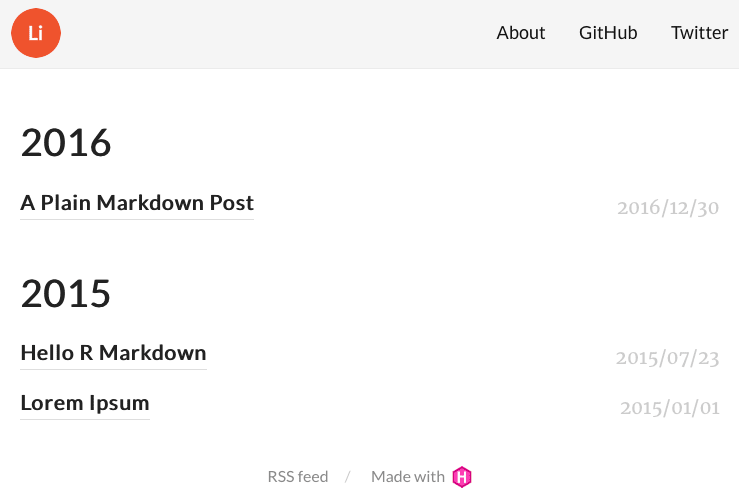
\includegraphics[width=0.9\linewidth]{images/lithium-theme} 

}

\caption{The homepage of the default new site.}\label{fig:lithium}
\end{figure}

You have to know three most basic concepts for a Hugo-based website:

\begin{enumerate}
\def\labelenumi{\arabic{enumi}.}
\item
  The configuration file \texttt{config.toml}\index{config.toml}, in
  which you can specify some global settings for your site. Even if you
  do not know what TOML is at this point (it will be introduced in
  Chapter \ref{hugo}), you may still be able to change some obvious
  settings. For example, you may see configurations like these in
  \texttt{config.toml}:

\begin{Shaded}
\begin{Highlighting}[]
\NormalTok{baseurl }\OperatorTok{=} \StringTok{"/"}
\NormalTok{languageCode }\OperatorTok{=} \StringTok{"en-us"}
\NormalTok{title }\OperatorTok{=} \StringTok{"A Hugo website"}
\NormalTok{theme }\OperatorTok{=} \StringTok{"hugo-lithium-theme"}

\NormalTok{[[}\VariableTok{menu}\NormalTok{.}\AttributeTok{main}\NormalTok{]]}
\NormalTok{    name }\OperatorTok{=} \StringTok{"About"}
\NormalTok{    url }\OperatorTok{=} \StringTok{"/about/"}
\NormalTok{[[}\VariableTok{menu}\NormalTok{.}\AttributeTok{main}\NormalTok{]]}
\NormalTok{    name }\OperatorTok{=} \StringTok{"GitHub"}
\NormalTok{    url }\OperatorTok{=} \StringTok{"https://github.com/rstudio/blogdown"}
\NormalTok{[[}\VariableTok{menu}\NormalTok{.}\AttributeTok{main}\NormalTok{]]}
\NormalTok{    name }\OperatorTok{=} \StringTok{"Twitter"}
\NormalTok{    url }\OperatorTok{=} \StringTok{"https://twitter.com/rstudio"}
\end{Highlighting}
\end{Shaded}

  You can change the website title, e.g.,
  \texttt{title\ =\ "My\ own\ cool\ website"}, and update the GitHub and
  Twitter URLs.\index{Directories}
\item
  The content directory (by default, \texttt{content/}). This is where
  you write the R Markdown or Markdown source files for your posts and
  pages. Under \texttt{content/} of the default site, you can see
  \texttt{about.md} and a \texttt{post/} directory containing a few
  posts. The organization of the content directory is up to you. You can
  have arbitrary files and directories there, depending on the website
  structure you want.
\item
  The publishing directory (by default, \texttt{public/}). Your website
  will be generated to this directory, meaning that you do not need to
  manually add any files to this directory.\footnote{By running either
    \texttt{serve\_site()} or \texttt{build\_site()}, files will be
    generated and published in your publishing directory automatically.}
  Typically it contains a lot of \texttt{*.html} files and dependencies
  like \texttt{*.css}, \texttt{*.js}, and images. You can upload
  everything under \texttt{public/} to any web server that can serve
  static websites, and your website will be up and running. There are
  many options for publishing static websites, and we will talk more
  about them in Chapter \ref{deployment} if you are not familiar with
  deploying websites.
\end{enumerate}

If you are satisfied with this default theme, you are basically ready to
start writing and publishing your new website! We will show how to use
other themes in Section \ref{other-themes}. However, please keep in mind
that a more complicated and fancier theme may require you to learn more
about all the underlying technologies like the Hugo templating language,
HTML, CSS, and JavaScript.

\section{RStudio IDE}\label{rstudio-ide}

There are a few essential RStudio addins\index{RStudio addins} to make
it easy to edit and preview your website, and you can find them in the
menu ``Addins'' on the RStudio toolbar:

\begin{itemize}
\item
  ``Serve Site'': This addin calls \texttt{blogdown::serve\_site()} to
  continuously serve your website locally using the LiveReload
  technology, so you can live preview the website. You can continue to
  edit material for your site while you are previewing it, but this
  function will block your R console by default, meaning that you will
  not be able to use your R console once you start this local web
  server. To unblock your console, click on the red stop sign in the top
  right corner of the console window. If you would rather avoid this
  behavior altogether, set the option
  \texttt{options(servr.daemon\ =\ TRUE)} before you click this addin or
  call the function \texttt{serve\_site()}, so that the server is
  daemonized and will not block your R console.\footnote{We have heard
    of cases where the daemonized server crashed R on Windows. If you
    run into problems with the daemonized server, there are three
    workarounds, and you can try one of them: (1) install the
    \textbf{later} package via \texttt{install.packages("later")} and
    start the server again; (2) use Hugo's server (see Section
    \ref{livereload}); (3) call \texttt{blogdown::serve\_site()} in a
    separate R session, and you can preview your website in your web
    browser but can still edit the website in RStudio.}
\item
  ``New Post'': This addin provides a dialog box for you to enter the
  metadata of your blog post, including the title, author, date, and so
  on. See Figure \ref{fig:new-post} for an example. This addin actually
  calls the function \texttt{blogdown::new\_post()} under the hood, but
  does a few things automatically:

  \begin{itemize}
  \item
    As you type the title of the post, it will generate a filename for
    you, and you can edit it if you do not like the automatically
    generated one. In fact, you can also use this addin to create normal
    pages under any directories under \texttt{content/}. For example, if
    you want to add a resume page, you can change the filename to
    \texttt{resume.md} from the default
    \texttt{post/YYYY-mm-dd-resume.md}.
  \item
    You can select the date from a calendar widget provided by
    Shiny.\footnote{Shiny is an R package for building interactive web
      apps using R. Using this addin, the calendar widget allows you to
      view an interactive calendar by month to select dates. This is a
      simple use of Shiny, but you can read more about Shiny apps here:
      \url{https://shiny.rstudio.com}.}
  \item
    It will scan the categories and tags of existing posts, so when you
    want to input categories or tags, you can select them from the
    dropdown menus, or create new ones.
  \item
    After a new post is created, it will be automatically opened, so you
    can start writing the content immediately.
  \end{itemize}
\item
  ``Update Metadata'': This addin allows you to update the YAML metadata
  of the currently opened post. See Figure \ref{fig:update-meta} for an
  example. The main advantage of this addin is that you can select
  categories and tags from dropdown menus instead of having to remember
  them.
\end{itemize}

\begin{figure}

{\centering 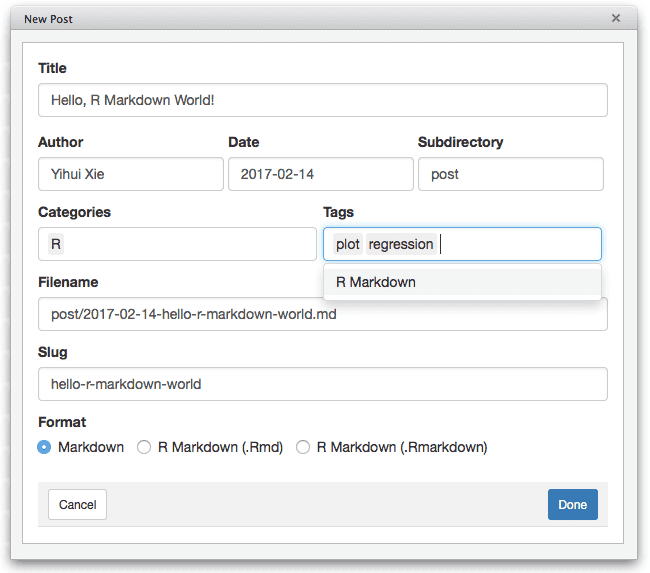
\includegraphics[width=0.8\linewidth]{images/new-post} 

}

\caption{Create a new post using the RStudio addin.}\label{fig:new-post}
\end{figure}

\begin{figure}

{\centering 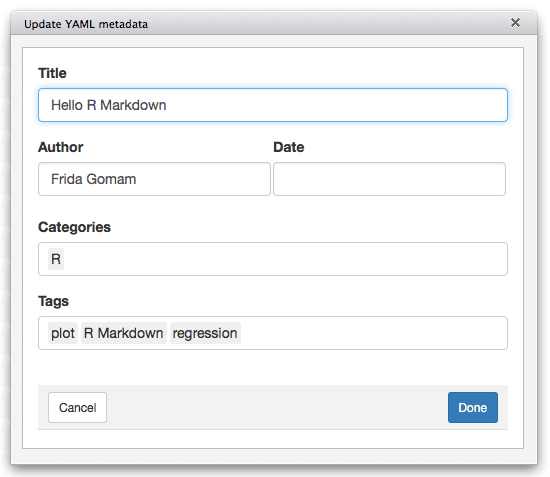
\includegraphics[width=0.7\linewidth]{images/update-meta} 

}

\caption{Update the metadata of an existing post using the RStudio addin.}\label{fig:update-meta}
\end{figure}

With these addins, you should rarely need to run any R commands manually
after you have set up your website, since all your posts will be
automatically compiled whenever you create a new post or modify an
existing post due to the LiveReload feature.

If your RStudio version is at least v1.1.383,\footnote{You may download
  all RStudio official releases including v1.1.383 from
  \url{https://www.rstudio.com/products/rstudio/download/}.} you can
actually create a website project directly from the menu
\texttt{File\ -\textgreater{}\ New\ Project\ -\textgreater{}\ New\ Directory}
(see Figure \ref{fig:new-project} and \ref{fig:blogdown-project}).

\begin{figure}

{\centering 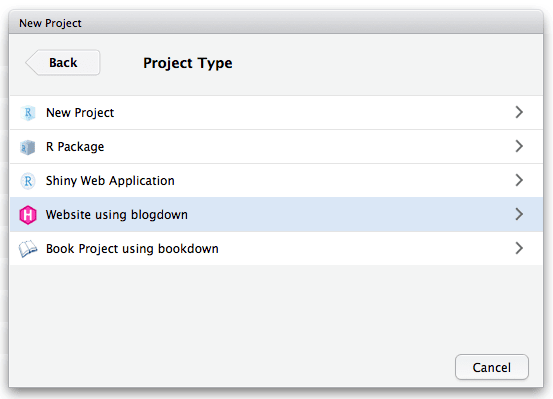
\includegraphics[width=0.8\linewidth]{images/new-project} 

}

\caption{Create a new website project in RStudio.}\label{fig:new-project}
\end{figure}

\begin{figure}

{\centering 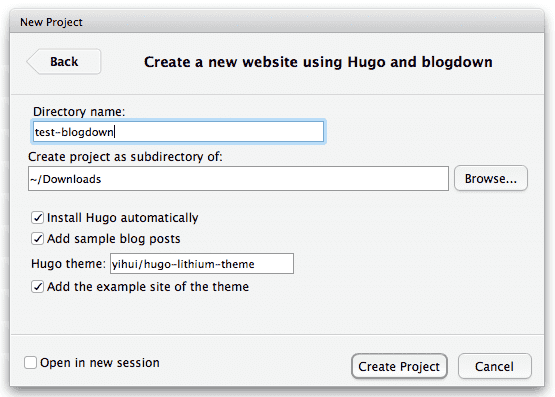
\includegraphics[width=0.8\linewidth]{images/blogdown-project} 

}

\caption{Create a website project based on blogdown.}\label{fig:blogdown-project}
\end{figure}

If your website was created using the function
\texttt{blogdown::new\_site()} instead of the RStudio menu for the first
time, you can quit RStudio and open the project again. If you go to the
menu \texttt{Tools\ -\textgreater{}\ Project\ Options}, your project
type should be ``Website'' like what you can see in Figure
\ref{fig:project-options}.

Then you will see a pane in RStudio named ``Build,'' and there is a
button ``Build Website.'' When you click this button, RStudio will call
\texttt{blogdown::build\_site()} to build the website. This will
automatically generate files in the \texttt{public/}
directory.\footnote{Or wherever your publishing directory is located. It
  is \texttt{public/} by default, but it can be changed by specifying
  the \texttt{publishDir\ =\ "myNewDirectory"} in the
  \texttt{config.toml} file.} If you want to build the website and
publish the output files under the \texttt{public/} manually, you are
recommended to restart your R session and click this ``Build Website''
button every time before you publish the website, instead of publishing
the \texttt{public/} folder generated continuously and automatically by
\texttt{blogdown::serve\_site()}, because the latter calls
\texttt{blogdown::build\_site(local\ =\ TRUE)}, which has some subtle
differences with \texttt{blogdown::build\_site(local\ =\ FALSE)} (see
Section \ref{local-preview} for details).

We strongly recommend that you uncheck the option ``Preview site after
building'' in your RStudio project options (Figure
\ref{fig:project-options}).\footnote{In case you wonder why: unless you
  have set the option \texttt{relativeurls} to \texttt{true} in
  \texttt{config.toml}, it requires a web server to preview the website
  locally, otherwise even if you can see the homepage of your website in
  the RStudio Viewer, most links like those links to CSS and JavaScript
  files are unlikely to work. When the RStudio Viewer shows you the
  preview, it does not actually launch a web server.} You can also
uncheck the option ``Re-knit current preview when supporting files
change,'' since this option is not really useful after you call
\texttt{serve\_site()}.

\begin{figure}

{\centering 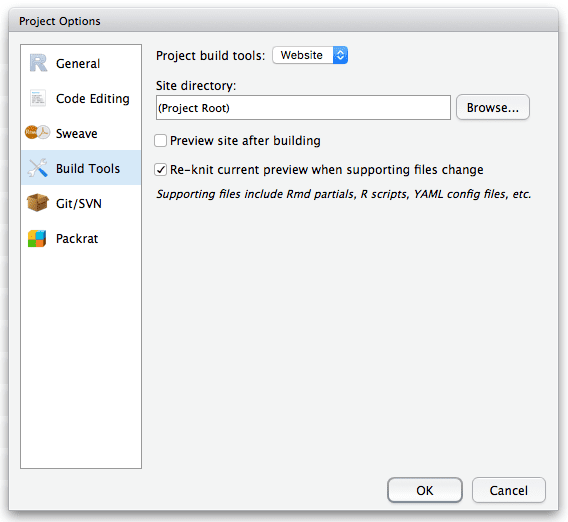
\includegraphics[width=0.8\linewidth]{images/project-options} 

}

\caption{RStudio project options.}\label{fig:project-options}
\end{figure}

\section{\texorpdfstring{Global
options\index{Global Options}}{Global options}}\label{global-options}

Depending on your personal preferences, you can set a few global options
before you work on your website. These options should be set using
\texttt{options(name\ =\ value)}, and currently available options are
presented in Table \ref{tab:global-options}.

\begin{table}

\caption{\label{tab:global-options}Global options that affect the behavior of blogdown.}
\centering
\begin{tabular}[t]{lll}
\toprule
Option name & Default & Meaning\\
\midrule
servr.daemon & FALSE & Whether to use a daemonized server\\
blogdown.author &  & The default author of new posts\\
blogdown.ext & .md & Default extension of new posts\\
blogdown.subdir & post & A subdirectory under content/\\
blogdown.yaml.empty & TRUE & Preserve empty fields in YAML?\\
\bottomrule
\end{tabular}
\end{table}

We recommend that you set these options in your R startup profile file.
You can check out the help page \texttt{?Rprofile} for more details, and
here is a simplified introduction. A startup profile file is basically
an R script that is executed when your R session is started. This is a
perfect place to set global options, so you do not need to type these
options again every time you start a new R session. You can use a global
profile file \texttt{\textasciitilde{}/.Rprofile},\footnote{The tilde
  \texttt{\textasciitilde{}} denotes your home directory in your system.}
or a per-project file \texttt{.Rprofile} under the root directory of
your RStudio project. The former will be applied to all R sessions that
you start, unless you have provided the latter to override it. The
easiest way to create such a file is to use \texttt{file.edit()} in
RStudio, e.g.,

\begin{Shaded}
\begin{Highlighting}[]
\KeywordTok{file.edit}\NormalTok{(}\StringTok{'~/.Rprofile'}\NormalTok{)}
\CommentTok{# or file.edit('.Rprofile')}
\end{Highlighting}
\end{Shaded}

Suppose you always prefer the daemonized server and want the author of
new posts to be ``John Doe'' by default. You can set these options in
the profile file:

\begin{Shaded}
\begin{Highlighting}[]
\KeywordTok{options}\NormalTok{(}\DataTypeTok{servr.daemon =} \OtherTok{TRUE}\NormalTok{, }\DataTypeTok{blogdown.author =} \StringTok{'John Doe'}\NormalTok{)}
\end{Highlighting}
\end{Shaded}

A nice consequence of setting these options is that when you use the
RStudio addin ``New Post,'' the fields ``Author,'' ``Subdirectory,'' and
``Format'' will be automatically populated, so you do not need to
manipulate them every time unless you want to change the defaults
(occasionally).

R only reads one startup profile file. For example, if you have a
\texttt{.Rprofile} under the current directory and a global
\texttt{\textasciitilde{}/.Rprofile}, only the former one will be
executed when R starts up from the current directory. This may make it
inconvenient for multiple authors collaborating on the same website
project, since you cannot set author-specific options. In particular, it
is not possible to set the \texttt{blogdown.author} option in a single
\texttt{.Rprofile}, because this option should be different for
different authors. One workaround is to set common options in
\texttt{.Rprofile} under the root directory of the website project, and
also execute the global \texttt{\textasciitilde{}/.Rprofile} if it
exists. Author-specific options can be set in the global
\texttt{\textasciitilde{}/.Rprofile} on each author's computer.

\begin{Shaded}
\begin{Highlighting}[]
\CommentTok{# in .Rprofile of the website project}
\ControlFlowTok{if}\NormalTok{ (}\KeywordTok{file.exists}\NormalTok{(}\StringTok{'~/.Rprofile'}\NormalTok{)) \{}
\NormalTok{  base}\OperatorTok{::}\KeywordTok{sys.source}\NormalTok{(}\StringTok{'~/.Rprofile'}\NormalTok{, }\DataTypeTok{envir =} \KeywordTok{environment}\NormalTok{())}
\NormalTok{\}}
\CommentTok{# then set options(blogdown.author = 'Your Name') in ~/.Rprofile}
\end{Highlighting}
\end{Shaded}

\section{R Markdown vs.~Markdown}\label{output-format}

If you are not familiar with R Markdown\index{R Markdown}, please see
Appendix \ref{r-markdown} for a quick tutorial. When you create a new
post, you have to decide whether you want to use R Markdown or plain
Markdown\index{Markdown}, as you can see from Figure \ref{fig:new-post}.
The main differences are:

\begin{enumerate}
\def\labelenumi{\arabic{enumi}.}
\item
  You cannot execute any R code in a plain Markdown document, whereas in
  an R Markdown document, you can embed R code chunks
  (\texttt{\textasciigrave{}\textasciigrave{}\textasciigrave{}\{r\}}).
  However, you can still embed R code in plain Markdown using the syntax
  for fenced code blocks
  \texttt{\textasciigrave{}\textasciigrave{}\textasciigrave{}r} (note
  there are no curly braces \texttt{\{\}}). Such code blocks will not be
  executed and may be suitable for pure demonstration purposes. Below is
  an example of an R code chunk in R Markdown:

\begin{Shaded}
\begin{Highlighting}[]
\NormalTok{```\{r cool-plot, fig.width='80%', fig.cap='A cool plot.'\}}
\NormalTok{plot(cars, pch = 20)  # not really cool}
\NormalTok{```}
\end{Highlighting}
\end{Shaded}

  And here is an example of an R code block in plain Markdown:

\begin{Shaded}
\begin{Highlighting}[]
\NormalTok{```r}
\NormalTok{1 + 1  # not executed}
\NormalTok{```}
\end{Highlighting}
\end{Shaded}
\item
  A plain Markdown post is rendered to HTML through
  \href{https://gohugo.io/overview/configuration/}{Blackfriday}
  \index{Blackfriday}(a package written in the Go language and adopted
  by Hugo). An R Markdown document is compiled through the packages
  \textbf{rmarkdown}, \textbf{bookdown}, and Pandoc\index{Pandoc}, which
  means you can use most features of
  \href{http://pandoc.org/MANUAL.html\#pandocs-markdown}{Pandoc's
  Markdown} and
  \href{https://bookdown.org/yihui/bookdown/components.html}{\textbf{bookdown}'s
  Markdown extensions} in \textbf{blogdown}. If you use R Markdown
  \citep{R-rmarkdown} with \textbf{blogdown}, we recommend that you read
  the documentation of Pandoc and \textbf{bookdown} at least once to
  know all the possible features. We will not repeat the details in this
  book, but list the features briefly below, which are also demonstrated
  on the example website \url{https://blogdown-demo.rbind.io}.

  \begin{itemize}
  \item
    Inline formatting: \texttt{\_italic\_} / \texttt{**bold**} text and
    \texttt{\textasciigrave{}inline\ code\textasciigrave{}}.
  \item
    Inline elements: subscripts (e.g.,
    \texttt{H\textasciitilde{}2\textasciitilde{}0}) and superscripts
    (e.g., \texttt{R\^{}2\^{}}); links (\texttt{{[}text{]}(url)}) and
    images \texttt{!{[}title{]}(url)}; footnotes
    \texttt{text\^{}{[}footnote{]}}.
  \item
    Block-level elements: paragraphs; numbered and unnumbered section
    headers; ordered and unordered lists; block quotations; fenced code
    blocks; tables; horizontal rules.
  \item
    Math expressions and equations.
  \item
    Theorems and proofs.
  \item
    R code blocks that can be used to produce text output (including
    tables) and graphics. Note that equations, theorems, tables, and
    figures can be numbered and cross-referenced.
  \item
    Citations and bibliography.
  \item
    HTML widgets, and Shiny apps embedded via
    \texttt{\textless{}iframe\textgreater{}}.
  \end{itemize}
\end{enumerate}

There are many differences in syntax between Blackfriday's Markdown and
Pandoc's Markdown. For example, you can write a task list with
Blackfriday but not with Pandoc:

\begin{Shaded}
\begin{Highlighting}[]
\NormalTok{- }\FloatTok{[x] Write an R package.}
\FloatTok{- [ ] Write a book.}
\FloatTok{- [ ] ...}
\FloatTok{- [ ] Profit!}
\end{Highlighting}
\end{Shaded}

Similarly, Blackfriday does not support LaTeX math and Pandoc does. We
have added the \href{https://www.mathjax.org/\#docs}{MathJax}
\index{MathJax} support to the default theme
(\href{https://github.com/yihui/hugo-lithium-theme}{hugo-lithium-theme})
in \textbf{blogdown} to render LaTeX math on HTML pages, but there is a
caveat for plain Markdown posts: you have to include inline math
expressions in a pair of backticks
\texttt{\textasciigrave{}\$math\$\textasciigrave{}}, e.g.,
\texttt{\textasciigrave{}\$S\_n\ =\ \textbackslash{}sum\_\{i=1\}\^{}n\ X\_i\$\textasciigrave{}}.
Similarly, math expressions of the display style have to be written in
\texttt{\textasciigrave{}\$\$math\$\$\textasciigrave{}}. For R Markdown
posts, you can use \texttt{\$math\$} for inline math expressions, and
\texttt{\$\$math\$\$} for display-style expressions.\footnote{The reason
  that we need the backticks for plain Markdown documents is that we
  have to prevent the LaTeX code from being interpreted as Markdown by
  Blackfriday. Backticks will make sure the inner content is not
  translated as Markdown to HTML, e.g.,
  \texttt{\textasciigrave{}\$\$x\ *y*\ z\$\$\textasciigrave{}} will be
  converted to
  \texttt{\textless{}code\textgreater{}\$\$x\ *y*\ z\$\$\textless{}/code\textgreater{}}.
  Without the backticks, it will be converted to
  \texttt{\$\$x\ \textless{}em\textgreater{}y\textless{}/em\textgreater{}\ z\$\$},
  which is not a valid LaTeX math expression for MathJax. Similar issues
  can arise when you have other special characters like underscores in
  your math expressions.}

If you find it is a pain to have to remember the differences between R
Markdown and Markdown, a conservative choice is to always use R
Markdown, even if your document does not contain any R code chunks.
Pandoc's Markdown is much richer than Blackfriday, and there are only a
small number of features unavailable in Pandoc but present in
Blackfriday. The main disadvantages of using R Markdown are:

\begin{enumerate}
\def\labelenumi{\arabic{enumi}.}
\item
  You may sacrifice some speed in rendering the website, but this may
  not be noticeable due to a caching mechanism in \textbf{blogdown}
  (more on this in Section \ref{local-preview}). Hugo is very fast when
  processing plain Markdown files, and typically it should take less
  than one second to render a few hundred Markdown files.
\item
  You will have some intermediate HTML files in the source directory of
  your website, because \textbf{blogdown} has to call \textbf{rmarkdown}
  to pre-render \texttt{*.Rmd} files \texttt{*.html}. You will also have
  intermediate folders for figures (\texttt{*\_files/}) and cache
  (\texttt{*\_cache/}) if you have plot output in R code chunks or have
  enabled \textbf{knitr}'s caching. Unless you care a lot about the
  ``cleanness'' of the source repository of your website (especially
  when you use a version control tool like GIT), these intermediate
  files should not matter.
\end{enumerate}

In this book, we usually mean \texttt{.Rmd} files when we say ``R
Markdown documents,'' which are compiled to \texttt{.html} by default.
However, there is another type of R Markdown document with the filename
extension \texttt{.Rmarkdown}. Such R Markdown documents are compiled to
Markdown documents with the extension \texttt{.markdown}, which will be
processed by Hugo instead of Pandoc. There are two major limitations of
using \texttt{.Rmarkdown} compared to \texttt{.Rmd}:

\begin{itemize}
\item
  You cannot use Markdown features only supported by Pandoc, such as
  citations. Math expressions only work if you have installed the
  \textbf{xaringan} package \citep{R-xaringan} and applied the
  JavaScript solution mentioned in Section \ref{javascript}.
\item
  HTML widgets are not supported.
\end{itemize}

The main advantage of using \texttt{.Rmarkdown} is that the output files
are cleaner because they are Markdown files. It can be easier for you to
read the output of your posts without looking at the actual web pages
rendered. This can be particularly helpful when reviewing GitHub pull
requests. Note that numbered tables, figures, equations, and theorems
are also supported. You cannot directly use Markdown syntax in table or
figure captions, but you can use text references as a workaround (see
\textbf{bookdown}'s documentation).

For any R Markdown documents (not specific to \textbf{blogdown}), you
have to specify an output format. There are many
\href{http://rmarkdown.rstudio.com/lesson-9.html}{possible output
formats} in the \textbf{rmarkdown} package (such as
\texttt{html\_document} and \texttt{pdf\_document}) and other extension
packages (such as \texttt{tufte::tufte\_html} and
\texttt{bookdown::gitbook}). Of course, the output format for websites
should be HTML. We have provided an output format function
\texttt{blogdown::html\_page} in \textbf{blogdown}, and all R Markdown
files are rendered using this format. It is based on the output format
\texttt{bookdown::html\_document2}, which means it has inherited a lot
of features from \textbf{bookdown} in addition to features in Pandoc.
For example, you can number and cross-reference math equations, figures,
tables, and theorems, etc. See Chapter 2 of the \textbf{bookdown} book
\citep{xie2016} for more details on the syntax.

Note that the output format \texttt{bookdown::html\_document2} in turn
inherits from \texttt{rmarkdown::html\_document}, so you need to see the
help page \texttt{?rmarkdown::html\_document} for all possible options
for the format \texttt{blogdown::html\_page}. If you want to change the
default values of the options of this output format, you can add an
\texttt{output} field to your YAML metadata. For example, we can add a
table of contents to a page, set the figure width to be 6 inches, and
use the \texttt{svg} device for plots by setting these options in YAML:

\begin{Shaded}
\begin{Highlighting}[]
\OtherTok{---}
\FunctionTok{title:}\AttributeTok{ }\StringTok{"My Awesome Post"}
\FunctionTok{author:}\AttributeTok{ }\StringTok{"John Doe"}
\FunctionTok{date:}\AttributeTok{ }\StringTok{"2017-02-14"}
\FunctionTok{output:}
  \FunctionTok{blogdown:}\AttributeTok{:html_page:}
    \FunctionTok{toc:}\AttributeTok{ true}
    \FunctionTok{fig_width:}\AttributeTok{ 6}
    \FunctionTok{dev:}\AttributeTok{ }\StringTok{"svg"}
\OtherTok{---}
\end{Highlighting}
\end{Shaded}

To set options for \texttt{blogdown::html\_page()} globally (i.e., apply
certain options to all Rmd files), you can create a
\texttt{\_output.yml} file under the root directory of your website.
This YAML file should contain the output format directly (do not put the
output format under the \texttt{output} option), e.g.,

\begin{Shaded}
\begin{Highlighting}[]
\FunctionTok{blogdown:}\AttributeTok{:html_page:}
  \FunctionTok{toc:}\AttributeTok{ true}
  \FunctionTok{fig_width:}\AttributeTok{ 6}
  \FunctionTok{dev:}\AttributeTok{ }\StringTok{"svg"}
\end{Highlighting}
\end{Shaded}

At the moment, not all features of \texttt{rmarkdown::html\_document}
are supported in \textbf{blogdown}, such as \texttt{df\_print},
\texttt{code\_folding}, \texttt{code\_download}, and so on.

If your code chunk has graphics output, we recommend that you avoid
special characters like spaces in the chunk label. Ideally, you should
only use alphanumeric characters and dashes, e.g.,
\texttt{\textasciigrave{}\textasciigrave{}\textasciigrave{}\{r,\ my-label\}}
instead of
\texttt{\textasciigrave{}\textasciigrave{}\textasciigrave{}\{r,\ my\ label\}}.

It is not recommended to change the \textbf{knitr} chunk options
\texttt{fig.path} or \texttt{cache.path} in R Markdown. The default
values of these options work best with \textbf{blogdown}. Please read
Section \ref{dep-path} to know the technical reasons if you prefer.

If you are working on an R Markdown post, but do not want
\textbf{blogdown} to compile it, you can temporarily change its filename
extension from \texttt{.Rmd} to another unknown extension such as
\texttt{.Rmkd}.

\section{Other themes}\label{other-themes}

In Hugo, themes\index{Themes} control the entire appearance and
functionality of your site. So, if you care a lot about the appearance
of your website, you will probably spend quite a bit of time in the
beginning looking for a Hugo theme that you like from the collection
listed at \url{http://themes.gohugo.io}. Please note that not all themes
have been tested against \textbf{blogdown}. If you find a certain theme
does not work well with \textbf{blogdown}, you may report to
\url{https://github.com/rstudio/blogdown/issues}, and we will try to
investigate the reason, but it can be time-consuming to learn and
understand how a new theme works, so we recommend that you learn more
about Hugo by yourself before asking, and we also encourage users to
help each other there.

After you have found a satisfactory theme, you need to figure out its
GitHub username and repository name,\footnote{For most themes, you can
  find this by navigating to the theme of your choice from
  \url{http://themes.gohugo.io} and then clicking on \texttt{Homepage}.}
then either install the theme via\index{blogdown::install\_theme()}
\texttt{blogdown::install\_theme()}, or just create a new site under
another new directory and pass the GitHub repository name to the
\texttt{theme} argument of \texttt{new\_site()}. We recommend that you
use the second approach, because Hugo themes could be very complicated
and the usage of each theme can be very different and highly dependent
on \texttt{config.toml}. If you install a theme using
\texttt{install\_theme()} instead of \texttt{new\_site()} you'll need to
manually create the \texttt{config.toml} file in the root directory of
your website to match the newly installed theme.\footnote{In a
  workaround, if you used \texttt{install\_theme()} and set the
  \texttt{theme\_example} argument to TRUE, then you can access an
  example \texttt{config.toml} file. In the \texttt{themes/} directory,
  navigate to the file for your newly downloaded theme and find
  \texttt{exampleSite/config.toml}. This file can be copied to your root
  directory (to replace the \texttt{config.toml} file from your original
  theme) or used as a template to correctly write a new
  \texttt{config.toml} file for your new theme.}

\begin{Shaded}
\begin{Highlighting}[]
\CommentTok{# for example, create a new site with the academic theme}
\NormalTok{blogdown}\OperatorTok{::}\KeywordTok{new_site}\NormalTok{(}\DataTypeTok{theme =} \StringTok{'gcushen/hugo-academic'}\NormalTok{)}
\end{Highlighting}
\end{Shaded}

To save you some time, we list a few themes below that match our taste:

\begin{itemize}
\item
  Simple/minimal themes:
  \href{https://github.com/yihui/hugo-xmin}{XMin,}
  \href{https://github.com/road2stat/hugo-tanka}{Tanka,}
  \href{https://github.com/AlexFinn/simple-a}{simple-a,} and
  \href{https://github.com/jbub/ghostwriter}{ghostwriter.}
\item
  Sophisticated themes:
  \href{https://github.com/gcushen/hugo-academic}{hugo-academic}
  (strongly recommended for users in academia),
  \href{https://github.com/kakawait/hugo-tranquilpeak-theme}{hugo-tranquilpeak-theme,}
  \href{https://github.com/kishaningithub/hugo-creative-portfolio-theme}{hugo-creative-portfolio-theme,}
  and
  \href{https://github.com/devcows/hugo-universal-theme}{hugo-universal-theme.}
\item
  Multimedia content themes: If you are interested in adding multimedia
  content to your site (such as audio files of a podcast), the
  \href{https://github.com/mattstratton/castanet}{castanet} theme
  provides an excellent framework tailored for this application. An
  example of a site using \textbf{blogdown} with the castanet theme is
  the \href{https://www.r-podcast.org}{R-Podcast.}
\end{itemize}

If you do not understand HTML, CSS, or JavaScript, and have no
experience with Hugo themes or templates, it may take you about 10
minutes to get started with your new website, since you have to accept
everything you are given (such as the default theme); if you do have the
knowledge and experience (and desire to highly customize your site), it
may take you several days to get started. Hugo is really powerful. Be
cautious with power.

Another thing to keep in mind is that the more effort you make in a
complicated theme, the more difficult it is to switch to other themes in
the future, because you may have customized a lot of things that are not
straightforward to port to another theme. So please ask yourself
seriously, ``Do I like this fancy theme so much that I will definitely
not change it in the next couple of years?''

\begin{quote}
If you choose to dig a rather deep hole, someday you will have no choice
but keep on digging, even with tears.

\VA{--- Liyun Chen\footnote{Translated from her Chinese Weibo:
  \url{http://weibo.com/1406511850/Dhrb4toHc} (you cannot view this page
  unless you have logged in).}}{}
\end{quote}

\section{A recommended workflow}\label{workflow}

There are a lot of ways to start building a website and deploy it.
Because of the sheer number of technologies that you need to learn to
fully understand how a website works, we'd like to recommend one
workflow to beginners, so that hopefully they do not need to digest the
rest of this book. This is definitely not the most optimal workflow, but
requires you to know the fewest technical details.

To start a new website:

\begin{enumerate}
\def\labelenumi{\arabic{enumi}.}
\item
  Carefully pick a theme at \url{http://themes.gohugo.io}, and find the
  link to its GitHub repository, which is of the form
  \texttt{https://github.com/user/repo}.
\item
  Create a new project in RStudio, and type the code
  \texttt{blogdown::new\_site(theme\ =\ \textquotesingle{}user/repo\textquotesingle{})}
  in the R console, where \texttt{user/repo} is from the link in Step 1.
\item
  Play with the new site for a while and if you do not like it, you can
  repeat the above steps, otherwise edit the options in
  \texttt{config.toml}. If you do not understand certain options, go to
  the documentation of the theme, which is often the README page of the
  GitHub repository. Not all options have to be changed.
\end{enumerate}

To edit a website:

\begin{enumerate}
\def\labelenumi{\arabic{enumi}.}
\item
  Set \texttt{options(servr.daemon\ =\ TRUE)} unless you have already
  set it in \texttt{.Rprofile}. If this option does not work for you
  (e.g., it crashes your R session), see Section \ref{global-options}
  for a workaround.
\item
  Click the RStudio addin ``Serve Site'' to preview the site in RStudio
  Viewer. This only needs to be done once every time you open the
  RStudio project or restart your R session. Do not click the Knit
  button on the RStudio toolbar.
\item
  Use the ``New Post'' addin to create a new post or page, then start
  writing the content.
\item
  Use the ``Update Metadata'' addin to modify the YAML metadata if
  necessary.
\end{enumerate}

To publish a website if you are not familiar with GIT or GitHub:

\begin{enumerate}
\def\labelenumi{\arabic{enumi}.}
\item
  Restart the R session, and run \texttt{blogdown::hugo\_build()}. You
  should get a \texttt{public/} directory under the root directory of
  your project.
\item
  Log into\index{Netlify} \url{https://www.netlify.com} (you can use a
  GitHub account if you have one). If this is the first time you have
  published this website, you can create a new site, otherwise you may
  update the existing site you created last time. You can drag and drop
  the \texttt{public/} folder from your file viewer to the indicated
  area on the Netlify web page, where it says ``Drag a folder with a
  static site here.''
\item
  Wait for a few seconds for Netlify to deploy the files, and it will
  assign a random subdomain of the form
  \texttt{random-word-12345.netlify.com} to you. You can (and should)
  change this random subdomain to a more meaningful one if it is still
  available.
\end{enumerate}

It can be much easier to publish a website if you are familiar with GIT
and GitHub. We recommend that you create a new site on Netlify from your
GitHub repository that contains the source files of your website, so
that you can enjoy the benefits of continuous deployment instead of
manually uploading the \texttt{public/} folder every time. With this
approach, you do not need to run \texttt{blogdown::hugo\_build()}
locally, because the website can be built on Netlify via Hugo. See
Chapter \ref{deployment} for more information.

\chapter{Hugo}\label{hugo}

In this chapter, we will briefly introduce\index{Hugo} Hugo
(\url{https://gohugo.io}), the static site generator on which
\textbf{blogdown} is based. This chapter is not meant to replace the
official Hugo documentation, but provide a guide to those who are just
getting started with Hugo. When in doubt, please consult the official
Hugo documentation.

\section{Static sites and Hugo}\label{static-sites}

A static site\index{Static Site} often consists of HTML files (with
optional external dependencies like images and JavaScript libraries),
and the web server sends exactly the same content to the web browser no
matter who visits the web pages. There is no dynamic computing on the
server when a page is requested. By comparison, a dynamic site relies on
a server-side language to do certain computing and sends potentially
different content depending on different conditions. A common language
is PHP, and a typical example of a dynamic site is a web forum. For
example, each user has a profile page, but typically this does not mean
the server has stored a different HTML profile page for every single
user. Instead, the server will fetch the user data from a database, and
render the profile page dynamically.

For a static site, each URL you visit often has a corresponding HTML
file stored on the server, so there is no need to compute anything
before serving the file to visitors. This means static sites tend to be
faster in response time than dynamic sites, and they are also much
easier to deploy, since deployment simply means copying static files to
a server. A dynamic site often relies on databases, and you will have to
install more software packages to serve a dynamic site. For more
advantages of static sites, please read the
\href{https://gohugo.io/overview/introduction/}{introduction} on Hugo's
website.

There are many existing static site generators, including Hugo,
\href{http://jekyllrb.com}{Jekyll,} and \href{https://hexo.io}{Hexo,}
etc. Most of them can build general-purpose websites but are often used
to build blogs.

We love Hugo for many reasons, but there are a few that stand out.
Unlike other static site generators, the installation of Hugo is very
simple because it provides a single executable without dependencies for
most operating systems (see Section \ref{installation}). It was also
designed to render hundreds of pages of content faster than comparable
static site generators and can reportedly render a single page in
approximately 1 millisecond. Lastly, the community of Hugo users is very
active both on the \href{https://discuss.gohugo.io}{Hugo discussion
forum} and on \href{https://github.com/gohugoio/hugo/issues}{GitHub
issues.}

Although we think Hugo is a fantastic static site generator, there is
really one and only one major missing feature: the support for R
Markdown. That is basically the whole point of the \textbf{blogdown}
package.\footnote{Another motivation was an easier way to create new
  pages or posts. Static site generators often provide commands to
  create new posts, but you often have to open and modify the new file
  created by hand after using these commands. I was very frustrated by
  this, because I was looking for a graphical user interface where I can
  just fill out the title, author, date, and other information about a
  page, then I can start writing the content right away. That is why I
  provided the RStudio addin ``New Post'' and the function
  \texttt{blogdown::new\_post()}. In the past few years, I hated it
  every time I was about to create a new post either by hand or via the
  Jekyll command line. Finally, I felt addicted to blogging again after
  I finished the RStudio addin.} This missing feature means that you
cannot easily generate results using R code on your web pages, since you
can only use static Markdown documents. Besides, Hugo's default Markdown
engine is ``Blackfriday'', which is less powerful than Pandoc.\footnote{The
  Pandoc support has been added in a Hugo pull request:
  \url{https://github.com/gohugoio/hugo/pull/4060}. However, I think the
  support is quite limited, and I'd recommend that you use the R
  Markdown format instead, because with the official Pandoc support in
  Hugo, you cannot customize the Pandoc command-line options, rendering
  is not cached (it could be slow), and you will not be able to use any
  Markdown extensions from the \textbf{bookdown} package (such as
  numbering figure captions).}

Hugo uses a special file and folder structure to create your website
(Figure \ref{fig:folders}). The rest of this chapter will give more
details on the following files and folders:

\begin{itemize}
\tightlist
\item
  \texttt{config.toml}
\item
  \texttt{content/}
\item
  \texttt{static/}
\item
  \texttt{themes/}
\item
  \texttt{layouts/}
\end{itemize}




\begin{figure}

{\centering 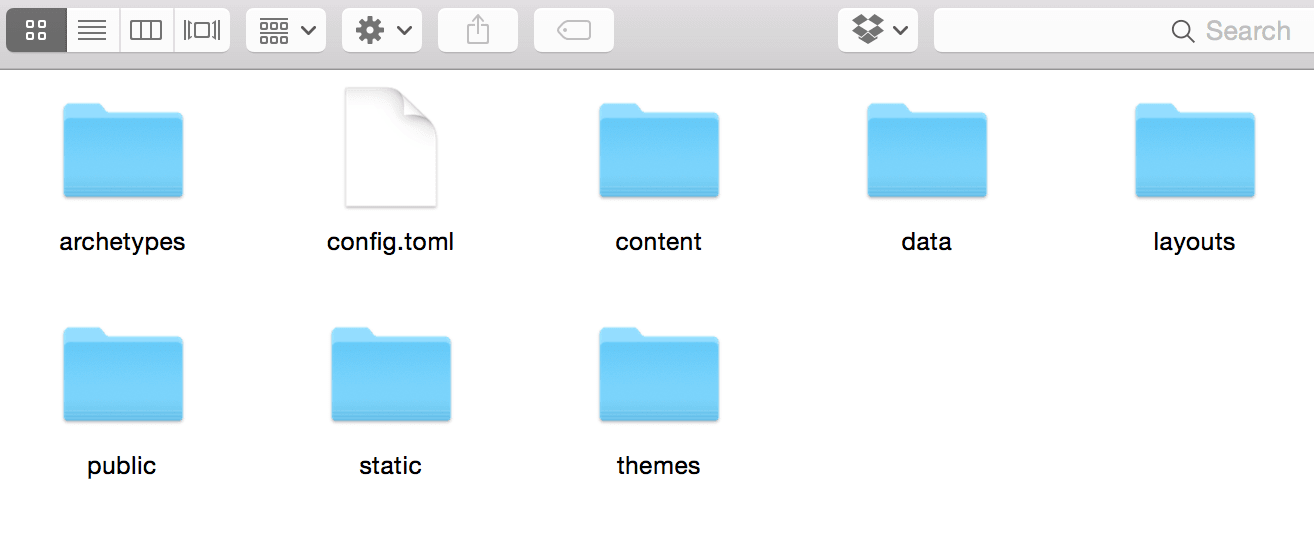
\includegraphics[width=1\linewidth]{images/folder-structure} 

}

\caption{Possible files and folders created when you create a new
site using \textbf{blogdown}.}\label{fig:folders}
\end{figure}

\section{Configuration}\label{configuration}

The first file that you may want to look at is the
configuration\index{config.toml} or \texttt{config} file in your root
directory, in which you can set global configurations of your site. It
may contain options like the title and description of your site, as well
as other global options like links to your social networks, the
navigation menu, and the base URL for your website.

When generating your site, Hugo will search for a file called
\texttt{config.toml} first. If it cannot find one, it will continue to
search for \texttt{config.yaml}.\footnote{Hugo also supports
  \texttt{config.json}, but \textbf{blogdown} does not support it, so we
  do not recommend that you use it.} Since most Hugo themes contain
example sites that ship \texttt{config.toml} files, and the
TOML\index{TOML} (Tom's Obvious, Minimal Language) format appears to be
more popular in the Hugo community, we will mainly discuss
\texttt{config.toml} here.

We recommend that you use the TOML syntax only for the config file (you
can also use YAML if you prefer), and use YAML as the data format for
the metadata of (R) Markdown pages and posts, because R Markdown and
\textbf{blogdown} fully support only YAML\index{YAML}.\footnote{TOML has
  its advantages, but I feel they are not significant in the context of
  Hugo websites. It is a pain to have to know yet another language,
  TOML, when YAML stands for ``Yet Another Markup Language.'' I'm not
  sure if the XKCD comic applies in this case:
  \url{https://xkcd.com/927/}.} If you have a website that has already
used TOML, you may use \texttt{blogdown::hugo\_convert(unsafe\ =\ TRUE)}
to convert TOML data to YAML, but please first make sure you have backed
up the website because it will overwrite your Markdown files.

The Hugo documentation does not use TOML or YAML consistently in its
examples, which can be confusing. Please pay close attention to the
configuration format when copying examples to your own website.

\subsection{TOML Syntax}\label{toml-syntax}

If you are not familiar with the TOML Syntax, we will give a brief
overview and you may read the
\href{https://github.com/toml-lang/toml}{full documentation} to know the
details.

TOML is made up of key-value pairs separated by equal signs:

\begin{Shaded}
\begin{Highlighting}[]
\NormalTok{key }\OperatorTok{=}\NormalTok{ value}
\end{Highlighting}
\end{Shaded}

When you want to edit a configuration in the TOML file, simply change
the value. Values that are character strings should be in quotes,
whereas Boolean values should be lowercase and bare.

For example, if you want to give your website the title ``My Awesome
Site,'' and use relative URLs instead of the default absolute URLs, you
may have the following entries in your \texttt{config.toml} file.

\begin{Shaded}
\begin{Highlighting}[]
\NormalTok{title }\OperatorTok{=} \StringTok{"My Awesome Site"}

\NormalTok{relativeURLs }\OperatorTok{=} \KeywordTok{true}
\end{Highlighting}
\end{Shaded}

Most of your website's global variables are entered in the
\texttt{config.toml} file in exactly this manner.

Further into your \texttt{config} file, you may notice some values in
brackets like this:

\begin{Shaded}
\begin{Highlighting}[]
\NormalTok{[social]}
\NormalTok{    github  }\OperatorTok{=} \StringTok{"https://github.com/rstudio/blogdown"}
\NormalTok{    twitter }\OperatorTok{=} \StringTok{"https://twitter.com/rstudio"}
\end{Highlighting}
\end{Shaded}

This is a table in the TOML language and Hugo uses them to fill in
information on other pages within your site. For instance, the above
table will populate the \texttt{.Site.Social} variable in your site's
templates (more information on this in Section \ref{templates}).

Lastly, you may find some values in double brackets like this:

\begin{Shaded}
\begin{Highlighting}[]
\NormalTok{[[}\VariableTok{menu}\NormalTok{.}\AttributeTok{main}\NormalTok{]]}
\NormalTok{    name }\OperatorTok{=} \StringTok{"Blog"}
\NormalTok{    url }\OperatorTok{=} \StringTok{"/blog/"}

\NormalTok{[[}\VariableTok{menu}\NormalTok{.}\AttributeTok{main}\NormalTok{]]}
\NormalTok{    name }\OperatorTok{=} \StringTok{"Categories"}
\NormalTok{    url }\OperatorTok{=} \StringTok{"/categories/"}

\NormalTok{[[}\VariableTok{menu}\NormalTok{.}\AttributeTok{main}\NormalTok{]]}
\NormalTok{    name }\OperatorTok{=} \StringTok{"About"}
\NormalTok{    url }\OperatorTok{=} \StringTok{"/about/"}
\end{Highlighting}
\end{Shaded}

In TOML, double brackets are used to indicate an array of tables. Hugo
interprets this information as a menu. If the code above was found in a
\texttt{config.toml} file, the resulting website would have links to
Blog, Categories, and About pages in the site's main menu. The location
and styling of that menu are specified elsewhere, but the names of each
menu's choices and the links to each section are defined here.

The \texttt{config.toml} file is different for each theme. Make sure
that when you choose a theme, you read its documentation thoroughly to
get an understanding of what each of the configuration options does
(more on themes in Section \ref{themes}).

\subsection{Options}\label{options}

All built-in options\index{options} that you may set for Hugo are listed
at \url{https://gohugo.io/overview/configuration/}. You can change any
of these options except \texttt{contentDir}, which is hard-coded to
\texttt{content} in \textbf{blogdown}. Our general recommendation is
that you'd better not modify the defaults unless you understand the
consequences. We list a few options that may be of interest to you:

\begin{itemize}
\item
  \texttt{baseURL}: Normally you have to change the value of this option
  to the base URL\index{baseURL} of your website. Some Hugo themes may
  have it set to \texttt{http://replace-this-with-your-hugo-site.com/}
  or \texttt{http://www.example.com/} in their example sites, but please
  make sure to replace them with your own URL (see Chapter
  \ref{deployment} and Appendix \ref{domain-name} for more information
  on publishing websites and obtaining domain names). Note that this
  option can be a URL with a subpath, if your website is to be published
  under a subpath of a domain name, e.g.,
  \texttt{http://www.example.com/docs/}.
\item
  \texttt{enableEmoji}: You\index{Emoji} may set it to \texttt{true} so
  that you can use \href{http://www.emoji-cheat-sheet.com}{Emoji
  emoticons} like \texttt{:smile:} in Markdown.
\item
  \texttt{permalinks}: Rules to generate permanent
  links\index{permalinks} of your pages. By default, Hugo uses full
  filenames under \texttt{content/} to generate links, e.g.,
  \texttt{content/about.md} will be rendered to
  \texttt{public/about/index.html}, and
  \texttt{content/post/2015-07-23-foo.md} will be rendered to
  \texttt{public/post/2015-07-23-foo/index.html}, so the actual links
  are \texttt{/about/} and \texttt{/post/2015-07-23-foo/} on the
  website. Although it is not required to set custom rules for permanent
  links, it is common to see links of the form
  \texttt{/YYYY/mm/dd/post-title/}. Hugo allows you to use several
  pieces of information about a source file to generate a link, such as
  the date (year, month, and day), title, and filename, etc. The link
  can be independent of the actual filename. For example, you may ask
  Hugo to render pages under \texttt{content/post/} using the date and
  title for their links:

\begin{Shaded}
\begin{Highlighting}[]
\NormalTok{[permalinks]}
\NormalTok{    post }\OperatorTok{=} \StringTok{"/:year/:month/:day/:title/"}
\end{Highlighting}
\end{Shaded}

  Personally, I recommend that you use the\index{Slug} \texttt{:slug}
  variable\footnote{A slug is simply a character string that you can use
    to identify a specific post. A slug will not change, even if the
    title changes. For instance, if you decide to change the title of
    your post from ``I love blogdown'' to ``Why blogdown is the best
    package ever,'' and you used the post's title in the URL, your old
    links will now be broken. If instead, you specified the URL via a
    slug (something like ``blogdown-love''), then you can change the
    title as many times as you'd like and you will not end up with any
    broken links.} instead of \texttt{:title}:

\begin{Shaded}
\begin{Highlighting}[]
\NormalTok{[permalinks]}
\NormalTok{    post }\OperatorTok{=} \StringTok{"/:year/:month/:day/:slug/"}
\end{Highlighting}
\end{Shaded}

  This is because your post title may change, and you probably do not
  want the link to the post to change, otherwise you have to redirect
  the old link to the new link, and there will other types of trouble
  like Disqus comments. The \texttt{:slug} variable falls back to
  \texttt{:title} if a field named \texttt{slug} is not set in the YAML
  metadata of the post. You can set a fixed slug so that the link to the
  post is always fixed and you will have the freedom to update the title
  of your post.

  You may find a list of all possible variables that you can use in the
  \texttt{permalinks} option at
  \url{https://gohugo.io/extras/permalinks/}.
\item
  \texttt{publishDir}: The directory under which you want to generate
  the website.
\item
  \texttt{theme}: The directory name of the Hugo theme under
  \texttt{themes/}.
\item
  \texttt{ignoreFiles}: A list of filename patterns (regular
  expressions) for Hugo to ignore\index{ignoreFiles} certain files when
  building the site. I recommend that you specify at least these
  patterns
  \texttt{{[}"\textbackslash{}\textbackslash{}.Rmd\$",\ "\textbackslash{}\textbackslash{}.Rmarkdown\$",\ "\_files\$",\ "\_cache\$"{]}}.
  You should ignore \texttt{.Rmd} files because \textbf{blogdown} will
  compile them to \texttt{.html}, and it suffices for Hugo to use the
  \texttt{.html} files. There is no need for Hugo to build \texttt{.Rmd}
  files, and actually Hugo does not know how. Directories with suffixes
  \texttt{\_files} and \texttt{\_cache} should be ignored because they
  contain auxiliary files after an Rmd file is compiled, and
  \textbf{blogdown} will store them. Hugo should not copy them again to
  the \texttt{public/} directory.
\item
  \texttt{uglyURLs}: By default, Hugo generates ``clean''
  URLs\index{uglyURLs}. This may be a little surprising and requires
  that you understand how URLs work when your browser fetches a page
  from a server. Basically, Hugo generates \texttt{foo/index.html} for
  \texttt{foo.md} by default instead of \texttt{foo.html}, because the
  former allows you to visit the page via the clean URL \texttt{foo/}
  without \texttt{index.html}. Most web servers understand requests like
  \texttt{http://www.example.com/foo/} and will present
  \texttt{index.html} under \texttt{foo/} to you. If you prefer the
  strict mapping from \texttt{*.md} to \texttt{*.html}, you may enable
  ``ugly'' URLs by setting \texttt{uglyURLs} to \texttt{true}.
\item
  \texttt{hasCJKLanguage}: If your website is primarily in
  CJK\index{hasCJKLanguage} (Chinese, Korean, and Japanese), I recommend
  that you set this option to \texttt{true}, so that Hugo's automatic
  summary and word count work better.
\end{itemize}

Besides the built-in Hugo options, you can set other arbitrary options
in \texttt{config.toml}. For example, it is very common to see an option
named \texttt{params}, which is widely used in many Hugo themes. When
you see a variable \texttt{.Site.Params.FOO} in a Hugo theme, it means
an option \texttt{FOO} that you set under \texttt{{[}params{]}} in
\texttt{config.toml}, e.g., \texttt{.Site.Params.author} is
\texttt{Frida\ Gomam} with the following config file:

\begin{Shaded}
\begin{Highlighting}[]
\NormalTok{[params]}
\NormalTok{    author }\OperatorTok{=} \StringTok{"Frida Gomam"}
\NormalTok{    dateFormat }\OperatorTok{=} \StringTok{"2006/01/02"}
\end{Highlighting}
\end{Shaded}

The goal of all these options is to avoid hard-coding anything in Hugo
themes, so that users can easily edit a single config file to apply the
theme to their websites, instead of going through many HTML files and
making changes one by one.

\section{Content}\label{content}

The structure of the \texttt{content/} directory can be arbitrary. A
common structure is that there are a few static pages under the root of
\texttt{content/}, and a subdirectory \texttt{post/} containing blog
posts:

\begin{Shaded}
\begin{Highlighting}[]
\NormalTok{├── }\ExtensionTok{_index.md}
\NormalTok{├── }\ExtensionTok{about.md}
\NormalTok{├── }\ExtensionTok{vitae.md}
\NormalTok{├── }\ExtensionTok{post/}
\NormalTok{│   ├── }\ExtensionTok{2017-01-01-foo.md}
\NormalTok{│   ├── }\ExtensionTok{2017-01-02-bar.md}
\NormalTok{│   └── }\ExtensionTok{...}
\NormalTok{└── }\ExtensionTok{...}
\end{Highlighting}
\end{Shaded}

\subsection{YAML metadata}\label{yaml-metadata}

Each page should start with YAML\index{YAML} metadata specifying
information like the title, date, author, categories, tags, and so on.
Depending on the specific Hugo theme and templates you use, some of
these fields may be optional.

Among all YAML fields, we want to bring these to your attention:

\begin{itemize}
\item
  \texttt{draft}: You can mark a document as a draft\index{Draft} by
  setting \texttt{draft:\ true} in its YAML metadata. Draft posts will
  not be rendered if the site is built via
  \texttt{blogdown::build\_site()} or \texttt{blogdown::hugo\_build()},
  but will be rendered in the local preview mode (see Section
  \ref{local-preview}).
\item
  \texttt{publishdate}: You may specify a future
  date\index{Publish Date} to publish a post. Similar to draft posts,
  future posts are only rendered in the local preview mode.
\item
  \texttt{weight}: This field can take a numeric value to tell Hugo the
  order of pages when sorting them\index{Post Weight}, e.g., when you
  generate a list of all pages under a directory, and two posts have the
  same date, you may assign different weights to them to get your
  desired order on the list.
\item
  \texttt{slug}: A character string as the tail of the URL. It is
  particularly useful when you define custom rules for permanent URLs
  (see Section \ref{options}).
\end{itemize}

\subsection{Body}\label{body}

As we mentioned in Section \ref{output-format}, your post can be written
in either R Markdown or plain Markdown. Please be cautious about the
syntax differences between the two formats when you write the body of a
post.

\subsection{Shortcode}\label{shortcode}

Besides all Markdown features, Hugo provides a useful feature named
``shortcodes.'' You can use a shortcode\index{Shortcode} in the body of
your post. When Hugo renders the post, it can automatically generate an
HTML snippet based on the parameters you pass to the shortcode. This is
convenient because you do not have to type or embed a large amount of
HTML code in your post. For example, Hugo has a built-in shortcode for
embedding Twitter cards. Normally, this is how you embed a Twitter card
(Figure \ref{fig:jtleek-tweet}) on a page:

\begin{Shaded}
\begin{Highlighting}[]
\KeywordTok{<blockquote}\OtherTok{ class=}\StringTok{"twitter-tweet"}\KeywordTok{>}
  \KeywordTok{<p}\OtherTok{ lang=}\StringTok{"en"}\OtherTok{ dir=}\StringTok{"ltr"}\KeywordTok{>}\NormalTok{Anyone know of an R package for}
\NormalTok{    interfacing with Alexa Skills?}
    \KeywordTok{<a}\OtherTok{ href=}\StringTok{"https://twitter.com/thosjleeper"}\KeywordTok{>}\NormalTok{@thosjleeper}\KeywordTok{</a>}
    \KeywordTok{<a}\OtherTok{ href=}\StringTok{"https://twitter.com/xieyihui"}\KeywordTok{>}\NormalTok{@xieyihui}\KeywordTok{</a>}
    \KeywordTok{<a}\OtherTok{ href=}\StringTok{"https://twitter.com/drob"}\KeywordTok{>}\NormalTok{@drob}\KeywordTok{</a>}
    \KeywordTok{<a}\OtherTok{ href=}\StringTok{"https://twitter.com/JennyBryan"}\KeywordTok{>}\NormalTok{@JennyBryan}\KeywordTok{</a>}
    \KeywordTok{<a}\OtherTok{ href=}\StringTok{"https://twitter.com/HoloMarkeD"}\KeywordTok{>}\NormalTok{@HoloMarkeD}\KeywordTok{</a>}\NormalTok{ ?}
  \KeywordTok{</p>}
  \DecValTok{&mdash;}\NormalTok{ Jeff Leek (@jtleek)}
  \KeywordTok{<a}\OtherTok{ href=}\StringTok{"https://twitter.com/jtleek/status/852205086956818432"}\KeywordTok{>}
\NormalTok{    April 12, 2017}
  \KeywordTok{</a>}
\KeywordTok{</blockquote>}
\KeywordTok{<script}\OtherTok{ async src=}\StringTok{"//platform.twitter.com/widgets.js"}\OtherTok{ charset=}\StringTok{"utf-8"}\KeywordTok{>}
\KeywordTok{</script>}
\end{Highlighting}
\end{Shaded}

\begin{figure}

{\centering 
\includegraphics[width=0.8\linewidth]{images/jtleek-tweet} 

}

\caption{A tweet by Jeff Leek.}\label{fig:jtleek-tweet}
\end{figure}

If you use the shortcode, all you need in the Markdown source document
is:

\begin{Shaded}
\begin{Highlighting}[]
\NormalTok{\{\{< tweet }\DecValTok{852205086956818432}\NormalTok{ >\}\}}
\end{Highlighting}
\end{Shaded}

Basically, you only need to pass the ID of the tweet to a shortcode
named \texttt{tweet}. Hugo will fetch the tweet automatically and render
the HTML snippet for you. For more about shortcodes, see
\url{https://gohugo.io/extras/shortcodes/}.

Shortcodes are supposed to work in plain Markdown documents only. To use
shortcodes in R Markdown instead of plain Markdown, you have to call the
function \texttt{blogdown::shortcode()}, e.g.,

\begin{Shaded}
\begin{Highlighting}[]
\NormalTok{```\{r echo=FALSE\}}
\NormalTok{blogdown::shortcode('tweet', '852205086956818432')}
\NormalTok{```}
\end{Highlighting}
\end{Shaded}

\section{Themes}\label{themes}

A Hugo theme\index{Themes} is a collection of template files and
optional website assets such as CSS and JavaScript files. In a nutshell,
a theme defines what your website looks like after your source content
is rendered through the templates.

Hugo has provided a large number of user-contributed themes at
\url{https://themes.gohugo.io}. Unless you are an experienced web
designer, you'd better start from an existing theme here. The quality
and complexity of these themes vary a lot, and you should choose one
with caution. For example, you may take a look at the number of stars of
a theme repository on GitHub, as well as whether the repository is still
relatively active. We do not recommend that you use a theme that has not
been updated for more than a year.

In this section, we will explain how the default theme in
\textbf{blogdown} works, which may also give you some ideas about how to
get started with other themes.

\subsection{The default theme}\label{the-default-theme}

The default theme in \textbf{blogdown},
hugo-lithium-theme\index{Hugo Lithium Theme}, is hosted on GitHub at
\url{https://github.com/yihui/hugo-lithium-theme}. It was originally
written by Jonathan Rutheiser, and I have made several changes to it.
This theme is suitable for those who prefer minimal styles, and want to
build a website with a few pages and some blog posts.

Typically a theme repository on GitHub has a \texttt{README} file, which
also serves as the documentation of the theme. After you read it, the
next file to look for is \texttt{config.toml} under the
\texttt{exampleSite} directory, which contains sample configurations for
a website based on this theme. If a theme does not have a
\texttt{README} file or \texttt{exampleSite} directory, you probably
should not use it.

The \texttt{config.toml} of the theme hugo-lithium-theme contains the
following options:

\begin{Shaded}
\begin{Highlighting}[]
\NormalTok{baseurl }\OperatorTok{=} \StringTok{"/"}
\NormalTok{relativeurls }\OperatorTok{=} \KeywordTok{false}
\NormalTok{languageCode }\OperatorTok{=} \StringTok{"en-us"}
\NormalTok{title }\OperatorTok{=} \StringTok{"A Hugo website"}
\NormalTok{theme }\OperatorTok{=} \StringTok{"hugo-lithium-theme"}
\NormalTok{googleAnalytics }\OperatorTok{=} \StringTok{""}
\NormalTok{disqusShortname }\OperatorTok{=} \StringTok{""}
\NormalTok{ignoreFiles }\OperatorTok{=}\NormalTok{ [}\StringTok{"}\SpecialCharTok{\textbackslash{}\textbackslash{}}\StringTok{.Rmd$"}\OperatorTok{,} \StringTok{"}\SpecialCharTok{\textbackslash{}\textbackslash{}}\StringTok{.Rmarkdown"}\OperatorTok{,} \StringTok{"_files$"}\OperatorTok{,} \StringTok{"_cache$"}\NormalTok{]}

\NormalTok{[permalinks]}
\NormalTok{    post }\OperatorTok{=} \StringTok{"/:year/:month/:day/:slug/"}

\NormalTok{[[}\VariableTok{menu}\NormalTok{.}\AttributeTok{main}\NormalTok{]]}
\NormalTok{    name }\OperatorTok{=} \StringTok{"About"}
\NormalTok{    url }\OperatorTok{=} \StringTok{"/about/"}
\NormalTok{[[}\VariableTok{menu}\NormalTok{.}\AttributeTok{main}\NormalTok{]]}
\NormalTok{    name }\OperatorTok{=} \StringTok{"GitHub"}
\NormalTok{    url }\OperatorTok{=} \StringTok{"https://github.com/rstudio/blogdown"}
\NormalTok{[[}\VariableTok{menu}\NormalTok{.}\AttributeTok{main}\NormalTok{]]}
\NormalTok{    name }\OperatorTok{=} \StringTok{"Twitter"}
\NormalTok{    url }\OperatorTok{=} \StringTok{"https://twitter.com/rstudio"}

\NormalTok{[params]}
\NormalTok{    description }\OperatorTok{=} \StringTok{"A website built through Hugo and blogdown."}

\NormalTok{    highlightjsVersion }\OperatorTok{=} \StringTok{"9.11.0"}
\NormalTok{    highlightjsCDN }\OperatorTok{=} \StringTok{"//cdn.bootcss.com"}
\NormalTok{    highlightjsLang }\OperatorTok{=}\NormalTok{ [}\StringTok{"r"}\OperatorTok{,} \StringTok{"yaml"}\NormalTok{]}
\NormalTok{    highlightjsTheme }\OperatorTok{=} \StringTok{"github"}

\NormalTok{    MathJaxCDN }\OperatorTok{=} \StringTok{"//cdn.bootcss.com"}
\NormalTok{    MathJaxVersion }\OperatorTok{=} \StringTok{"2.7.1"}

\NormalTok{[}\VariableTok{params}\NormalTok{.}\AttributeTok{logo}\NormalTok{]}
\NormalTok{    url }\OperatorTok{=} \StringTok{"logo.png"}
\NormalTok{    width }\OperatorTok{=} \DecValTok{50}
\NormalTok{    height }\OperatorTok{=} \DecValTok{50}
\NormalTok{    alt }\OperatorTok{=} \StringTok{"Logo"}
\end{Highlighting}
\end{Shaded}

Some of these options may be obvious to understand, and some may need
explanations:

\begin{itemize}
\item
  \texttt{baseurl}: You\index{baseURL} can configure this option later,
  after you have a domain name for your website. Do not forget the
  trailing slash.
\item
  \texttt{relativeurls}: This is optional. You may want to set it to
  \texttt{true} only if you intend to view your website locally through
  your file viewer, e.g., double-click on an HTML file and view it in
  your browser. This option defaults to \texttt{false} in Hugo, and it
  means your website must be viewed through a web server, e.g.,
  \texttt{blogdown::serve\_site()} has provided a local web server, so
  you can preview your website locally when
  \texttt{relativeurls\ =\ false}.
\item
  \texttt{title}: The title of your website. Typically this is displayed
  in a web browser's title bar or on a page tab.
\item
  \texttt{theme}: The directory name of the theme. You need to be very
  careful when changing themes, because one theme can be drastically
  different from another theme in terms of the configurations. It is
  quite possible that a different theme will not work with your current
  \texttt{config.toml}. Again, you have to read the documentation of a
  theme to know what options are supported or required.
\item
  \texttt{googleAnalytics}: The Google Analytics\index{Google Analytics}
  tracking ID (like \texttt{UA-000000-2}). You can sign up at
  \url{https://analytics.google.com} to obtain a tracking ID.
\item
  \texttt{disqusShortname}: The Disqus ID\index{Disqus Comments} that
  you created during the account setup process at
  \url{https://disqus.com}. This is required to enable commenting on
  your site.\footnote{As we mentioned in Section \ref{static-sites},
    \textbf{blogdown} generates static and unchanging content. To add
    something dynamic and always changing (like the ability for your
    fans to leave comments), you must incorporate an outside commenting
    system like Disqus.} Please note that you have to set up a
  functional \texttt{baseurl} and publish your website before Disqus
  comments can work.
\item
  \texttt{ignoreFiles} and \texttt{permalinks}: These options have been
  explained in Section \ref{options}.
\item
  \texttt{menu}: This list of options specifies the text and URL of menu
  items at the top. See Figure \ref{fig:lithium} for a sample page. You
  can change or add more menu items. If you want to order the items, you
  may assign a \texttt{weight} to each item, e.g.,

\begin{Shaded}
\begin{Highlighting}[]
\NormalTok{[[}\VariableTok{menu}\NormalTok{.}\AttributeTok{main}\NormalTok{]]}
\NormalTok{    name }\OperatorTok{=} \StringTok{"Home"}
\NormalTok{    url }\OperatorTok{=} \StringTok{"/"}
\NormalTok{    weight }\OperatorTok{=} \DecValTok{1}
\NormalTok{[[}\VariableTok{menu}\NormalTok{.}\AttributeTok{main}\NormalTok{]]}
\NormalTok{    name }\OperatorTok{=} \StringTok{"About"}
\NormalTok{    url }\OperatorTok{=} \StringTok{"/about/"}
\NormalTok{    weight }\OperatorTok{=} \DecValTok{2}
\NormalTok{[[}\VariableTok{menu}\NormalTok{.}\AttributeTok{main}\NormalTok{]]}
\NormalTok{    name }\OperatorTok{=} \StringTok{"GitHub"}
\NormalTok{    url }\OperatorTok{=} \StringTok{"https://github.com/rstudio/blogdown"}
\NormalTok{    weight }\OperatorTok{=} \DecValTok{3}
\NormalTok{[[}\VariableTok{menu}\NormalTok{.}\AttributeTok{main}\NormalTok{]]}
\NormalTok{    name }\OperatorTok{=} \StringTok{"CV"}
\NormalTok{    url }\OperatorTok{=} \StringTok{"/vitae/"}
\NormalTok{    weight }\OperatorTok{=} \DecValTok{4}
\NormalTok{[[}\VariableTok{menu}\NormalTok{.}\AttributeTok{main}\NormalTok{]]}
\NormalTok{    name }\OperatorTok{=} \StringTok{"Twitter"}
\NormalTok{    url }\OperatorTok{=} \StringTok{"https://twitter.com/rstudio"}
\NormalTok{    weight }\OperatorTok{=} \DecValTok{5}
\end{Highlighting}
\end{Shaded}

  In the above example, I added a menu item \texttt{CV} with the URL
  \texttt{/vitae/}, and there is supposed to be a corresponding source
  file \texttt{vitae.md} under the \texttt{content/} directory to
  generate the page \texttt{/vitae/index.html}, so the link will
  actually function.
\item
  \texttt{params}: Miscellaneous parameters\index{params} for the theme.

  \begin{itemize}
  \item
    \texttt{description}: A brief description of your website. It is not
    visible on web pages (you can only see it from the HTML source), but
    should give search engines a hint about your website.
  \item
    \texttt{highlightjs*}: These options are used to configure the
    JavaScript library\index{Syntax Highlighting}
    \href{https://highlightjs.org}{highlight.js} for syntax highlighting
    of code blocks on the web pages. You can change the version (e.g.,
    \texttt{9.12.0}), the CND host (e.g., using
    \href{https://cdnjs.com}{cdnjs}:
    \texttt{//cdnjs.cloudflare.com/ajax/libs}), add more languages
    (e.g., \texttt{{[}"r",\ "yaml",\ "tex"{]}}), and change the theme
    (e.g., \texttt{atom-one-light}). See
    \url{https://highlightjs.org/static/demo/} for all languages and
    themes that highlight.js supports.
  \item
    \texttt{MathJax*}: The JavaScript library MathJax\index{MathJax} can
    render LaTeX math expressions on web pages. Similar to
    \texttt{highlightjsCDN}, you can specify the CDN host of MathJax,
    e.g., \texttt{//cdnjs.cloudflare.com/ajax/libs}, and you can also
    specify the version of MathJax.
  \item
    \texttt{logo}: A list of options to define the logo\index{Logo} of
    the website. By default, the image \texttt{logo.png} under the
    \texttt{static/} directory is used.
  \end{itemize}
\end{itemize}

If you want to be a theme developer and fully understand all the
technical details about these options, you have to understand Hugo
templates, which we will introduce in Section \ref{templates}.

\section{Templates}\label{templates}

A Hugo theme consists of two major components:
templates\index{Templates}, and web assets. The former is essential, and
tells Hugo how to render a page.\footnote{The most common functionality
  of templates is to render HTML pages, but there can also be special
  templates, for example, for RSS feeds and sitemaps, which are XML
  files.} The latter is optional but also important. It typically
consists of CSS and JavaScript files, as well as other assets like
images and videos. These assets determine the appearance and
functionality of your website, and some may be embedded in the content
of your web pages.

You can learn more about Hugo templates from the official documentation
(\url{https://gohugo.io/templates/overview/}). There are a great many
different types of templates. To make it easier for you to master the
key ideas, I created a very minimal Hugo theme, which covers most
functionalities that an average user may need, but the total number of
lines is only about 150, so we can talk about all the source code of
this theme in the following subsection.

\subsection{A minimal example}\label{a-minimal-example}

\href{https://github.com/yihui/hugo-xmin}{XMin} is a Hugo
theme\index{XMin Theme} I wrote from scratch in about 12 hours. Roughly
half an hour was spent on templates, 3.5 hours were spent on tweaking
the CSS styles, and 8 hours were spent on the documentation
(\url{https://xmin.yihui.name}). I think this may be a representative
case of how much time you would spend on each part when designing a
theme. It is perhaps our nature to spend much more time on cosmetic
stuff like CSS than essential stuff like templates. Meanwhile, coding is
often easier than documentation.

We will show the source code of the XMin theme. Because the theme may be
updated occasionally in the future, you may follow this link to obtain a
fixed version that we will talk about in this section:
\url{https://github.com/yihui/hugo-xmin/tree/4bb305}. Below is a tree
view of all files and directories in the theme:

\begin{Shaded}
\begin{Highlighting}[]
\ExtensionTok{hugo-xmin/}
\NormalTok{├── }\ExtensionTok{LICENSE.md}
\NormalTok{├── }\ExtensionTok{README.md}
\NormalTok{├── }\ExtensionTok{archetypes}
\NormalTok{│   └── }\ExtensionTok{default.md}
\NormalTok{├── }\ExtensionTok{layouts}
\NormalTok{│   ├── }\ExtensionTok{404.html}
\NormalTok{│   ├── }\ExtensionTok{_default}
\NormalTok{│   │   ├── }\ExtensionTok{list.html}
\NormalTok{│   │   ├── }\ExtensionTok{single.html}
\NormalTok{│   │   └── }\ExtensionTok{terms.html}
\NormalTok{│   └── }\ExtensionTok{partials}
\NormalTok{│       ├── }\ExtensionTok{foot_custom.html}
\NormalTok{│       ├── }\ExtensionTok{footer.html}
\NormalTok{│       ├── }\ExtensionTok{head_custom.html}
\NormalTok{│       └── }\ExtensionTok{header.html}
\NormalTok{├── }\ExtensionTok{static}
\NormalTok{│   └── }\ExtensionTok{css}
\NormalTok{│       ├── }\ExtensionTok{fonts.css}
\NormalTok{│       └── }\ExtensionTok{style.css}
\NormalTok{└── }\ExtensionTok{exampleSite}
\NormalTok{    ├── }\ExtensionTok{config.toml}
\NormalTok{    ├── }\ExtensionTok{content}
\NormalTok{    │   ├── }\ExtensionTok{_index.md}
\NormalTok{    │   ├── }\ExtensionTok{about.md}
\NormalTok{    │   ├── }\ExtensionTok{note}
\NormalTok{    │   │   ├── }\ExtensionTok{2017-06-13-a-quick-note.md}
\NormalTok{    │   │   └── }\ExtensionTok{2017-06-14-another-note.md}
\NormalTok{    │   └── }\ExtensionTok{post}
\NormalTok{    │       ├── }\ExtensionTok{2015-07-23-lorem-ipsum.md}
\NormalTok{    │       └── }\ExtensionTok{2016-02-14-hello-markdown.md}
\NormalTok{    ├── }\ExtensionTok{layouts}
\NormalTok{    │   └── }\ExtensionTok{partials}
\NormalTok{    │       └── }\ExtensionTok{foot_custom.html}
\NormalTok{    └── }\ExtensionTok{public}
\NormalTok{        └── }\ExtensionTok{...}
\end{Highlighting}
\end{Shaded}

\texttt{LICENSE.md} and \texttt{README.md} are not required components
of a theme, but you definitely should choose a license for your source
code so that other people can properly use your code, and a
\texttt{README} can be the brief documentation of your software.

The file \texttt{archetypes/default.md} defines the default template
based on which users can create new posts. In this theme,
\texttt{default.md} only provided empty YAML metadata:

\begin{Shaded}
\begin{Highlighting}[]
\OtherTok{---}
\OtherTok{---}
\end{Highlighting}
\end{Shaded}

The most important directories of a theme are \texttt{layouts/} and
\texttt{static/}. HTML templates are stored under \texttt{layouts/}, and
assets are stored under \texttt{static/}.

To understand \texttt{layouts/}, you must know some basics about HTML
(see Section \ref{html}) because the templates under this directory are
mostly HTML documents or fragments. There are many possible types of
subdirectories under \texttt{layouts/}, but we are only going to
introduce two here: \texttt{\_default/} and \texttt{partials/}.

\begin{itemize}
\item
  The \texttt{\_default/} directory\index{\_default/} is where you put
  the default templates for your web pages. In the XMin theme, we have
  three templates: \texttt{single.html}, \texttt{list.html}, and
  \texttt{terms.html}.

  \begin{itemize}
  \item
    \texttt{single.html} is a template\index{single.html} for rendering
    single pages. A single page basically corresponds to a Markdown
    document under \texttt{content/}, and it contains both the (YAML)
    metadata and content. Typically we want to render the page title,
    author, date, and the content. Below is the source code of XMin's
    \texttt{single.html}:

\begin{Shaded}
\begin{Highlighting}[]
\NormalTok{\{\{ partial "header.html" . \}\}}
\KeywordTok{<div}\OtherTok{ class=}\StringTok{"article-meta"}\KeywordTok{>}
\KeywordTok{<h1><span}\OtherTok{ class=}\StringTok{"title"}\KeywordTok{>}\NormalTok{\{\{ .Title \}\}}\KeywordTok{</span></h1>}
\NormalTok{\{\{ with .Params.author \}\}}
\KeywordTok{<h2}\OtherTok{ class=}\StringTok{"author"}\KeywordTok{>}\NormalTok{\{\{ . \}\}}\KeywordTok{</h2>}
\NormalTok{\{\{ end \}\}}
\NormalTok{\{\{ if .Params.date \}\}}
\KeywordTok{<h2}\OtherTok{ class=}\StringTok{"date"}\KeywordTok{>}\NormalTok{\{\{ .Date.Format "2006/01/02" \}\}}\KeywordTok{</h2>}
\NormalTok{\{\{ end \}\}}
\KeywordTok{</div>}

\KeywordTok{<main>}
\NormalTok{\{\{ .Content \}\}}
\KeywordTok{</main>}

\NormalTok{\{\{ partial "footer.html" . \}\}}
\end{Highlighting}
\end{Shaded}

    You see a lot of pairs of double curly braces \texttt{\{\{\}\}}, and
    that is how you program the templates using Hugo's variables and
    functions.

    The template starts with a partial template \texttt{header.html},
    for which you will see the source code soon. For now, you can
    imagine it as all the HTML tags before the body of your page (e.g.,
    \texttt{\textless{}html\textgreater{}\textless{}head\textgreater{}}).
    Partial templates\index{Partials} are mainly for reusing HTML code.
    For example, all HTML pages may share very similar
    \texttt{\textless{}head\textgreater{}\textless{}/head\textgreater{}}
    tags, and you can factor out the common parts into partial
    templates.

    The metadata of a page is included in a
    \texttt{\textless{}div\textgreater{}} element with the class
    \texttt{article-meta}. We recommend that you assign classes to HTML
    elements when designing templates, so that it will be easier to
    apply CSS styles to these elements using class names. In a template,
    you have access to many variables provided by Hugo, e.g., the
    \texttt{.Title} variable stores the value of the page title, and we
    write the title in a \texttt{\textless{}span\textgreater{}} in a
    first-level header \texttt{\textless{}h1\textgreater{}}. Similarly,
    the author and date are written in
    \texttt{\textless{}h2\textgreater{}}, but only if they are provided
    in the YAML metadata. The syntax
    \texttt{\{\{\ with\ FOO\ \}\}\{\{\ .\ \}\}\{\{\ end\ \}\}} is a
    shorthand of
    \texttt{\{\{if\ FOO\ \}\}\{\{\ FOO\ \}\}\{\{\ end\ \}\}}, i.e., it
    saves you the effort of typing the expression \texttt{FOO} twice by
    using \texttt{\{\{\ .\ \}\}}. The method \texttt{.Format} can be
    applied to a date object, and in this theme, we format dates in the
    form \texttt{YYYY/mm/dd} (\texttt{2006/01/02} is the way to specify
    the format in Go).

    Then we show the content of a page, which is stored in the variable
    \texttt{.Content}. The content is wrapped in a semantic HTML tag
    \texttt{\textless{}main\textgreater{}}.

    The template is finished after we include another partial template
    \texttt{footer.html} (source code to be shown shortly).

    To make it easier to understand how a template works, we show a
    minimal example post below:

\begin{Shaded}
\begin{Highlighting}[]
\NormalTok{---}
\NormalTok{title: Hello World}
\NormalTok{author: Frida Gomam}
\NormalTok{date: 2017-06-19}
\NormalTok{---}

\NormalTok{A single paragraph.}
\end{Highlighting}
\end{Shaded}

    Using the template \texttt{single.html}, it will be converted to an
    HTML page with source code that looks more or less like this (with
    the header and footer omitted):

\begin{Shaded}
\begin{Highlighting}[]
\KeywordTok{<div}\OtherTok{ class=}\StringTok{"article-meta"}\KeywordTok{>}
  \KeywordTok{<h1><span}\OtherTok{ class=}\StringTok{"title"}\KeywordTok{>}\NormalTok{Hello World}\KeywordTok{</span></h1>}
  \KeywordTok{<h2}\OtherTok{ class=}\StringTok{"author"}\KeywordTok{>}\NormalTok{Frida Gomam}\KeywordTok{</h2>}
  \KeywordTok{<h2}\OtherTok{ class=}\StringTok{"date"}\KeywordTok{>}\NormalTok{2017/06/19}\KeywordTok{</h2>}
\KeywordTok{</div>}

\KeywordTok{<main>}
  \KeywordTok{<p>}\NormalTok{A single paragraph.}\KeywordTok{</p>}
\KeywordTok{</main>}
\end{Highlighting}
\end{Shaded}

    For a full example of a single page, you may see
    \url{https://xmin.yihui.name/about/}.
  \item
    \texttt{list.html} is the template\index{list.html} for rendering
    lists of pages, such as a list of blog posts, or a list of pages
    within a category or tag. Here is its source code:

\begin{Shaded}
\begin{Highlighting}[]
\NormalTok{\{\{ partial "header.html" . \}\}}

\NormalTok{\{\{if not .IsHome \}\}}
\KeywordTok{<h1>}\NormalTok{\{\{ .Title \}\}}\KeywordTok{</h1>}
\NormalTok{\{\{ end \}\}}

\NormalTok{\{\{ .Content \}\}}

\KeywordTok{<ul>}
\NormalTok{  \{\{ range (where .Data.Pages "Section" "!=" "") \}\}}
  \KeywordTok{<li>}
    \KeywordTok{<span}\OtherTok{ class=}\StringTok{"date"}\KeywordTok{>}\NormalTok{\{\{ .Date.Format "2006/01/02" \}\}}\KeywordTok{</span>}
    \KeywordTok{<a}\OtherTok{ href=}\StringTok{"\{\{ .URL \}\}"}\KeywordTok{>}\NormalTok{\{\{ .Title \}\}}\KeywordTok{</a>}
  \KeywordTok{</li>}
\NormalTok{  \{\{ end \}\}}
\KeywordTok{</ul>}

\NormalTok{\{\{ partial "footer.html" . \}\}}
\end{Highlighting}
\end{Shaded}

    Again, it uses two partial templates \texttt{header.html} and
    \texttt{footer.html}. The expression
    \texttt{\{\{if\ not\ .IsHome\ \}\}} means, if this list is not the
    home page, show the page title. This is because I do not want to
    display the title on the homepage. It is just my personal
    preference. You can certainly display the title in
    \texttt{\textless{}h1\textgreater{}} on the home page if you want.

    The \texttt{\{\{\ .Content\ \}\}} shows the content of the list.
    Please note that typically \texttt{.Content} is empty, which may be
    surprising. This is because a list page is not generated from a
    source Markdown file by default. However, there is an exception.
    When you write a special Markdown file \texttt{\_index.md} under a
    directory corresponding to the list name, the \texttt{.Content} of
    the list will be the content of this Markdown file. For example, you
    can define the content of your homepage in
    \texttt{content/\_index.md}, and the content of the post list page
    under \texttt{content/post/\_index.md}.

    Next we generate the list using a loop (\texttt{range}) through all
    pages filtered by the condition that the section of a page should
    not be empty. ``Section'' in Hugo means the first-level subdirectory
    name under \texttt{content/}. For example, the section of
    \texttt{content/post/foo.md} is \texttt{post}. Therefore the filter
    means that we will list all pages under subdirectories of
    \texttt{content/}. This will exclude pages under the root
    \texttt{content/} directory, such as \texttt{content/about.md}.

    Please note that the variable \texttt{.Data} is dynamic, and its
    value changes according to the specific list you want to generate.
    For example, the list page \url{https://xmin.yihui.name/post/} only
    contains pages under \texttt{content/post/}, and
    \url{https://xmin.yihui.name/note/} only contains pages under
    \texttt{content/note/}. These list pages are automatically generated
    by Hugo, and you do not need to explicitly loop through the sections
    \texttt{post} and \texttt{note}. That is, a single template
    \texttt{list.html} will generate multiple lists of pages according
    to the sections and taxonomy terms (e.g., categories and tags) you
    have on your website.

    The list items are represented by the HTML tags
    \texttt{\textless{}li\textgreater{}} in
    \texttt{\textless{}ul\textgreater{}}. Each item consists of the
    date, link, and title of a page. You may see
    \url{https://xmin.yihui.name/post/} for a full example of a list
    page.
  \item
    \texttt{terms.html} is the template\index{terms.html} for the home
    page of taxonomy terms. For example, you can use it to generate the
    full list of categories or tags. The source code is below:

\begin{Shaded}
\begin{Highlighting}[]
\NormalTok{\{\{ partial "header.html" . \}\}}

\KeywordTok{<h1>}\NormalTok{\{\{ .Title \}\}}\KeywordTok{</h1>}

\KeywordTok{<ul}\OtherTok{ class=}\StringTok{"terms"}\KeywordTok{>}
\NormalTok{  \{\{ range $key, $value := .Data.Terms \}\}}
  \KeywordTok{<li>}
    \KeywordTok{<a}\OtherTok{ href=}\StringTok{'\{\{ (print "/" $.Data.Plural "/" $key) | relURL \}\}'}\KeywordTok{>}
\NormalTok{      \{\{ $key \}\}}
    \KeywordTok{</a>}
\NormalTok{    (\{\{ len $value \}\})}
  \KeywordTok{</li>}
\NormalTok{  \{\{ end \}\}}
\KeywordTok{</ul>}

\NormalTok{\{\{ partial "footer.html" . \}\}}
\end{Highlighting}
\end{Shaded}

    Similar to \texttt{list.html}, it also uses a loop. The variable
    \texttt{.Data.Terms} stores all terms under a taxonomy, e.g., all
    category names. You can think of it as a named list in R (called a
    \texttt{map} in Go), with the names being the terms and the values
    being lists of pages. The variable \texttt{\$key} denotes the term
    and \texttt{\$value} denotes the list of pages associated with this
    term. What we render in each \texttt{\textless{}li\textgreater{}} is
    a link to the term page as well as the count of posts that used this
    term (\texttt{len} is a Go function that returns the length of an
    object).

    Hugo automatically renders all taxonomy pages, and the path names
    are the plural forms of the taxonomies, e.g.,
    \url{https://xmin.yihui.name/categories/} and
    \url{https://xmin.yihui.name/tags/}. That is the meaning of
    \texttt{.Data.Plural}. The leading \texttt{\$} is required because
    we are inside a loop, and need to access variables from the outside
    scope. The link of the term is passed to the Hugo function
    \texttt{relURL} via a pipe \texttt{\textbar{}} to make it relative,
    which is good practice because relative links are more portable
    (independent of the domain name).
  \end{itemize}
\item
  The \texttt{partials/} directory is the place to put the HTML
  fragments to be reused by other templates via the \texttt{partial}
  function. We have four partial templates under this directory:

  \begin{itemize}
  \item
    \texttt{header.html} main defines\index{header.html} the
    \texttt{\textless{}head\textgreater{}} tag and the navigation menu
    in the \texttt{\textless{}nav\textgreater{}} tag.

\begin{Shaded}
\begin{Highlighting}[]
\DataTypeTok{<!DOCTYPE }\NormalTok{html}\DataTypeTok{>}
\KeywordTok{<html}\OtherTok{ lang=}\StringTok{"\{\{ .Site.LanguageCode \}\}"}\KeywordTok{>}
  \KeywordTok{<head>}
    \KeywordTok{<meta}\OtherTok{ charset=}\StringTok{"utf-8"}\KeywordTok{>}
    \KeywordTok{<title>}\NormalTok{\{\{ .Title \}\} | \{\{ .Site.Title \}\}}\KeywordTok{</title>}
    \KeywordTok{<link}\OtherTok{ href=}\StringTok{'\{\{ "/css/style.css" | relURL \}\}'}
\OtherTok{      rel=}\StringTok{"stylesheet"} \KeywordTok{/>}
    \KeywordTok{<link}\OtherTok{ href=}\StringTok{'\{\{ "/css/fonts.css" | relURL \}\}'}
\OtherTok{      rel=}\StringTok{"stylesheet"} \KeywordTok{/>}
\NormalTok{    \{\{ partial "head_custom.html" . \}\}}
  \KeywordTok{</head>}

  \KeywordTok{<body>}
    \KeywordTok{<nav>}
    \KeywordTok{<ul}\OtherTok{ class=}\StringTok{"menu"}\KeywordTok{>}
\NormalTok{      \{\{ range .Site.Menus.main \}\}}
      \KeywordTok{<li><a}\OtherTok{ href=}\StringTok{"\{\{ .URL | relURL \}\}"}\KeywordTok{>}\NormalTok{\{\{ .Name \}\}}\KeywordTok{</a></li>}
\NormalTok{      \{\{ end \}\}}
    \KeywordTok{</ul>}
    \KeywordTok{<hr/>}
    \KeywordTok{</nav>}
\end{Highlighting}
\end{Shaded}

    The \texttt{\textless{}head\textgreater{}} area should be easy to
    understand if you are familiar with HTML. Note that we also included
    a partial template \texttt{head\_custom.html}, which is empty in
    this theme, but it will make it much easier for users to add
    customized code to \texttt{\textless{}head\textgreater{}} without
    rewriting the whole template. See Section \ref{custom-layouts} for
    more details.

    The navigation menu is essentially a list, and each item of the list
    is read from the variable \texttt{.Site.Menus.main}. This means
    users can define the menu in \texttt{config.toml}, e.g.,

\begin{Shaded}
\begin{Highlighting}[]
\NormalTok{[[}\VariableTok{menu}\NormalTok{.}\AttributeTok{main}\NormalTok{]]}
\NormalTok{    name }\OperatorTok{=} \StringTok{"Home"}
\NormalTok{    url }\OperatorTok{=} \StringTok{"/"}
\NormalTok{[[}\VariableTok{menu}\NormalTok{.}\AttributeTok{main}\NormalTok{]]}
\NormalTok{    name }\OperatorTok{=} \StringTok{"About"}
\NormalTok{    url }\OperatorTok{=} \StringTok{"/about/"}
\end{Highlighting}
\end{Shaded}

    It will generate a menu like this:

\begin{Shaded}
\begin{Highlighting}[]
\KeywordTok{<ul}\OtherTok{ class=}\StringTok{"menu"}\KeywordTok{>}
  \KeywordTok{<li><a}\OtherTok{ href=}\StringTok{"/"}\KeywordTok{>}\NormalTok{Home}\KeywordTok{</a></li>}
  \KeywordTok{<li><a}\OtherTok{ href=}\StringTok{"/about/"}\KeywordTok{>}\NormalTok{About}\KeywordTok{</a></li>}
\KeywordTok{</ul>}
\end{Highlighting}
\end{Shaded}

    Hugo has a powerful menu system, and we only used the simplest type
    of menu in this theme. If you are interested in more features like
    nested menus, please see the full documentation at
    \url{http://gohugo.io/extras/menus/}.
  \item
    \texttt{footer.html} defines the footer\index{footer.html} area of a
    page and closes the HTML document:

\begin{Shaded}
\begin{Highlighting}[]
  \KeywordTok{<footer>}
\NormalTok{  \{\{ partial "foot_custom.html" . \}\}}
\NormalTok{  \{\{ with .Site.Params.footer \}\}}
  \KeywordTok{<hr/>}
\NormalTok{  \{\{ . | markdownify \}\}}
\NormalTok{  \{\{ end \}\}}
  \KeywordTok{</footer>}
  \KeywordTok{</body>}
\KeywordTok{</html>}
\end{Highlighting}
\end{Shaded}

    The purpose of the partial template \texttt{foot\_custom.html} is
    the same as \texttt{head\_custom.html}; that is, to allow the user
    to add customized code to the
    \texttt{\textless{}footer\textgreater{}} without rewriting the whole
    template.

    Lastly, we use the variable \texttt{.Site.Params.footer} to generate
    a page footer. Note we used the \texttt{with} function again. Recall
    that the syntax
    \texttt{\{\{\ with\ .Site.Params.footer\ \}\}\{\{\ .\ \}\}\{\{\ end\ \}\}}
    is a shorthand for
    \texttt{\{\{if\ .Site.Params.footer\ \}\}\{\{\ .Site.Params.footer\ \}\}\{\{\ end\ \}\}}.
    This syntax saves you from typing the expression
    \texttt{.Site.Params.footer} twice by using \texttt{\{\{\ .\ \}\}}
    as a placeholder for the variable \texttt{footer}, which is defined
    as a site parameter in our \texttt{config.toml} file. The additional
    function \texttt{markdownify} can convert Markdown to HTML (i.e.,
    \texttt{\{\{\ .\ \textbar{}\ markdownify\ \}\}}. Altogether, this
    sequence means we can define a \texttt{footer} option using Markdown
    under \texttt{params} in \texttt{config.toml}, e.g.,

\begin{Shaded}
\begin{Highlighting}[]
\NormalTok{[params]}
\NormalTok{    footer }\OperatorTok{=} \StringTok{"&copy; [Yihui Xie](https://yihui.name) 2017"}
\end{Highlighting}
\end{Shaded}
  \end{itemize}
\end{itemize}

There is a special template \texttt{404.html}, which Hugo uses to create
the 404\index{404.html} page (when a page is not found, this page is
displayed):

\begin{Shaded}
\begin{Highlighting}[]
\NormalTok{\{\{ partial "header.html" . \}\}}

\NormalTok{404 NOT FOUND}

\NormalTok{\{\{ partial "footer.html" . \}\}}
\end{Highlighting}
\end{Shaded}

With all templates above, we will be able to generate a website from
Markdown source files. You are unlikely to be satisfied with the
website, however, because the HTML elements are not styled at all, and
the default appearance may not look appealing to most people. You may
have noticed that in \texttt{header.html}, we have included two CSS
files, \texttt{/css/style.css} and \texttt{/css/fonts.css}.

You can find many existing open-source CSS frameworks online that may be
applied to a Hugo theme. For example, the most popular CSS framework may
be Bootstrap: \url{http://getbootstrap.com}. When I was designing XMin,
I wondered how far I could go without using any of these existing
frameworks, because they are usually very big. For example,
\texttt{bootstrap.css} has nearly 10000 lines of code when not
minimized. It turned out that I was able to get a satisfactory
appearance with about 50 lines of CSS, which I will explain in detail
below:

\begin{itemize}
\item
  \texttt{style.css} defines all styles except the typefaces:

\begin{Shaded}
\begin{Highlighting}[]
\NormalTok{body }\KeywordTok{\{}
  \KeywordTok{max-width:} \DataTypeTok{800px}\KeywordTok{;}
  \KeywordTok{margin:} \DataTypeTok{auto}\KeywordTok{;}
  \KeywordTok{padding:} \DataTypeTok{1em}\KeywordTok{;}
  \KeywordTok{line-height:} \DataTypeTok{1.5em}\KeywordTok{;}
\KeywordTok{\}}
\end{Highlighting}
\end{Shaded}

  The maximum width of the page body is set to 800 pixels because an
  excessively wide page is difficult to read (\texttt{800} is an
  arbitrary threshold that I picked). The body is centered using the CSS
  trick \texttt{margin:\ auto}, which means the top, right, bottom, and
  left margins are automatic. When a block element's left and right
  margins are \texttt{auto}, it will be centered.

\begin{Shaded}
\begin{Highlighting}[]
\CommentTok{/* header and footer areas */}
\FloatTok{.menu}\NormalTok{ li }\KeywordTok{\{} \KeywordTok{display:} \DataTypeTok{inline-block}\KeywordTok{;} \KeywordTok{\}}
\FloatTok{.article-meta}\NormalTok{, }\FloatTok{.menu}\NormalTok{ a }\KeywordTok{\{}
  \KeywordTok{text-decoration:} \DataTypeTok{none}\KeywordTok{;}
  \KeywordTok{background:} \DataTypeTok{#eee}\KeywordTok{;}
  \KeywordTok{padding:} \DataTypeTok{5px}\KeywordTok{;}
  \KeywordTok{border-radius:} \DataTypeTok{5px}\KeywordTok{;}
\KeywordTok{\}}
\FloatTok{.menu}\NormalTok{, }\FloatTok{.article-meta}\NormalTok{, footer }\KeywordTok{\{} \KeywordTok{text-align:} \DataTypeTok{center}\KeywordTok{;} \KeywordTok{\}}
\FloatTok{.title} \KeywordTok{\{} \KeywordTok{font-size:} \DataTypeTok{1.1em}\KeywordTok{;} \KeywordTok{\}}
\NormalTok{footer a }\KeywordTok{\{} \KeywordTok{text-decoration:} \DataTypeTok{none}\KeywordTok{;} \KeywordTok{\}}
\NormalTok{hr }\KeywordTok{\{}
  \KeywordTok{border-style:} \DataTypeTok{dashed}\KeywordTok{;}
  \KeywordTok{color:} \DataTypeTok{#ddd}\KeywordTok{;}
\KeywordTok{\}}
\end{Highlighting}
\end{Shaded}

  Remember that our menu element is a list
  \texttt{\textless{}ul\ class="menu"\textgreater{}} defined in
  \texttt{header.html}. I changed the default display style of
  \texttt{\textless{}li\textgreater{}} within the menu to
  \texttt{inline-block}, so that they will be laid out from left to
  right as inline elements, instead of being stacked vertically as a
  bullet list (the default behavior).

  For links (\texttt{\textless{}a\textgreater{}}) in the menu and the
  metadata area of an article, the default text decoration (underlines)
  is removed, and a light background color is applied. The border radius
  is set to 5 pixels so that you can see a subtle round-corner rectangle
  behind each link.

  The horizontal rule (\texttt{\textless{}hr\textgreater{}}) is set to a
  dashed light-gray line to make it less prominent on a page. These
  rules are used to separate the article body from the header and footer
  areas.

\begin{Shaded}
\begin{Highlighting}[]
\CommentTok{/* code */}
\NormalTok{pre }\KeywordTok{\{}
  \KeywordTok{border:} \DataTypeTok{1px} \DataTypeTok{solid} \DataTypeTok{#ddd}\KeywordTok{;}
  \KeywordTok{box-shadow:} \DataTypeTok{5px} \DataTypeTok{5px} \DataTypeTok{5px} \DataTypeTok{#eee}\KeywordTok{;}
  \KeywordTok{padding:} \DataTypeTok{1em}\KeywordTok{;}
  \KeywordTok{overflow-x:} \DataTypeTok{auto}\KeywordTok{;}
\KeywordTok{\}}
\NormalTok{code }\KeywordTok{\{} \KeywordTok{background:} \DataTypeTok{#f9f9f9}\KeywordTok{;} \KeywordTok{\}}
\NormalTok{pre code }\KeywordTok{\{} \KeywordTok{background:} \DataTypeTok{none}\KeywordTok{;} \KeywordTok{\}}
\end{Highlighting}
\end{Shaded}

  For code blocks (\texttt{\textless{}pre\textgreater{}}), I apply light
  gray borders with drop-shadow effects. Every inline code element has a
  very light gray background. These decorations are merely out of my own
  peculiar interest and emphasis in code.

\begin{Shaded}
\begin{Highlighting}[]
\CommentTok{/* misc elements */}
\NormalTok{img, iframe, video }\KeywordTok{\{} \KeywordTok{max-width:} \DataTypeTok{100%}\KeywordTok{;} \KeywordTok{\}}
\NormalTok{main }\KeywordTok{\{} \KeywordTok{hyphens:} \DataTypeTok{auto}\KeywordTok{;} \KeywordTok{\}}
\NormalTok{blockquote }\KeywordTok{\{}
  \KeywordTok{background:} \DataTypeTok{#f9f9f9}\KeywordTok{;}
  \KeywordTok{border-left:} \DataTypeTok{5px} \DataTypeTok{solid} \DataTypeTok{#ccc}\KeywordTok{;}
  \KeywordTok{padding:} \DataTypeTok{3px} \DataTypeTok{1em} \DataTypeTok{3px}\KeywordTok{;}
\KeywordTok{\}}

\NormalTok{table }\KeywordTok{\{}
  \KeywordTok{margin:} \DataTypeTok{auto}\KeywordTok{;}
  \KeywordTok{border-top:} \DataTypeTok{1px} \DataTypeTok{solid} \DataTypeTok{#666}\KeywordTok{;}
  \KeywordTok{border-bottom:} \DataTypeTok{1px} \DataTypeTok{solid} \DataTypeTok{#666}\KeywordTok{;}
\KeywordTok{\}}
\NormalTok{table thead th }\KeywordTok{\{} \KeywordTok{border-bottom:} \DataTypeTok{1px} \DataTypeTok{solid} \DataTypeTok{#ddd}\KeywordTok{;} \KeywordTok{\}}
\NormalTok{th, td }\KeywordTok{\{} \KeywordTok{padding:} \DataTypeTok{5px}\KeywordTok{;} \KeywordTok{\}}
\NormalTok{tr}\DecValTok{:nth-child}\NormalTok{(even) }\KeywordTok{\{} \KeywordTok{background:} \DataTypeTok{#eee} \KeywordTok{\}}
\end{Highlighting}
\end{Shaded}

  Embedded elements like images and videos that exceed the page margin
  are often ugly, so I restrict their maximum width to 100\%.
  Hyphenation is turned on for words in
  \texttt{\textless{}main\textgreater{}}. Blockquotes have a gray left
  sidebar and a light gray background. Tables are centered by default,
  with only three horizontal rules: the top and bottom borders of the
  table, and the bottom border of the table head. Table rows are striped
  to make it easier to read the table especially when the table is wide.
\item
  \texttt{fonts.css} is a separate style sheet\index{fonts.css} because
  it plays a critical role in the appearance of a website, and it is
  very likely that you will want to customize this file. In most cases,
  your readers will spend the most time on reading the text on your
  pages, so it is important to make the text comfortable to read. I'm
  not an expert in web design, and I just picked Palatino for the body
  and Lucida Console or Monaco (whichever is available in your system)
  for the code. It is common to use Google web fonts nowadays. You may
  try some web fonts and see if you like any of them.

\begin{Shaded}
\begin{Highlighting}[]
\NormalTok{body }\KeywordTok{\{}
  \KeywordTok{font-family:} \StringTok{"Palatino Linotype"}\NormalTok{, }\StringTok{"Book Antiqua"}\NormalTok{, Palatino, }\DataTypeTok{serif}\KeywordTok{;}
\KeywordTok{\}}
\NormalTok{code }\KeywordTok{\{}
  \KeywordTok{font-family:} \StringTok{"Lucida Console"}\NormalTok{, Monaco, }\DataTypeTok{monospace}\KeywordTok{;}
  \KeywordTok{font-size:} \DataTypeTok{85%}\KeywordTok{;}
\KeywordTok{\}}
\end{Highlighting}
\end{Shaded}
\end{itemize}

The two CSS files are placed under the \texttt{static/css/} directory of
the theme. In the HTML template \texttt{header.html}, the path
\texttt{/css/style.css} refers to the file
\texttt{static/css/style.css}.

Lastly, this theme provided an example site under \texttt{exampleSite/}.
The directory structure may be a little confusing because this is a
theme instead of a website. In practice, everything under
\texttt{exampleSite/} should be under the root directory of a website,
and the top-level \texttt{hugo-xmin/} directory should be under the
\texttt{themes/} directory of this website, i.e.,

\begin{Shaded}
\begin{Highlighting}[]
\NormalTok{├── }\ExtensionTok{config.toml}
\NormalTok{├── }\ExtensionTok{content/}
\NormalTok{├── }\ExtensionTok{...}
\NormalTok{├── }\ExtensionTok{themes/}
\NormalTok{│   └── }\ExtensionTok{hugo-xmin/}
\NormalTok{│}
\NormalTok{└── }\ExtensionTok{...}
\end{Highlighting}
\end{Shaded}

The example site provides a sample \texttt{config.toml}, a home page
\texttt{\_index.md}, an about page \texttt{about.md}, two posts under
\texttt{note/} and two under \texttt{post/}. It also overrides the
\texttt{foot\_custom.html} in the theme.

\subsection{Implementing more features}\label{how-to}

The XMin is actually a highly functional theme, but we understand that
it may be too minimal for you. There are a few commonly used features
(intentionally) missing in this theme, and we will teach you how to add
them by yourself if desired. All these features and the source code can
be applied to other themes, too.

\begin{itemize}
\item
  \textbf{Enable Google Analytics.} Hugo\index{Google Analytics} has
  provided a built-in partial template. For XMin, you can add

\begin{Shaded}
\begin{Highlighting}[]
\NormalTok{\{\{ template "_internal/google_analytics.html" . \}\}}
\end{Highlighting}
\end{Shaded}

  to \texttt{layouts/partials/foot\_custom.html} under the root
  directory of your website (instead of \texttt{themes/hugo-xmin/}), and
  configure \texttt{googleAnalytics} in the \texttt{config.toml}. See
  \url{https://github.com/yihui/hugo-xmin/pull/3} for details, and the
  HTML source of this page for the JavaScript rendered from the
  template: \url{https://deploy-preview-3--hugo-xmin.netlify.com}.
\item
  \textbf{Enable Disqus comments.} Similar to Google
  Analytics\index{Disqus Comments}, you can add the built-in template

\begin{Shaded}
\begin{Highlighting}[]
\NormalTok{\{\{ template "_internal/disqus.html" . \}\}}
\end{Highlighting}
\end{Shaded}

  to \texttt{foot\_custom.html}, and configure the Disqus shortname in
  \texttt{config.toml}. See
  \url{https://github.com/yihui/hugo-xmin/pull/4} for details, and a
  preview at \url{https://deploy-preview-4--hugo-xmin.netlify.com}.
\item
  \textbf{Enable syntax highlighting via highlight.js.} Add
  this\index{Syntax Highlighting} to \texttt{head\_custom.html}

\begin{Shaded}
\begin{Highlighting}[]
\KeywordTok{<link}\OtherTok{ href=}\StringTok{"//YOUR-CDN-LINK/styles/github.min.css"}\OtherTok{ rel=}\StringTok{"stylesheet"}\KeywordTok{>}
\end{Highlighting}
\end{Shaded}

  and this to \texttt{foot\_custom.html}:

\begin{Shaded}
\begin{Highlighting}[]
\KeywordTok{<script}\OtherTok{ src=}\StringTok{"//YOUR-CDN-LINK/highlight.min.js"}\KeywordTok{></script>}
\KeywordTok{<script}\OtherTok{ src=}\StringTok{"//YOUR-CDN-LINK/languages/r.min.js"}\KeywordTok{></script>}

\KeywordTok{<script>}
\VariableTok{hljs}\NormalTok{.}\AttributeTok{configure}\NormalTok{(}\OperatorTok{\{}\DataTypeTok{languages}\OperatorTok{:}\NormalTok{ []}\OperatorTok{\}}\NormalTok{)}\OperatorTok{;}
\VariableTok{hljs}\NormalTok{.}\AttributeTok{initHighlightingOnLoad}\NormalTok{()}\OperatorTok{;}
\KeywordTok{</script>}
\end{Highlighting}
\end{Shaded}

  Remember to replace \texttt{YOUR-CDN-LINK} with the link to your
  preferred CDN host of highlight.js, e.g.,
  \texttt{cdn.bootcss.com/highlight.js/9.12.0}. For more information
  about highlight.js, please see its homepage:
  \url{https://highlightjs.org}. If you need to use other CDN hosts,
  cdnjs.com is a good choice:
  \url{https://cdnjs.com/libraries/highlight.js} You can also see which
  languages and CSS themes are supported there.

  You may see \url{https://github.com/yihui/hugo-xmin/pull/5} for an
  actual implementation, and a sample page with syntax highlighting at
  \url{https://deploy-preview-5--hugo-xmin.netlify.com/post/2016/02/14/a-plain-markdown-post/}.
\item
  \textbf{Support math expressions through MathJax.} Add the code
  below\index{MathJax} to \texttt{foot\_custom.html}.

\begin{Shaded}
\begin{Highlighting}[]
\KeywordTok{<script}\OtherTok{ src=}\StringTok{"//yihui.name/js/math-code.js"}\KeywordTok{></script>}
\KeywordTok{<script}\OtherTok{ async}
\OtherTok{src=}\StringTok{"//cdn.bootcss.com/mathjax/2.7.1/MathJax.js?config=TeX-MML-AM_CHTML"}\KeywordTok{>}
\KeywordTok{</script>}
\end{Highlighting}
\end{Shaded}

  This requires substantial knowledge of JavaScript and familiarity with
  MathJax to fully understand the code above, and we will leave the
  explanation of the code to Section \ref{javascript}.

  Note that bootcss.com is only one possible CDN host of MathJax, and
  you are free to use other hosts.
\item
  \textbf{Show the table of contents (TOC).} To show a
  TOC\index{Table of Contents} for R Markdown posts, you only need to
  add the output format \texttt{blogdown::html\_page} with the option
  \texttt{toc:\ true} to YAML:

\begin{Shaded}
\begin{Highlighting}[]
\FunctionTok{output:}
  \FunctionTok{blogdown:}\AttributeTok{:html_page:}
    \FunctionTok{toc:}\AttributeTok{ true}
\end{Highlighting}
\end{Shaded}

  For plain Markdown posts, you have to modify the template
  \texttt{single.html}. The TOC of a post is stored in the Hugo template
  variable \texttt{.TableOfContents}. You may want an option to control
  whether to show the TOC, e.g., you may add an option
  \texttt{toc:\ true} to the YAML metadata of a Markdown post to show
  the TOC. The code below can be added before the content of a post in
  \texttt{single.html}:

\begin{Shaded}
\begin{Highlighting}[]
\NormalTok{\{\{ if .Params.toc \}\}}
\NormalTok{\{\{ .TableOfContents \}\}}
\NormalTok{\{\{ end \}\}}
\end{Highlighting}
\end{Shaded}

  See \url{https://github.com/yihui/hugo-xmin/pull/7} for an
  implementation with examples.
\item
  \textbf{Display categories and tags in a post if provided in its
  YAML.} Add the code\index{Tags} below where you want to place the
  categories and tags in \texttt{single.html}, e.g., in
  \texttt{\textless{}div\ class="article-meta"\textgreater{}\textless{}/div\textgreater{}}.

\begin{Shaded}
\begin{Highlighting}[]
\KeywordTok{<p}\OtherTok{ class=}\StringTok{"terms"}\KeywordTok{>}
\NormalTok{  \{\{ range $i := (slice "categories" "tags") \}\}}
\NormalTok{  \{\{ with ($.Param $i) \}\}}
\NormalTok{  \{\{ $i | title \}\}:}
\NormalTok{  \{\{ range $k := . \}\}}
  \KeywordTok{<a}\OtherTok{ href=}\StringTok{'\{\{ relURL (print "/" $i "/" $k | urlize) \}\}'}\KeywordTok{>}\NormalTok{\{\{$k\}\}}\KeywordTok{</a>}
\NormalTok{  \{\{ end \}\}}
\NormalTok{  \{\{ end \}\}}
\NormalTok{  \{\{ end \}\}}
\KeywordTok{</p>}
\end{Highlighting}
\end{Shaded}

  Basically the code loops through the YAML metadata fields
  \texttt{categories} and \texttt{tags}, and for each field, its value
  is obtained from \texttt{.Param}, then we use an inside loop to write
  out the terms with links of the form
  \texttt{\textless{}a\ href="/tags/foo/"\textgreater{}foo\textless{}/a\textgreater{}}.

  You may see \url{https://github.com/yihui/hugo-xmin/pull/2} for the
  complete implementation and a preview at
  \url{https://deploy-preview-2--hugo-xmin.netlify.com/post/2016/02/14/a-plain-markdown-post/}.
\item
  \textbf{Add pagination.} When you have a large number of posts on a
  website, you may not want to display the full list on a single page,
  but show N posts (e.g., N = 10) per page. It is easy to add pagination
  to a website using Hugo's built-in functions and templates. Instead of
  looping through all posts in a list template (e.g.,
  \texttt{range\ .Data.Pages}), you paginate the full list of posts
  using the function \texttt{.Paginate} (e.g.,
  \texttt{range\ (.Paginate\ .Data.Pages)}). Below is a template
  fragment that you may insert to your template file \texttt{list.html}:

\begin{Shaded}
\begin{Highlighting}[]
\KeywordTok{<ul>}
\NormalTok{  \{\{ $paginator := .Paginate .Data.Pages \}\}}
\NormalTok{  \{\{ range $paginator.Pages \}\}}
  \KeywordTok{<li>}
    \KeywordTok{<span}\OtherTok{ class=}\StringTok{"date"}\KeywordTok{>}\NormalTok{\{\{ .Date.Format "2006/01/02" \}\}}\KeywordTok{</span>}
    \KeywordTok{<a}\OtherTok{ href=}\StringTok{"\{\{ .URL \}\}"}\KeywordTok{>}\NormalTok{\{\{ .Title \}\}}\KeywordTok{</a>}
  \KeywordTok{</li>}
\NormalTok{  \{\{ end \}\}}
\KeywordTok{</ul>}
\NormalTok{\{\{ template "_internal/pagination.html" . \}\}}
\end{Highlighting}
\end{Shaded}

  See \url{https://github.com/yihui/hugo-xmin/pull/16} for a full
  implementation.
\item
  \textbf{Add a GitHub Edit button or link to a page.} If
  none\index{GitHub Edit Page} of the above features look exciting to
  you (which would not surprise me), this little feature is really a
  great example of showing you the power of plain-text files and static
  websites, when combined with GitHub (or other services that support
  the online editing of plain-text files). I believe it would be
  difficult, if not impossible, to implement this feature in dynamic
  website frameworks like WordPress.

  Basically, when you browse any text files in a repository on GitHub,
  you can edit them right on the page by hitting the Edit button (see
  Figure \ref{fig:github-edit} for an example) if you have a GitHub
  account. If you have write access to the repository, you can commit
  the changes directly online, otherwise GitHub will fork the repository
  for you automatically, so that you can edit the file in your own
  repository, and GitHub will guide you to create a pull request to the
  original repository. When the original owner sees the pull request,
  he/she can see the changes you made and decide whether to accept them
  or not or ask you to make further changes. Although the terminology
  ``pull request'' is highly confusing to beginners,\footnote{In my
    opinion, it really should be called ``merge request'' instead.} it
  is probably the single greatest feature invented by GitHub, because it
  makes it so much easier for people to make contributions.

  What is really handy is that all you need is a URL of a fixed form to
  edit a file on GitHub:
  \texttt{https://github.com/USER/REPO/edit/BRANCH/PATH/TO/FILE}. For
  example,
  \url{https://github.com/rbind/yihui/edit/master/content/knitr/faq.md},
  where \texttt{USER} is \texttt{rbind}, \texttt{REPO} is
  \texttt{yihui}, \texttt{BRANCH} is \texttt{master}, and the file path
  is \texttt{content/knitr/faq.md}.

  The key to implementing this feature is the variable
  \texttt{.File.Path}, which gives us the source file path of a page
  under \texttt{content/}, e.g., \texttt{post/foo.md}. If your website
  only uses plain Markdown files, the implementation will be very
  simple. I omitted the full GitHub URL in \texttt{...} below, of which
  an example could be
  \texttt{https://github.com/rbind/yihui/edit/master/content/}.

\begin{Shaded}
\begin{Highlighting}[]
\NormalTok{\{\{ with .File.Path \}\}}
\KeywordTok{<a}\OtherTok{ href=}\StringTok{"https://github.com/.../\{\{ . \}\}"}\KeywordTok{>}\NormalTok{Edit this page}\KeywordTok{</a>}
\NormalTok{\{\{ end \}\}}
\end{Highlighting}
\end{Shaded}

  However, the case is a little more complicated for \textbf{blogdown}
  users, when R Markdown posts are involved. You cannot just use
  \texttt{.File.Path} because it actually points to the \texttt{.html}
  output file from an \texttt{.Rmd} file, whereas the \texttt{.Rmd} file
  is the actual source file. The Edit button or link should not point to
  the \texttt{.html} file. Below is the complete implementation that you
  may add to a template file depending on where you want to show the
  Edit link (e.g., \texttt{footer.html}):

\begin{Shaded}
\begin{Highlighting}[]
\NormalTok{\{\{ if .File.Path \}\}}

\NormalTok{\{\{ $Rmd := (print .File.BaseFileName ".Rmd") \}\}}

\NormalTok{\{\{ if (where (readDir (print "content/" .File.Dir)) "Name" $Rmd) \}\}}
\NormalTok{  \{\{ $.Scratch.Set "FilePath" (print .File.Dir $Rmd) \}\}}
\NormalTok{\{\{ else \}\}}
\NormalTok{  \{\{ $.Scratch.Set "FilePath" .File.Path \}\}}
\NormalTok{\{\{ end \}\}}

\NormalTok{\{\{ with .Site.Params.GithubEdit\}\}}
\KeywordTok{<a}\OtherTok{ href=}\StringTok{'\{\{ . \}\}\{\{ $.Scratch.Get "FilePath" \}\}'}\KeywordTok{>}\NormalTok{Edit this page}\KeywordTok{</a>}
\NormalTok{\{\{ end \}\}}

\NormalTok{\{\{ end \}\}}
\end{Highlighting}
\end{Shaded}

  The basic logic is that for a file, if the same filename with the
  extension \texttt{.Rmd} exists, we will point the Edit link to the Rmd
  file. First, we define a variable \texttt{\$Rmd} to be the filename
  with the \texttt{.Rmd} extension. Then we check if it exists.
  Unfortunately, there is no function in Hugo like
  \texttt{file.exists()} in R, so we have to use a hack: list all files
  under the directory and see if the Rmd file is in the list.
  \href{http://gohugo.io/extras/scratch/}{\texttt{\$.Scratch}} is the
  way to dynamically store and obtain variables in Hugo templates. Most
  variables in Hugo are read-only, and you have to use
  \texttt{\$.Scratch} when you want to modify a variable. We set a
  variable \texttt{FilePath} in \texttt{\$.Scratch}, whose value is the
  full path to the Rmd file when the Rmd file exists, and the path to
  the Markdown source file otherwise. Finally, we concatenate a custom
  option \texttt{GithubEdit} in \texttt{config.toml} with the file path
  to complete the Edit link \texttt{\textless{}a\textgreater{}}. Here is
  an example of the option in \texttt{config.toml}:

\begin{Shaded}
\begin{Highlighting}[]
\NormalTok{[params]}
\NormalTok{  GithubEdit }\OperatorTok{=} \StringTok{"https://github.com/rbind/yihui/edit/master/content/"}
\end{Highlighting}
\end{Shaded}

  Please note that if you use Hugo on Windows to build and deploy your
  site, you may have to change the file path separators from backslashes
  to forward slashes, e.g., you may need
  \texttt{\{\{\ \$.Scratch.Set\ "FilePath"\ (replace\ (\$.Scratch.Get\ "FilePath")\ "\textbackslash{}\textbackslash{}"\ "/")\ \}\}}
  in the template. To avoid this complication, we do not recommend that
  you deploy your site through Windows (see Chapter \ref{deployment} for
  deployment methods).

  You may see \url{https://github.com/yihui/hugo-xmin/pull/6} for an
  actual implementation with R Markdown examples, and see the footer of
  this page for the Edit link:
  \url{https://deploy-preview-6--hugo-xmin.netlify.com}. You can
  actually see a link in the footer of every page, except the lists of
  pages (because they do not have source files).
\end{itemize}

\begin{figure}

{\centering 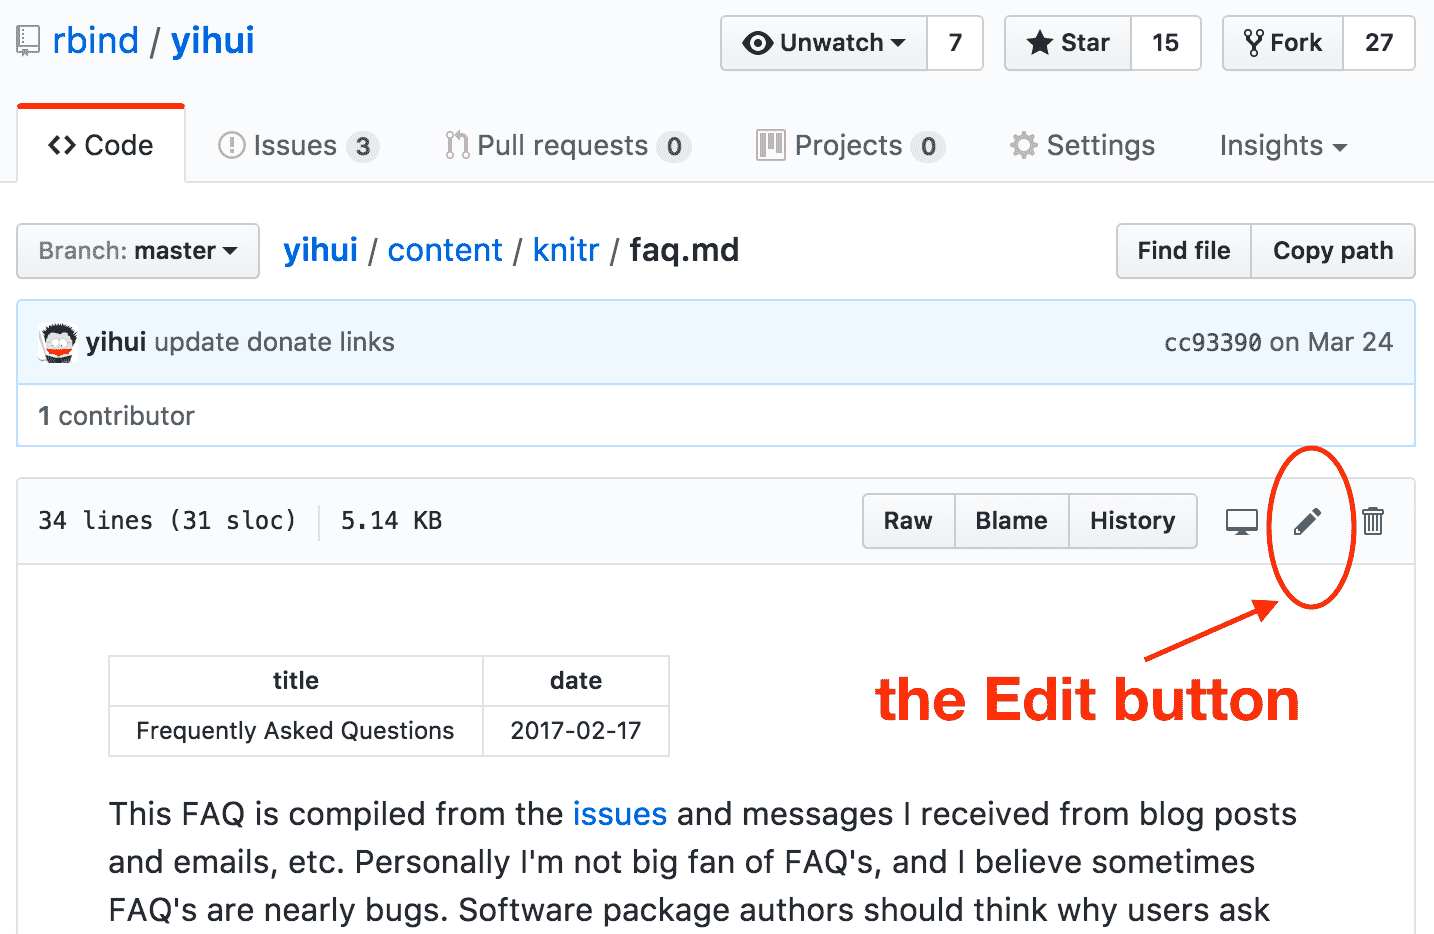
\includegraphics[width=1\linewidth]{images/github-edit} 

}

\caption{Edit a text file online on GitHub.}\label{fig:github-edit}
\end{figure}

After you digest the XMin theme and the implementations of additional
features, it should be much easier to understand other people's
templates. There are a large number of Hugo themes but the primary
differences among them are often in styles. The basic components of
templates are often similar.

\section{Custom layouts}\label{custom-layouts}

It is very likely that you want to customize a theme unless you designed
it. The most straightforward way is to simply make changes directly in
the theme,\footnote{If you are new to web development, be careful
  changing content within the theme. Minor changes like colors and font
  sizes can be found within the CSS files of the theme and can be
  altered simply with minimal risk of breaking the theme's
  functionality.} but the problem is that a Hugo theme may be constantly
updated by its original author for improvements or bug fixes. Similar to
the ``you break it, you buy it'' policy (the
\href{https://en.wikipedia.org/wiki/Pottery_Barn_rule}{Pottery Barn
rule}), once you touch someone else's source code, you will be
responsible for its future maintenance, and the original author should
not be responsible for the changes you made on your side. That means it
may not be easy to pull future updates of this theme to your website
(you have to carefully read the changes and make sure they do not
conflict with your changes), but if you are completely satisfied with
the current state of the theme and do not want future updates, it is
fine to modify the theme files directly.

A theme author who is aware of the fact that users may customize her
theme will typically provide two ways: one is to provide options in
\texttt{config.toml}, so that you can change these options without
touching the template files; the other is to leave a few lightweight
template files under \texttt{layouts/} in the theme, so that you can
override them without touching the core template files. Take the XMin
theme for example:

I have two empty HTML files \texttt{head\_custom.html} and
\texttt{foot\_custom.html} under \texttt{layouts/partials/} in the
theme. The former will be added inside
\texttt{\textless{}head\textgreater{}\textless{}/head\textgreater{}} of
a page, e.g., you can load JavaScript libraries or include CSS style
sheets via \texttt{\textless{}link\textgreater{}}. The latter will be
added before the footer of a page, e.g., you may load additional
JavaScript libraries or embed Disqus comments there.

The way that you customize these two files is not to edit them directly
in the theme folder, but to create a directory
\texttt{layouts/partials/} under the root directory of your website,
e.g., your directory structure may look like this:

\begin{Shaded}
\begin{Highlighting}[]
\ExtensionTok{your-website/}
\NormalTok{├── }\ExtensionTok{config.toml}
\NormalTok{├── }\ExtensionTok{...}
\NormalTok{├── }\ExtensionTok{themes/}
\NormalTok{│   └── }\ExtensionTok{hugo-xmin/}
\NormalTok{│       ├── }\ExtensionTok{...}
\NormalTok{│       └── }\ExtensionTok{layouts/}
\NormalTok{│           ├── }\ExtensionTok{...}
\NormalTok{│           └── }\ExtensionTok{partials}
\NormalTok{│               ├── }\ExtensionTok{foot_custom.html}
\NormalTok{│               ├── }\ExtensionTok{footer.html}
\NormalTok{│               ├── }\ExtensionTok{head_custom.html}
\NormalTok{│               └── }\ExtensionTok{header.html}
\NormalTok{└── }\ExtensionTok{layouts}
\NormalTok{    └── }\ExtensionTok{partials}
\NormalTok{        ├── }\ExtensionTok{foot_custom.html}
\NormalTok{        └── }\ExtensionTok{head_custom.html}
\end{Highlighting}
\end{Shaded}

All files under \texttt{layouts/} under the root directory will override
files with the same relative paths under
\texttt{themes/hugo-xmin/layouts/}, e.g., the file
\texttt{layouts/partials/foot\_custom.html}, when provided, will
override \texttt{themes/hugo-xmin/layouts/partials/foot\_custom.html}.
That means you only need to create and maintain at most two files under
\texttt{layouts/} instead of maintaining all files under
\texttt{themes/}. Note that this overriding mechanism applies to all
files under \texttt{layouts/}, and is not limited to the
\texttt{partials/} directory. It also applies to any Hugo theme that you
actually use for your website, and is not limited to \texttt{hugo-xmin}.

\section{Static files}\label{static-files}

All files under the \texttt{static/} directory\index{Static Directory}
are copied to \texttt{public/} when Hugo renders a website. This
directory is often used to store static web assets like images, CSS, and
JavaScript files. For example, an image \texttt{static/foo/bar.png} can
be embedded in your post using the Markdown syntax
\texttt{!{[}{]}(/foo/bar.png)}.\footnote{The link of the image depends
  on your \texttt{baseurl} setting in \texttt{config.toml}. If it does
  not contain a subpath, \texttt{/foo/bar.png} will be the link of the
  image, otherwise you may have to adjust it, e.g., for
  \texttt{baseurl\ =\ "http://example.com/subpath/"}, the link to the
  image should be \texttt{/subpath/foo/bar.png}.}

Usually a theme has a \texttt{static/} folder, and you can partially
override its files using the same mechanism as overriding
\texttt{layouts/} files, i.e., \texttt{static/file} will override
\texttt{themes/theme-name/static/file}. In the XMin theme, I have two
CSS files \texttt{style.css} and \texttt{fonts.css}. The former is the
main style sheet, and the latter is a quite small file to define
typefaces only. You may want to define your own typefaces, and you can
only provide a \texttt{static/css/fonts.css} to override the one in the
theme, e.g.,

\begin{Shaded}
\begin{Highlighting}[]
\NormalTok{body }\KeywordTok{\{}
  \KeywordTok{font-family:} \StringTok{"Comic Sans MS"}\NormalTok{, }\DataTypeTok{cursive}\NormalTok{, }\DataTypeTok{sans-serif}\KeywordTok{;}
\KeywordTok{\}}
\NormalTok{code }\KeywordTok{\{}
  \KeywordTok{font-family:} \StringTok{"Courier New"}\NormalTok{, Courier, }\DataTypeTok{monospace}\KeywordTok{;}
\KeywordTok{\}}
\end{Highlighting}
\end{Shaded}

To R Markdown users, another important application of the
\texttt{static/} directory is to build Rmd documents with custom output
formats, i.e., Rmd documents not using the
\texttt{blogdown::html\_page()} format (see Section
\ref{output-format}). For example, you can generate a PDF or
presentations from Rmd documents under this directory, so that Hugo will
not post-process them but simply copies them to \texttt{public/} for
publishing. To build these Rmd files, you must provide a custom build
script \texttt{R/build.R} (see Section \ref{methods}). You can write a
single line of code in this script\index{blogdown::build\_dir()}:

\begin{Shaded}
\begin{Highlighting}[]
\NormalTok{blogdown}\OperatorTok{::}\KeywordTok{build_dir}\NormalTok{(}\StringTok{"static"}\NormalTok{)}
\end{Highlighting}
\end{Shaded}

The function \texttt{build\_dir()} finds all Rmd files under a
directory, and calls \texttt{rmarkdown::render()} to build them to the
output formats specified in the YAML metadata of the Rmd files. If your
Rmd files should not be rendered by a simple
\texttt{rmarkdown::render()} call, you are free to provide your own code
to render them in \texttt{R/build.R}. There is a built-in caching
mechanism in the function \texttt{build\_dir()}: an Rmd file will not be
compiled if it is older than its output file(s). If you do not want this
behavior, you can force all Rmd files to be recompiled every time:
\texttt{build\_dir(force\ =\ TRUE)}.

I have provided a minimal example in the GitHub repository
\href{https://github.com/yihui/blogdown-static}{yihui/blogdown-static,}
where you can find two Rmd examples under the \texttt{static/}
directory. One is an HTML5 presentation based on the \textbf{xaringan}
package, and the other is a PDF document based on \textbf{bookdown}.

You need to be cautious about arbitrary files under \texttt{static/},
due to Hugo's overriding mechanism. That is, everything under
\texttt{static/} will be copied to \texttt{public/}. You need to make
sure that the files you render under \texttt{static/} will not conflict
with those files automatically generated by Hugo from \texttt{content/}.
For example, if you have a source file \texttt{content/about.md} and an
Rmd file \texttt{static/about/index.Rmd} at the same time, the HTML
output from the latter will overwrite the former (both Hugo and you will
generate an output file with the same name
\texttt{public/about/index.html}).

\chapter{Deployment}\label{deployment}

Since the website is basically a folder containing static files, it is
much easier to deploy than websites that require dynamic server-side
languages such as PHP or databases. All you need is to upload the files
to a server, and usually your website will be up and running shortly.
The key question is which web server you want to use. If you do not have
your own server, you may try the ones listed in this chapter. Most of
them are free (except Amazon S3), or at least provide free plans.
Disclaimer: the authors of this book are not affiliated with any of
these services or companies, and there is no guarantee that these
services will be provided forever.\footnote{You can easily find other
  similar services if you use your search engine.}

Considering the cost and friendliness to beginners, we currently
recommend Netlify (\url{https://www.netlify.com}). It provides a free
plan that actually has quite a lot of useful features. If you have no
experience in publishing websites before, just log in using your GitHub
account or other accounts, drag the \texttt{public/} folder built by
\textbf{blogdown} for your website to the Netlify page, and your website
will be online in a few seconds with a random subdomain name of the form
\texttt{random-word-12345.netlify.com} provided by Netlify (you can
customize the name). You can easily automate this process (see Section
\ref{netlify} for more details). You do not need to wrestle with
\texttt{ssh} or \texttt{rsync\ -zrvce} anymore, if you know what these
commands mean.

The second easiest solution may be Updog (\url{https://updog.co}), which
features Dropbox integration. Publishing a website can be as easy as
copying the files under the \texttt{public/} folder of your
\textbf{blogdown} website to a Dropbox folder. The free plan of Updog
only provides limited features, and its paid plan will give you access
to much richer features.

If you do not mind using command-line tools or are familiar with
GIT/GitHub, you can certainly consider services like GitHub Pages,
Travis CI, or Amazon S3 to build or host your websites. No matter which
service you use, please keep in mind that none of them can really lock
you in and you are always free to change the service. As we have
mentioned before, one great advantage of \textbf{blogdown} is that your
website will be a folder of static files that you can move to any web
server.

\section{Netlify}\label{netlify}

As we just mentioned, Netlify\index{Netlify} allows you to quickly
publish a website by uploading the \texttt{public/} folder through its
web interface, and you will be assigned a random subdomain
\texttt{*.netlify.com}.\footnote{You don't have to keep the
  \texttt{*.netlify.com} domain. See Appendix \ref{domain-name} for more
  information.} This approach is good for those websites that are not
updated frequently (or at all). However, it is unlikely that you will
not need to update your website, so we introduce a better approach in
this section,\footnote{Please bear in mind that the purpose of this
  section is to outline the basic steps of publishing a website with
  Netlify, and the technical details may change from time to time, so
  the official Netlify documentation should be the most reliable source
  if you have any questions or anything we introduced here does not
  work.} which will take you a few more minutes to complete the
configurations. Once it is properly configured, all you need to do in
the future is to update the source repository, and Netlify will call
Hugo to render your website automatically.

Basically, you have to host all source files of your website in a GIT
repository.\footnote{If the contents of your \texttt{blogdown} site are
  not in the root directory of your GIT repository, Netlify will not
  build.} You do not need to put the \texttt{public/} directory under
version control\footnote{You can add \texttt{public} to
  \texttt{.gitignore} to ignore it in GIT.} because it will be
automatically generated. Currently, Netlify supports GIT repositories
hosted on GitHub, GitLab, and BitBucket. With any of these accounts, you
can log into Netlify from its homepage and follow the guide to create a
new site from your GIT repository.

Netlify supports several static website generators, including Jekyll and
Hugo. For a new site, you have to specify a command to build your
website, as well as the path of the publish directory. Netlify also
supports multiple versions of Hugo, so the build command can be the
default \texttt{hugo}. The default version is 0.17, which is too old,
and we recommend that you use at least version 0.20. To specify a Hugo
version greater or equal to 0.20, you need to create an environment
variable \texttt{HUGO\_VERSION} on Netlify. See the
\href{https://www.netlify.com/docs/continuous-deployment/}{Netlify
documentation} for more information. The publish directory should be
\texttt{public} unless you have changed it in your \texttt{config.toml}.
Figure \ref{fig:netlify-settings} shows the settings of the website
\url{https://t.yihui.name}. You do not have to follow the exact settings
for your own website; in particular, you may need to change the value of
the environment variable \texttt{HUGO\_VERSION} to a recent version of
Hugo.\footnote{By the time when this book is published, the version
  0.24.1 may be too old.}

\begin{figure}

{\centering 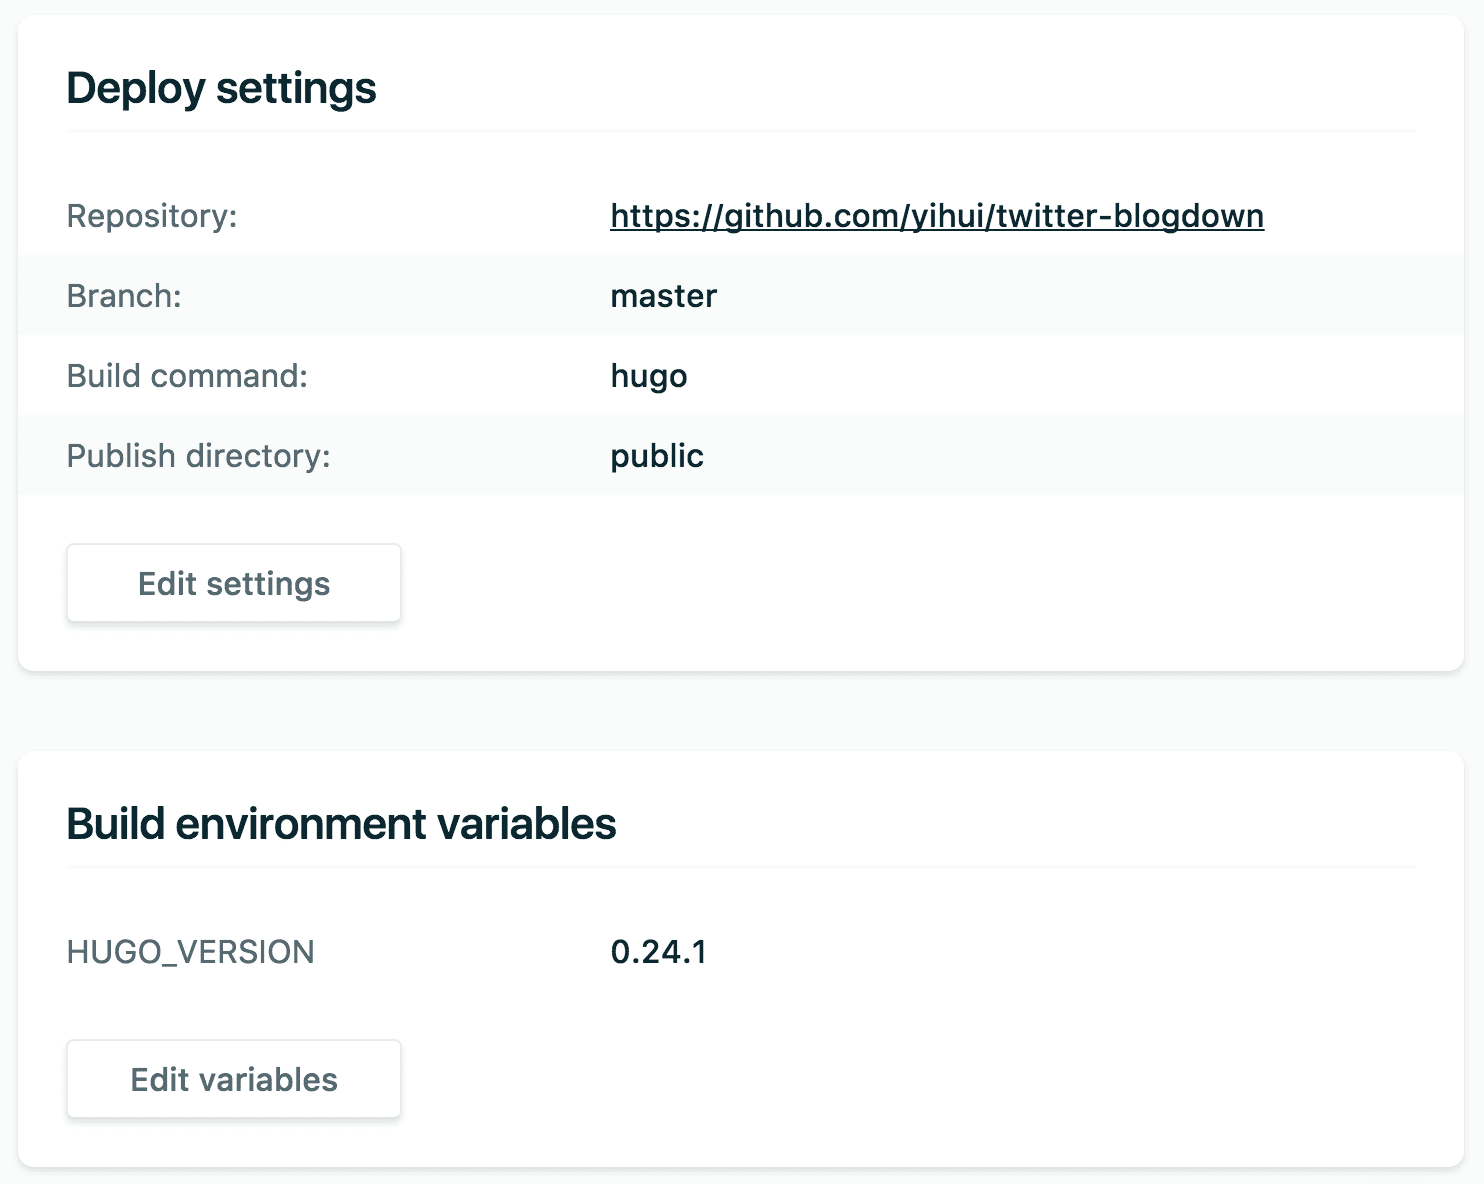
\includegraphics[width=1\linewidth]{images/netlify-settings} 

}

\caption{Example settings of a website deployed on Netlify.}\label{fig:netlify-settings}
\end{figure}

It may take a minute or two to deploy your website on Netlify for the
first time, but it can be much faster later (a few seconds) when you
update your website source, because Netlify deploys incremental changes
in the \texttt{public/} directory, i.e., only the newer files compared
to the last time are deployed.

After your GIT repository is connected with Netlify, the last issue you
may want to solve is the domain name\index{Domain Name}, unless you are
satisfied with the free Netlify subdomain. If you want to use a
different domain, you need to configure some DNS records of the domain
to point it to the Netlify server. See Appendix \ref{domain-name} for
some background knowledge on domain names.

If you are not familiar with domain names or do not want to learn more
about them, something to consider is a free subdomain
\texttt{*.rbind.io} offered by RStudio, Inc. Please visit the Rbind
support website \url{https://support.rbind.io} to learn how to apply for
a subdomain. In fact, the Rbind organization also offers free help on
how to set up a website based on \textbf{blogdown}, thanks to a lot of
volunteers from the R and statistics community.

Netlify is the only solution in this chapter that does not require you
to prebuild your website. You only need to update the source files, push
them to GitHub, and Netlify will build the website for you.\footnote{This
  is called ``continuous deployment.''} The rest of the solutions in
this chapter will require you to build your website locally and upload
the \texttt{public/} folder explicitly or implicitly. That said, you can
certainly prebuild your website using any tools, push it to GitHub, and
Netlify is still able to deploy it for you. What you need to do is leave
the build command empty, and tell Netlify your publish directory (e.g.,
Hugo's default \texttt{public/}, but if your prebuilt website is under
the root directory, specify \texttt{.} as the publish directory
instead). Then Netlify simply uploads all files under this directory to
its servers without rebuilding your website.

\section{Updog}\label{updog}

Updog (\url{https://updog.co}) provides\index{Updog} a simple service:
it turns a specified Dropbox (or Google Drive) folder into a website.
The idea is that you grant Updog the permission to read the folder, and
it will act as a middleman to serve your files under this folder to your
visitors. This folder has to be accessed via a domain name, and Updog
offers a free subdomain \texttt{*.updog.co}. For example, if you have
assigned the domain \texttt{example.updog.co} to your Dropbox folder,
and a visitor wants to see the page
\texttt{https://example.updog.co/foo/index.html}, Updog will read the
file \texttt{foo/index.html} in your Dropbox folder and display it to
the visitor.

At the moment, Updog's free plan only allows one website per account and
will insert a footer ``Hosted on Updog'' on your web pages. You may not
like these limitations. The major benefit of using Updog is that
publishing a website becomes implicit since Dropbox will continuously
sync files. All you need to do is to make sure your website is generated
to the correct Dropbox folder. This can be easily achieved by setting
the option \texttt{publishDir} in \texttt{config.toml}. For example,
suppose the folder that you assign to Updog is
\texttt{\textasciitilde{}/Dropbox/Apps/updog/my-website/}, and your
source folder is at
\texttt{\textasciitilde{}/Dropbox/Apps/updog/my-source/}, then you can
set \texttt{publishDir:\ "../my-website"} in
\texttt{\textasciitilde{}/Dropbox/Apps/updog/my-source/config.toml}.

You can also use your custom domain name if you do not want the default
Updog subdomain, and you only need to point the CNAME record of your
domain name to the Updog subdomain.\footnote{See Appendix
  \ref{domain-name} for more information.}

\section{GitHub Pages}\label{github-pages}

GitHub Pages (\url{https://pages.github.com}) \index{GitHub Pages} is a
very popular way to host static websites (especially those built with
Jekyll), but its advantages are not obvious or appealing compared to
Netlify. We recommend that you consider Netlify + Hugo due to these
reasons:

\begin{itemize}
\item
  Currently, GitHub Pages does not support HTTPS for custom domain
  names. HTTPS only works for \texttt{*.github.io} subdomains. This
  limitation does not exist on Netlify. You may read the article
  \href{https://https.cio.gov/everything/}{``Why HTTPS for
  Everything?''} to understand why it is important, and you are
  encouraged to turn on HTTPS for your website whenever you can.
\item
  Redirecting URLs is awkward with GitHub Pages but much more
  straightforward with Netlify.\footnote{GitHub Pages uses a Jekyll
    plugin to write an \texttt{HTTP-REFRESH} meta tag to redirect pages,
    and Netlify can do pattern-based 301 or 302 redirects, which can
    notify search engines that certain pages have been moved
    (permanently or temporarily).} This is important especially when you
  have an old website that you want to migrate to Hugo; some links may
  be broken, in which case you can easily redirect them with Netlify.
\item
  One of the best features of Netlify that is not available with GitHub
  Pages is that Netlify can generate a unique website for preview when a
  GitHub pull request is submitted to your GitHub repository. This is
  extremely useful when someone else (or even yourself) proposes changes
  to your website, since you have a chance to see what the website would
  look like before you merge the pull request.
\end{itemize}

Basically, Netlify can do everything that GitHub Pages can, but there is
still one little missing feature, which is closely tied to GitHub
itself, which is GitHub
\href{https://help.github.com/articles/user-organization-and-project-pages/}{Project
Pages.} This feature allows you to have project websites in separate
repositories, e.g., you may have two independent websites
\texttt{https://username.github.io/proj-a/} and
\texttt{https://username.github.io/proj-b/}, corresponding to GitHub
repositories \texttt{username/proj-a} and \texttt{username/proj-b},
respectively. However, since you can connect any GitHub repositories
with Netlify, and each repository can be associated with a domain or
subdomain name, you may replace GitHub Project Pages with different
subdomains like \texttt{proj-a.netlify.com} and
\texttt{proj-b.netlify.com}. The actual limitation is that you cannot
use subpaths in the URL but you can use any (sub)domain names.

Although GitHub does not officially support Hugo (only Jekyll is
supported), you can actually publish any static HTML files on GitHub
Pages, even if they are not built with Jekyll. The first requirement for
using GitHub Pages is that you have to create a GitHub repository named
\texttt{username.github.io} under your account (replace
\texttt{username} with your actual GitHub username), and what's left is
to push your website files to this repository. The comprehensive
documentation of GitHub Pages is at \url{https://pages.github.com}, and
please ignore anything related to Jekyll there unless you actually use
Jekyll instead of Hugo. To make sure GitHub does not rebuild your
website using Jekyll and just publish whatever files you push to the
repository, you need to create a (hidden) file named \texttt{.nojekyll}
in the repository.\footnote{You may use the R function
  \texttt{file.create(\textquotesingle{}.nojekyll\textquotesingle{})} to
  create this file if you do not know how to do this.} GitHub offers a
free subdomain \texttt{username.github.io}, and you can use your own
domain name by configuring its A or CNAME records to point it to GitHub
Pages (consult the GitHub Pages documentation for instructions).

Your \texttt{public/} directory should be the GIT repository. You have
two possible choices for setting up this repository locally. The first
choice is to follow the default structure of a Hugo website like the
diagram below, and initialize the GIT repository under the
\texttt{public/} directory:

\begin{Shaded}
\begin{Highlighting}[]
\ExtensionTok{source/}
\NormalTok{│}
\NormalTok{├── }\ExtensionTok{config.toml}
\NormalTok{├── }\ExtensionTok{content/}
\NormalTok{├── }\ExtensionTok{themes/}
\NormalTok{├── }\ExtensionTok{...}
\NormalTok{└── }\ExtensionTok{public/}
    \KeywordTok{|}
\NormalTok{    ├── }\ExtensionTok{.git/}
\NormalTok{    ├── }\ExtensionTok{.nojekyll}
\NormalTok{    ├── }\ExtensionTok{index.html}
\NormalTok{    ├── }\ExtensionTok{about/}
\NormalTok{    └── }\ExtensionTok{...}
\end{Highlighting}
\end{Shaded}

If you know how to use the command line, change the working directory to
\texttt{public/}, and initialize the GIT repository there:

\begin{Shaded}
\begin{Highlighting}[]
\BuiltInTok{cd}\NormalTok{ public}
\FunctionTok{git}\NormalTok{ init}
\FunctionTok{git}\NormalTok{ remote add origin https://github.com/username/username.github.io}
\end{Highlighting}
\end{Shaded}

The other choice is to clone the GitHub repository you created to the
same directory as your website source:

\begin{Shaded}
\begin{Highlighting}[]
\FunctionTok{git}\NormalTok{ clone https://github.com/username/username.github.io}
\end{Highlighting}
\end{Shaded}

And the structure looks like this:

\begin{Shaded}
\begin{Highlighting}[]
\ExtensionTok{source/}
\NormalTok{│}
\NormalTok{├── }\ExtensionTok{config.toml}
\NormalTok{├── }\ExtensionTok{content/}
\NormalTok{├── }\ExtensionTok{themes/}
\NormalTok{└── }\ExtensionTok{...}

\ExtensionTok{username.github.io/}
\NormalTok{│}
\NormalTok{├── }\ExtensionTok{.git/}
\NormalTok{├── }\ExtensionTok{.nojekyll}
\NormalTok{├── }\ExtensionTok{index.html}
\NormalTok{├── }\ExtensionTok{about/}
\NormalTok{└── }\ExtensionTok{...}
\end{Highlighting}
\end{Shaded}

The source directory and the \texttt{username.github.io} directory are
under the same parent directory. In this case, you need to set the
option \texttt{publishDir:\ "../username.github.io"} in
\texttt{source/config.toml}.

\section{Travis + GitHub}\label{travis-github}

If \index{Travis CI} you decide not to follow our recommendation to use
Netlify to deploy your website, we should warn you that the approach in
this section will require substantial knowledge about GIT, GitHub,
Travis CI (\url{https://travis-ci.org}), and the Linux command line,
which we will leave for you to learn on your own. The major advantage of
publishing via Travis CI is that you can compile all your Rmd posts on
Travis CI (on the cloud) instead of your local computer.

In case you are not familiar with Travis, it is a service to
continuously check your software in a virtual machine whenever you push
changes to GitHub. It is primarily for testing software, but since you
can run a lot of commands in its virtual machine, you can certainly use
the virtual machine to do other things, e.g., install R and the
\textbf{blogdown} package to build websites. Before I show you how, I'd
like to mention two issues that you should be aware of:

\begin{itemize}
\item
  Personally, I prefer taking a look at the output in GIT to see the
  changes when I have any output that is dynamically computed from R, so
  that I know for sure what I'm going to publish exactly. With Travis,
  it is somewhat unpredictable because it is fully automatic and you do
  not have a chance to see the new content or results to be published.
  There are many factors that could affect building the site: the R
  version, availability of certain R packages, system dependencies, and
  network connection, etc.
\item
  The time required to compile all Rmd files may be very long and cause
  timeouts on Travis, depending on how time-consuming your R code is.
  There is a caching mechanism in \textbf{blogdown} to speed up the
  building of your site (see Section \ref{methods}), and if you use
  Travis to build your website, you will not benefit from this caching
  mechanism unless you take advantage of Travis's caching. You have to
  cache the directories \texttt{content/}, \texttt{static/}, and
  \texttt{blogdown/}, but Travis's cache is a little fragile in my
  experience. Sometimes the cache may be purged for unknown reasons.
  What is more, you cannot directly cache \texttt{content/} and
  \texttt{static/}, because Travis clones your repository before
  restoring the cache, which means old files from the cached
  \texttt{content/} and \texttt{static/} may overwrite new files you
  pushed to GitHub.
\end{itemize}

The second problem can be solved, but I do not want to explain how in
this book since the solution is too involved. If you really want to use
Travis to build your website and run into this problem, you may file an
issue to the GitHub repository
\url{https://github.com/yihui/travis-blogdown}. In fact, this repository
is a minimal example I created to show how to build a website on Travis
and publish to GitHub Pages.

The Travis documentation shows how to deploy a site to GitHub Pages:
\url{https://docs.travis-ci.com/user/deployment/pages/}, but does not
show how to build a site. Here is the Travis configuration file,
\texttt{.travis.yml}, for the \texttt{travis-blogdown} repository:

\begin{Shaded}
\begin{Highlighting}[]
\FunctionTok{language:}\AttributeTok{ r}
\FunctionTok{dist:}\AttributeTok{ trusty}
\FunctionTok{sudo:}\AttributeTok{ false}

\FunctionTok{branches:}
  \FunctionTok{only:}
    \KeywordTok{-}\NormalTok{ master}

\FunctionTok{cache:}
  \FunctionTok{packages:}\AttributeTok{ yes}
  \FunctionTok{directories:}
    \KeywordTok{-}\NormalTok{ $HOME/bin}

\FunctionTok{before_script:}
  \KeywordTok{-} \StringTok{"Rscript -e 'blogdown::install_hugo()'"}

\FunctionTok{script:}
  \KeywordTok{-} \StringTok{"Rscript -e 'blogdown::build_site()'"}

\FunctionTok{deploy:}
  \FunctionTok{provider:}\AttributeTok{ pages}
  \FunctionTok{skip_cleanup:}\AttributeTok{ true}
  \FunctionTok{github_token:}\AttributeTok{ $GITHUB_TOKEN}
  \FunctionTok{on:}
    \FunctionTok{branch:}\AttributeTok{ master}
  \FunctionTok{local_dir:}\AttributeTok{ public}
  \FunctionTok{fqdn:}\AttributeTok{ travis-blogdown.yihui.name}
\end{Highlighting}
\end{Shaded}

The key is that we install Hugo via \texttt{blogdown::install\_hugo()}
and build the site via \texttt{blogdown::build\_site()}. To trick Travis
into building this repository like an R package, you must have a
\texttt{DESCRIPTION} file in the repository, otherwise your website will
not be built.

\begin{Shaded}
\begin{Highlighting}[]
\FunctionTok{Package:}\AttributeTok{ placeholder}
\FunctionTok{Type:}\AttributeTok{ Website}
\FunctionTok{Title:}\AttributeTok{ Does not matter.}
\FunctionTok{Version:}\AttributeTok{ 0.0.1}
\FunctionTok{Imports:}\AttributeTok{ blogdown}
\FunctionTok{Remotes:}\AttributeTok{ rstudio/blogdown}
\end{Highlighting}
\end{Shaded}

There are a few more things to explain and emphasize in
\texttt{.travis.yml}:

\begin{itemize}
\item
  The \texttt{branches} option specifies that only changes in the
  \texttt{master} branch will trigger building on Travis.
\item
  The \texttt{cache} option specifies all R packages to be cached, so
  the next time it will be faster to build the site (R packages do not
  need to be reinstalled from source). The \texttt{bin/} directory in
  the home directory is also cached because Hugo is installed there, and
  the next time Hugo does not need to be reinstalled.
\item
  For the \texttt{deploy} option, there is an environment variable named
  \texttt{GITHUB\_TOKEN}, and I have specified its value to be a GitHub
  personal access token via the Travis settings of this repository, so
  that Travis will be able to write to my repository after the website
  is built. The option \texttt{on} specifies that the deployment will
  only occur when the \texttt{master} branch is built. The
  \texttt{local\_dir} option is the publish directory, which should
  default to \texttt{public} in Hugo. By default, the website is pushed
  to the \texttt{gh-pages} branch of this repository. The \texttt{fqdn}
  option specifies the custom domain of the website. I have set a CNAME
  record (see Appendix \ref{domain-name}) to point
  \texttt{travis-blogdown.yihui.name} to \texttt{yihui.github.io}, so
  that GitHub is able to serve this website through this domain (in
  fact, Travis will write a \texttt{CNAME} file containing the domain to
  the \texttt{gh-pages} branch).
\end{itemize}

If you use the \texttt{username.github.io} repository on GitHub, the
website must be pushed to its \texttt{master} branch instead of
\texttt{gh-pages} (this is the only exception). I recommend that you
separate the source repository and the output repository. For example,
you may have a \texttt{website-source} repository with the same settings
as the above \texttt{.travis.yml} except for two new options under
\texttt{deploy}:

\begin{Shaded}
\begin{Highlighting}[]
\FunctionTok{deploy:}
\NormalTok{  ...}
  \FunctionTok{repo:}\AttributeTok{ username/username.github.io}
  \FunctionTok{target_branch:}\AttributeTok{ master}
\end{Highlighting}
\end{Shaded}

This means the website will be pushed to the \texttt{master} branch of
the repository \texttt{username/username.github.io} (remember to replace
\texttt{username} with your actual username).

You can also deploy your website to Amazon S3\index{Amazon S3}, and the
setup on the R side is very similar to what we have introduced for
GitHub Pages. The only difference is in the last step, where you change
the target from GitHub Pages to Amazon S3. For more information, please
see the documentation on Travis:
\url{https://docs.travis-ci.com/user/deployment/s3/}.

\section{GitLab Pages}\label{gitlab-pages}

GitLab (\url{http://gitlab.com}) is a very popular way to host the
source code of your project. GitLab has a
\href{https://about.gitlab.com/features/gitlab-ci-cd/}{built in
Continuous Integration \& Deployment (CI/CD) service} that can be used
to host static websites, named
\href{https://about.gitlab.com/features/pages/}{GitLab Pages}. The major
advantage of using GitLab Pages is that you will be able to compile all
your Rmd posts through its CI/CD service instead of your local computer
and any generated content, such as HTML files, will be automatically
copied to the web server. Please note that this approach has similar
issues as the Travis + GitHub approach in Section \ref{travis-github}.

GitLab's CI/CD service uses the instructions stored in the YAML file
\texttt{.gitlab-ci.yml} in the repository. Here is a sample
configuration file \texttt{.gitlab-ci.yml} from the example repository
\url{https://gitlab.com/rgaiacs/blogdown-gitlab}:

\begin{Shaded}
\begin{Highlighting}[]
\FunctionTok{image:}\AttributeTok{ debian:buster-slim}

\FunctionTok{before_script:}
  \KeywordTok{-}\NormalTok{ apt-get update && apt-get -y install pandoc r-base}
  \KeywordTok{-} \FunctionTok{R -e "install.packages('blogdown',repos='http:}\AttributeTok{//cran.rstudio.com')"}
  \KeywordTok{-} \FunctionTok{R -e "blogdown:}\AttributeTok{:install_hugo()"}

\FunctionTok{pages:}
  \FunctionTok{script:}
    \KeywordTok{-} \FunctionTok{R -e "blogdown:}\AttributeTok{:build_site()"}
  \FunctionTok{artifacts:}
    \FunctionTok{paths:}
      \KeywordTok{-}\NormalTok{ public}
  \FunctionTok{only:}
    \KeywordTok{-}\NormalTok{ master}
\end{Highlighting}
\end{Shaded}

The \texttt{image} option specifies what
\href{https://www.docker.com}{Docker} image will be use as a start
point. We are using a Debian image but any image from
\href{https://hub.docker.com/}{Docker Hub} can be used. Other settings
and options are similar to \texttt{.travis.yml} in Section
\ref{travis-github}. The above example generates the website at
\url{https://rgaiacs.gitlab.io/blogdown-gitlab}.

\chapter{Migration}\label{migration}

Usually, it is easier to start a new website than
migrating\index{Site Migration} an old one to a new framework, but you
may have to do it anyway because of the useful content on the old
website that should not simply be discarded. A lazy solution is to leave
the old website as is, start a new website with a new domain, and
provide a link to the old website. This may be a hassle to your readers,
and they may not be able to easily discover the gems that you created on
your old website, so I recommend that you migrate your old posts and
pages to the new website if possible.

This process may be easy or hard, depending on how complicated your old
website is. The bad news is that there is unlikely to be a universal or
magical solution, but I have provided some helper functions in
\textbf{blogdown} as well as a Shiny application to assist you, which
may make it a little easier for you to migrate from Jekyll and WordPress
sites.

To give you an idea about the possible amount of work required, I can
tell you that it took me a whole week (from the morning to midnight
every day) to migrate several of my personal Jekyll-based websites to
Hugo and \textbf{blogdown}. The complication in my case was not only
Jekyll, but also the fact that I built several separate Jekyll websites
(because I did not have a choice in Jekyll) and I wanted to unite them
in the same repository. Now my two blogs (Chinese and English), the
\textbf{knitr} \citep{R-knitr} package documentation, and the
\textbf{animation} package \citep{R-animation} documentation are
maintained in the same repository: \url{https://github.com/rbind/yihui}.
I have about 1000 pages on this website, most of which are blog posts.
It used to take me more than 30 seconds to preview my blog in Jekyll,
and now it takes less than 2 seconds to build the site in Hugo.

Another complicated example is the website of Rob J Hyndman
(\url{https://robjhyndman.com}). He started his website in 1993 (12
years before me), and had accumulated a lot of content over the years.
You can read the post
\url{https://support.rbind.io/2017/05/15/converting-robjhyndman-to-blogdown/}
for the stories about how he migrated his WordPress website to
\textbf{blogdown}. The key is that you probably need a long
international flight when you want to migrate a complicated website.

A simpler example is the Simply Statistics blog
(\url{https://simplystatistics.org}). Originally it was built on
Jekyll\footnote{It was migrated from WordPress a few years ago. The
  WordPress site was actually migrated from an earlier Tumblr blog.} and
the source was hosted in the GitHub repository
\url{https://github.com/simplystats/simplystats.github.io}. I
volunteered to help them move to \textbf{blogdown}, and it took me about
four hours. My time was mostly spent on cleaning up the YAML metadata of
posts and tweaking the Hugo theme. They had about 1000 posts, which
sounds like a lot, but the number does not really matter, because I
wrote an R script to process all posts automatically. The new repository
is at \url{https://github.com/rbind/simplystats}.

If you do not really have too many pages (e.g., under 20), I recommend
that you cut and paste them to Markdown files, because it may actually
take longer to write a script to process these pages.

It is likely that some links will be broken after the migration because
Hugo renders different links for your pages and posts. In that case, you
may either fix the permanent links (e.g., by tweaking the slug of a
post), or use 301 redirects (e.g., on Netlify).

\section{From Jekyll}\label{from-jekyll}

When converting a Jekyll\index{Jekyll} website to Hugo, the most
challenging part is the theme. If you want to keep exactly the same
theme, you will have to rewrite your Jekyll templates using Hugo's
syntax (see Section \ref{templates}). However, if you can find an
existing theme in Hugo (\url{https://themes.gohugo.io}), things will be
much easier, and you only need to move the content of your website to
Hugo, which is relatively easy. Basically, you copy the Markdown pages
and posts to the \texttt{content/} directory in Hugo and tweak these
text files.

Usually, posts in Jekyll are under the \texttt{\_posts/} directory, and
you can move them to \texttt{content/post/} (you are free to use other
directories). Then you need to define a custom rule for permanent URLs
in \texttt{config.toml} like (see Section \ref{options}):

\begin{Shaded}
\begin{Highlighting}[]
\NormalTok{[permalinks]}
\NormalTok{    post }\OperatorTok{=} \StringTok{"/:year/:month/:day/:slug/"}
\end{Highlighting}
\end{Shaded}

This depends on the format of the URLs you used in Jekyll (see the
\texttt{permalink} option in your \texttt{\_config.yml}).

If there are static assets like images, they can be moved to the
\texttt{static/} directory in Hugo.

Then you need to use your favorite tool with some string manipulation
techniques to process all Markdown files. If you use R, you can list all
Markdown files and process them one by one in a loop. Below is a sketch
of the code:

\begin{Shaded}
\begin{Highlighting}[]
\NormalTok{files =}\StringTok{ }\KeywordTok{list.files}\NormalTok{(}
  \StringTok{'content/'}\NormalTok{, }\StringTok{'[.](md|markdown)$'}\NormalTok{, }\DataTypeTok{full.names =} \OtherTok{TRUE}\NormalTok{,}
  \DataTypeTok{recursive =} \OtherTok{TRUE}
\NormalTok{)}
\ControlFlowTok{for}\NormalTok{ (f }\ControlFlowTok{in}\NormalTok{ files) \{}
\NormalTok{  blogdown}\OperatorTok{:::}\KeywordTok{process_file}\NormalTok{(f, }\ControlFlowTok{function}\NormalTok{(x) \{}
    \CommentTok{# process x here and return the modified x}
\NormalTok{    x}
\NormalTok{  \})}
\NormalTok{\}}
\end{Highlighting}
\end{Shaded}

The \texttt{process\_file()} function is an internal helper function in
\textbf{blogdown}. It takes a filename and a processor function to
manipulate the content of the file, and writes the modified text back to
the file.

To give you an idea of what a processor function may look like, I
provided a few simple helper functions in \textbf{blogdown}, and below
are two of them:

\begin{Shaded}
\begin{Highlighting}[]
\NormalTok{blogdown}\OperatorTok{:::}\NormalTok{remove_extra_empty_lines}
\end{Highlighting}
\end{Shaded}

\begin{verbatim}
function (f) 
process_file(f, function(x) {
    x = paste(gsub("\\s+$", "", x), collapse = "\n")
    trim_ws(gsub("\n{3,}", "\n\n", x))
})
<environment: namespace:blogdown>
\end{verbatim}

\begin{Shaded}
\begin{Highlighting}[]
\NormalTok{blogdown}\OperatorTok{:::}\NormalTok{process_bare_urls}
\end{Highlighting}
\end{Shaded}

\begin{verbatim}
function (f) 
process_file(f, function(x) {
    gsub("\\[([^]]+)]\\(\\1/?\\)", "<\\1>", x)
})
<environment: namespace:blogdown>
\end{verbatim}

The first function substitutes two or more empty lines with a single
empty line. The second function replaces links of the form
\texttt{{[}url{]}(url)} with \texttt{\textless{}url\textgreater{}}.
There is nothing wrong with excessive empty lines or the syntax
\texttt{{[}url{]}(url)}, though. These helper functions may make your
Markdown text a little cleaner. You can find all such helper functions
at \url{https://github.com/rstudio/blogdown/blob/master/R/clean.R}. Note
they are not exported from \textbf{blogdown}, so you need triple colons
to access them.

The YAML metadata of your posts may not be completely clean, especially
when your Jekyll website was actually converted from an earlier
WordPress website. The internal helper function
\texttt{blogdown:::modify\_yaml()} may help you clean up the metadata.
For example, below is the YAML metadata of a blog post of Simply
Statistics when it was built on Jekyll:

\begin{Shaded}
\begin{Highlighting}[]
\OtherTok{---}
\FunctionTok{id:}\AttributeTok{ 4155}
\FunctionTok{title:}\AttributeTok{ Announcing the JHU Data Science Hackathon 2015}
\FunctionTok{date:}\AttributeTok{ 2015-07-28T13:31:04+00:00}
\FunctionTok{author:}\AttributeTok{ Roger Peng}
\FunctionTok{layout:}\AttributeTok{ post}
\FunctionTok{guid:}\AttributeTok{ http://simplystatistics.org/?p=4155}
\FunctionTok{permalink:}\AttributeTok{ /2015/07/28/announcing-the-jhu-data-science-hackathon-2015}
\FunctionTok{pe_theme_meta:}
  \KeywordTok{-} \StringTok{'O:8:"stdClass":2:\{s:7:"gallery";O:8:"stdClass":...\}'}
\FunctionTok{al2fb_facebook_link_id:}
  \KeywordTok{-}\NormalTok{ 136171103105421_837886222933902}
\FunctionTok{al2fb_facebook_link_time:}
  \KeywordTok{-} \FunctionTok{2015-07-28T17:}\AttributeTok{31:11+00:00}
\FunctionTok{al2fb_facebook_link_picture:}
  \KeywordTok{-} \FunctionTok{post=http:}\AttributeTok{//simplystatistics.org/?al2fb_image=1}
\FunctionTok{dsq_thread_id:}
  \KeywordTok{-}\NormalTok{ 3980278933}
\FunctionTok{categories:}
  \KeywordTok{-}\NormalTok{ Uncategorized}
\OtherTok{---}
\end{Highlighting}
\end{Shaded}

You can discard the YAML fields that are not useful in Hugo. For
example, you may only keep the fields \texttt{title}, \texttt{author},
\texttt{date}, \texttt{categories}, and \texttt{tags}, and discard other
fields. Actually, you may also want to add a \texttt{slug} field that
takes the base filename of the post (with the leading date removed). For
example, when the post filename is
\texttt{2015-07-28-announcing-the-jhu-data-science-hackathon-2015.md},
you may want to add
\texttt{slug:\ announcing-the-jhu-data-science-hackathon-2015} to make
sure the URL of the post on the new site remains the same.

Here is the code to process the YAML metadata of all posts:

\begin{Shaded}
\begin{Highlighting}[]
\ControlFlowTok{for}\NormalTok{ (f }\ControlFlowTok{in}\NormalTok{ files) \{}
\NormalTok{  blogdown}\OperatorTok{:::}\KeywordTok{modify_yaml}\NormalTok{(f, }\DataTypeTok{slug =} \ControlFlowTok{function}\NormalTok{(old, yaml) \{}
    \CommentTok{# YYYY-mm-dd-name.md -> name}
    \KeywordTok{gsub}\NormalTok{(}\StringTok{'^}\CharTok{\textbackslash{}\textbackslash{}}\StringTok{d\{4\}-}\CharTok{\textbackslash{}\textbackslash{}}\StringTok{d\{2\}-}\CharTok{\textbackslash{}\textbackslash{}}\StringTok{d\{2\}-|[.](md|markdown)'}\NormalTok{, }\StringTok{''}\NormalTok{, f)}
\NormalTok{  \}, }\DataTypeTok{categories =} \ControlFlowTok{function}\NormalTok{(old, yaml) \{}
    \CommentTok{# remove the Uncategorized category}
    \KeywordTok{setdiff}\NormalTok{(old, }\StringTok{'Uncategorized'}\NormalTok{)}
\NormalTok{  \}, }\DataTypeTok{.keep_fields =} \KeywordTok{c}\NormalTok{(}
    \StringTok{'title'}\NormalTok{, }\StringTok{'author'}\NormalTok{, }\StringTok{'date'}\NormalTok{, }\StringTok{'categories'}\NormalTok{, }\StringTok{'tags'}\NormalTok{, }\StringTok{'slug'}
\NormalTok{  ), }\DataTypeTok{.keep_empty =} \OtherTok{FALSE}\NormalTok{)}
\NormalTok{\}}
\end{Highlighting}
\end{Shaded}

You can pass a file path to \texttt{modify\_yaml()}, define new YAML
values (or functions to return new values based on the old values), and
decide which fields to preserve (\texttt{.keep\_fields}). You may
discard empty fields via \texttt{.keep\_empty\ =\ FALSE}. The processed
YAML metadata is below, which looks much cleaner:

\begin{Shaded}
\begin{Highlighting}[]
\OtherTok{---}
\FunctionTok{title:}\AttributeTok{ Announcing the JHU Data Science Hackathon 2015}
\FunctionTok{author:}\AttributeTok{ Roger Peng}
\FunctionTok{date:}\AttributeTok{ }\StringTok{'2015-07-28T13:31:04+00:00'}
\FunctionTok{slug:}\AttributeTok{ announcing-the-jhu-data-science-hackathon-2015}
\OtherTok{---}
\end{Highlighting}
\end{Shaded}

\section{From WordPress}\label{from-wordpress}

From our experience, the best way to import WordPress\index{WordPress}
blog posts to Hugo is to import them to Jekyll, and write an R script to
clean up the YAML metadata of all pages if necessary, instead of using
the migration tools listed on the
\href{https://gohugo.io/tools/}{official guide,} including the WordPress
plugin \texttt{wordpress-to-hugo-exporter}.

To our knowledge, the best tool to convert a WordPress website to Jekyll
is the Python tool \href{https://github.com/thomasf/exitwp}{Exitwp.} Its
author has provided detailed instructions on how to use it. You have to
know how to install Python libraries and execute Python scripts. If you
do not, I have provided an online tool at
\url{https://github.com/yihui/travis-exitwp}. You can upload your
WordPress XML file there, and get a download link to a ZIP archive that
contains your posts in Markdown.

The biggest challenge in converting WordPress posts to Hugo is to clean
up the post content in Markdown. Fortunately, I have done this for three
different WordPress blogs,\footnote{The RViews blog
  (\url{https://rviews.rstudio.com}), the RStudio blog
  (\url{https://blog.rstudio.com}), and Karl Broman's blog
  (\url{http://kbroman.org}). The RViews blog took me a few days. The
  RStudio blog took me one day. Karl Broman's blog took me an hour.} and
I think I have managed to automate this process as much as possible. You
may refer to the pull request I submitted to Karl Broman to convert his
WordPress posts to Markdown
(\url{https://github.com/kbroman/oldblog_xml/pull/1}), in which I
provided both the R script and the Markdown files. I recommend that you
go to the ``Commits'' tab and view all my GIT commits one by one to see
the full process.

The key is the R script
\url{https://github.com/yihui/oldblog_xml/blob/master/convert.R}, which
converts the WordPress XML file to Markdown posts and cleans them.
Before you run this script on your XML file, you have to adjust a few
parameters, such as the XML filename, your old WordPress site's URL, and
your new blog's URL.

Note that this script depends on the Exitwp tool. If you do not know how
to run Exitwp, please use the online tool I mentioned before
(travis-exitwp), and skip the R code that calls Exitwp.

The Markdown posts should be fairly clean after the conversion, but
there may be remaining HTML tags in your posts, such as
\texttt{\textless{}table\textgreater{}} and
\texttt{\textless{}blockquote\textgreater{}}. You will need to manually
clean them, if any exist.

\section{From other systems}\label{from-other-systems}

If you have a website built by other applications or systems, your best
way to go may be to import your website to WordPress first, export it to
Jekyll, and clean up the Markdown files. You can try to search for
solutions like ``how to import blogger.com to WordPress'' or ``how to
import Tumblr to WordPress.''

If you are very familiar with web scraping techniques, you can also
scrape the HTML pages of your website, and convert them to Markdown via
Pandoc, e.g.,

\begin{Shaded}
\begin{Highlighting}[]
\NormalTok{rmarkdown}\OperatorTok{::}\KeywordTok{pandoc_convert}\NormalTok{(}
  \StringTok{'foo.html'}\NormalTok{, }\DataTypeTok{to =} \StringTok{'markdown'}\NormalTok{, }\DataTypeTok{output =} \StringTok{'foo.md'}
\NormalTok{)}
\end{Highlighting}
\end{Shaded}

I have actually tried this way on a website, but was not satisfied,
since I still had to heavily clean up the Markdown files. If your
website is simpler, this approach may work better for you.

\chapter{Other Generators}\label{other-generators}

We mentioned the possibility to bypass Hugo and use your own building
method in Section \ref{methods}. Basically you have to build the site
using \texttt{blogdown::build\_site(method\ =\ "custom")}, and provide
your own building script \texttt{/R/build.R}. In this chapter, we show
you how to work with other popular static site generators like Jekyll
and Hexo. Besides these static site generators written in other
languages, there is actually a simple site generator written in R
provided in the \textbf{rmarkdown} package \citep{R-rmarkdown}, and we
will introduce it in Section \ref{rmd-website}.

\section{Jekyll}\label{jekyll}

For Jekyll (\url{https://jekyllrb.com}) \index{Jekyll}users, I have
prepared a minimal example in the GitHub repository
\href{https://github.com/yihui/blogdown-jekyll}{yihui/blogdown-jekyll.}
If you clone or download this repository and open
\texttt{blogdown-jekyll.Rproj} in RStudio, you can still use all addins
mentioned in Section \ref{rstudio-ide}, such as ``New Post,'' ``Serve
Site,'' and ``Update Metadata,'' but it is Jekyll instead of Hugo that
builds the website behind the scenes now.

I assume you are familiar with Jekyll, and I'm not going to introduce
the basics of Jekyll in this section. For example, you should know what
the \texttt{\_posts/} and \texttt{\_site/} directories mean.

The key pieces of this \textbf{blogdown-jekyll} project are the files
\texttt{.Rprofile}, \texttt{R/build.R}, and \texttt{R/build\_one.R}. I
have set some global R options for this project in
\texttt{.Rprofile}:\footnote{If you are not familiar with this file,
  please read Section \ref{global-options}.}

\begin{Shaded}
\begin{Highlighting}[]
\KeywordTok{options}\NormalTok{(}
  \DataTypeTok{blogdown.generator =} \StringTok{"jekyll"}\NormalTok{,}
  \DataTypeTok{blogdown.method =} \StringTok{"custom"}\NormalTok{,}
  \DataTypeTok{blogdown.subdir =} \StringTok{"_posts"}
\NormalTok{)}
\end{Highlighting}
\end{Shaded}

First, the website generator was set to \texttt{jekyll} using the option
\texttt{blogdown.generator}, so that \textbf{blogdown} knows that it
should use Jekyll to build the site. Second, the build method
\texttt{blogdown.method} was set to \texttt{custom}, so that we can
define our custom R script \texttt{R/build.R} to build the Rmd files (I
will explain the reason later). Third, the default subdirectory for new
posts was set to \texttt{\_posts}, which is Jekyll's convention. After
you set this option, the ``New Post'' addin will create new posts under
the \texttt{\_posts/} directory.

When the option \texttt{blogdown.method} is \texttt{custom},
\textbf{blogdown} will call the R script \texttt{R/build.R} to build the
site. You have full freedom to do whatever you want in this script.
Below is an example script:

\begin{Shaded}
\begin{Highlighting}[]
\NormalTok{build_one =}\StringTok{ }\ControlFlowTok{function}\NormalTok{(io) \{}
  \CommentTok{# if output is not older than input, skip the compilation}
  \ControlFlowTok{if}\NormalTok{ (}\OperatorTok{!}\NormalTok{blogdown}\OperatorTok{:::}\KeywordTok{require_rebuild}\NormalTok{(io[}\DecValTok{2}\NormalTok{], io[}\DecValTok{1}\NormalTok{])) }\KeywordTok{return}\NormalTok{()}

  \KeywordTok{message}\NormalTok{(}\StringTok{'* knitting '}\NormalTok{, io[}\DecValTok{1}\NormalTok{])}
  \ControlFlowTok{if}\NormalTok{ (blogdown}\OperatorTok{:::}\KeywordTok{Rscript}\NormalTok{(}\KeywordTok{shQuote}\NormalTok{(}\KeywordTok{c}\NormalTok{(}\StringTok{'R/build_one.R'}\NormalTok{, io))) }\OperatorTok{!=}\StringTok{ }\DecValTok{0}\NormalTok{) \{}
    \KeywordTok{unlink}\NormalTok{(io[}\DecValTok{2}\NormalTok{])}
    \KeywordTok{stop}\NormalTok{(}\StringTok{'Failed to compile '}\NormalTok{, io[}\DecValTok{1}\NormalTok{], }\StringTok{' to '}\NormalTok{, io[}\DecValTok{2}\NormalTok{])}
\NormalTok{  \}}
\NormalTok{\}}

\CommentTok{# Rmd files under the root directory}
\NormalTok{rmds =}\StringTok{ }\KeywordTok{list.files}\NormalTok{(}\StringTok{'.'}\NormalTok{, }\StringTok{'[.]Rmd$'}\NormalTok{, }\DataTypeTok{recursive =}\NormalTok{ T, }\DataTypeTok{full.names =}\NormalTok{ T)}
\NormalTok{files =}\StringTok{ }\KeywordTok{cbind}\NormalTok{(rmds, xfun}\OperatorTok{::}\KeywordTok{with_ext}\NormalTok{(rmds, }\StringTok{'.md'}\NormalTok{))}

\ControlFlowTok{for}\NormalTok{ (i }\ControlFlowTok{in} \KeywordTok{seq_len}\NormalTok{(}\KeywordTok{nrow}\NormalTok{(files))) }\KeywordTok{build_one}\NormalTok{(files[i, ])}

\KeywordTok{system2}\NormalTok{(}\StringTok{'jekyll'}\NormalTok{, }\StringTok{'build'}\NormalTok{)}
\end{Highlighting}
\end{Shaded}

\begin{itemize}
\item
  Basically it contains a function\index{blogdown::build\_one()}
  \texttt{build\_one()} that takes an argument \texttt{io}, which is a
  character vector of length 2. The first element is the input (Rmd)
  filename, and the second element is the output filename.
\item
  Then we search for all Rmd files under the current directory, prepare
  the output filenames by substituting the Rmd file extensions with
  \texttt{.md}, and build the Rmd files one by one. Note there is a
  caching mechanism in \texttt{build\_one()} that makes use of an
  internal \textbf{blogdown} function \texttt{require\_rebuild()}. This
  function returns \texttt{FALSE} if the output file is not older than
  the input file in terms of the modification time. This can save you
  some time because those Rmd files that have been compiled before will
  not be compiled again every time. The key step in
  \texttt{build\_one()} is to run the R script \texttt{R/build\_one.R},
  which we will explain later.
\item
  Lastly, we build the website through a system call of the command
  \texttt{jekyll\ build}.
\end{itemize}

The script \texttt{R/build\_one.R} looks like this (I have omitted some
non-essential settings for simplicity):

\begin{Shaded}
\begin{Highlighting}[]
\KeywordTok{local}\NormalTok{(\{}
  \CommentTok{# fall back on "/" if baseurl is not specified}
\NormalTok{  baseurl =}\StringTok{ }\NormalTok{blogdown}\OperatorTok{:::}\KeywordTok{get_config2}\NormalTok{(}\StringTok{"baseurl"}\NormalTok{, }\DataTypeTok{default =} \StringTok{"/"}\NormalTok{)}
\NormalTok{  knitr}\OperatorTok{::}\NormalTok{opts_knit}\OperatorTok{$}\KeywordTok{set}\NormalTok{(}\DataTypeTok{base.url =}\NormalTok{ baseurl)}
\NormalTok{  knitr}\OperatorTok{::}\KeywordTok{render_jekyll}\NormalTok{()  }\CommentTok{# set output hooks}

  \CommentTok{# input/output filenames as two arguments to Rscript}
\NormalTok{  a =}\StringTok{ }\KeywordTok{commandArgs}\NormalTok{(}\OtherTok{TRUE}\NormalTok{)}
\NormalTok{  d =}\StringTok{ }\KeywordTok{gsub}\NormalTok{(}\StringTok{"^_|[.][a-zA-Z]+$"}\NormalTok{, }\StringTok{""}\NormalTok{, a[}\DecValTok{1}\NormalTok{])}
\NormalTok{  knitr}\OperatorTok{::}\NormalTok{opts_chunk}\OperatorTok{$}\KeywordTok{set}\NormalTok{(}
    \DataTypeTok{fig.path   =} \KeywordTok{sprintf}\NormalTok{(}\StringTok{"figure/%s/"}\NormalTok{, d),}
    \DataTypeTok{cache.path =} \KeywordTok{sprintf}\NormalTok{(}\StringTok{"cache/%s/"}\NormalTok{, d)}
\NormalTok{  )}
\NormalTok{  knitr}\OperatorTok{::}\KeywordTok{knit}\NormalTok{(}
\NormalTok{    a[}\DecValTok{1}\NormalTok{], a[}\DecValTok{2}\NormalTok{], }\DataTypeTok{quiet =} \OtherTok{TRUE}\NormalTok{, }\DataTypeTok{encoding =} \StringTok{"UTF-8"}\NormalTok{,}
    \DataTypeTok{envir =} \KeywordTok{globalenv}\NormalTok{()}
\NormalTok{  )}
\NormalTok{\})}
\end{Highlighting}
\end{Shaded}

\begin{itemize}
\item
  The script is wrapped in \texttt{local()} so that an Rmd file is
  knitted in a clean global environment, and the variables such as
  \texttt{baseurl}, \texttt{a}, and \texttt{d} will not be created in
  the global environment, i.e., \texttt{globalenv()} used by
  \texttt{knitr::knit()} below.
\item
  The \textbf{knitr} package option \texttt{base.url} is a URL to be
  prepended to figure paths. We need to set this option to make sure
  figures generated from R code chunks can be found when they are
  displayed on a web page. A normal figure path is often like
  \texttt{figure/foo.png}, and it may not work when the image is
  rendered to an HTML file, because \texttt{figure/foo.png} is a
  relative path, and there is no guarantee that this image file will be
  copied to the directory of the final HTML file. For example, for an
  Rmd source file \texttt{\_posts/2015-07-23-hello.Rmd} that generates
  \texttt{figure/foo.png} (under \texttt{\_posts/}), the final HTML file
  may be \texttt{\_site/2015/07/23/hello/index.html}. Jekyll knows how
  to render an HTML file to this location, but it does not understand
  the image dependency and will not copy the image file to this
  location. To solve this issue, we render figures at the root directory
  \texttt{/figure/}, which will be copied to \texttt{\_site/} by Jekyll.
  To refer to an image under \texttt{\_site/figure/}, we need the
  leading slash (\texttt{baseurl}), e.g.,
  \texttt{\textless{}img\ src="/figure/foo.png"\textgreater{}}. This is
  an absolute path, so no matter where the HTML is rendered, this path
  always works.
\item
  What \texttt{knitr::render\_jekyll()}
  does\index{knitr::render\_jekyll()} is mainly to set up some
  \textbf{knitr} output hooks so that source code and text output from R
  code chunks will be wrapped in Liquid tags
  \texttt{\{\%\ highlight\ \%\}} and
  \texttt{\{\%\ end\ highlight\ \%\}}.
\item
  Remember in \texttt{build.R}, we passed the variable \texttt{io} to
  the Rscript call \texttt{blogdown:::Rscript}. Here in
  \texttt{build\_one.R}, we can receive them from
  \texttt{commandArgs(TRUE)}. The variable \texttt{a} contains an
  \texttt{.Rmd} and an \texttt{.md} file path. We removed the possible
  leading underscore (\texttt{\^{}\_}) and the extension
  (\texttt{{[}.{]}{[}a-zA-Z{]}\$}) in the path. Next we set figure and
  cache paths using this string. For example, for a post
  \texttt{\_posts/foo.Rmd}, its figures will be written to
  \texttt{figure/foo/} and its cache databases (if there are any) will
  be stored under \texttt{cache/foo/}. Both directories are under the
  root directory of the project.
\item
  Lastly, we call \texttt{knitr::knit()} to knit the Rmd file to a
  Markdown output file, which will be processed by Jekyll later.
\end{itemize}

A small caveat is that since we have both \texttt{.Rmd} and \texttt{.md}
files, Jekyll will treat both types of files as Markdown files by
default. You have to ask Jekyll to ignore \texttt{.Rmd} files and only
build \texttt{.md} files. You can set the option \texttt{exclude} in
\texttt{\_config.yml}:

\begin{Shaded}
\begin{Highlighting}[]
\FunctionTok{exclude:}\AttributeTok{ }\KeywordTok{[}\StringTok{'*.Rmd'}\KeywordTok{]}
\end{Highlighting}
\end{Shaded}

Compared to the Hugo support in \textbf{blogdown}, this approach is
limited in a few aspects:

\begin{enumerate}
\def\labelenumi{\arabic{enumi}.}
\item
  It does not support Pandoc, so you cannot use Pandoc's Markdown. Since
  it uses the \textbf{knitr} package instead of \textbf{rmarkdown}, you
  cannot use any of \textbf{bookdown}'s Markdown features, either. You
  are at the mercy of the Markdown renderers supported by Jekyll.
\item
  Without \textbf{rmarkdown}, you cannot use HTML widgets. Basically,
  all you can have are dynamic text output and R graphics output from R
  code chunks. They may or may not suffice, depending on your specific
  use cases.
\end{enumerate}

It may be possible for us to remove these limitations in a future
version of \textbf{blogdown}, if there are enough happy Jekyll users in
the R community.

\section{Hexo}\label{hexo}

The ideas of using\index{Hexo} Hexo (\url{https://hexo.io}) are very
similar to what we have applied to Jekyll in the previous section. I
have also prepared a minimal example in the GitHub repository
\href{https://github.com/yihui/blogdown-hexo}{yihui/blogdown-hexo.}

The key components of this repository are still \texttt{.Rprofile},
\texttt{R/build.R}, and \texttt{R/build\_one.R}. We set the option
\texttt{blogdown.generator} to \texttt{hexo}, the \texttt{build.method}
to \texttt{custom}, and the default subdirectory for new posts to
\texttt{source/\_posts}.

\begin{Shaded}
\begin{Highlighting}[]
\KeywordTok{options}\NormalTok{(}
  \DataTypeTok{blogdown.generator =} \StringTok{'hexo'}\NormalTok{,}
  \DataTypeTok{blogdown.method =} \StringTok{'custom'}\NormalTok{,}
  \DataTypeTok{blogdown.subdir =} \StringTok{'source/_posts'}
\NormalTok{)}
\end{Highlighting}
\end{Shaded}

The script \texttt{R/build.R} is similar to the one in the
\texttt{blogdown-jekyll} repository. The main differences are:

\begin{enumerate}
\def\labelenumi{\arabic{enumi}.}
\item
  We find all Rmd files under the \texttt{source/} directory instead of
  the root directory, because Hexo's convention is to put all source
  files under \texttt{source/}.
\item
  We call
  \texttt{system2(\textquotesingle{}hexo\textquotesingle{},\ \textquotesingle{}generate\textquotesingle{})}
  to build the website.
\end{enumerate}

For the script \texttt{R/build\_one.R}, the major difference with the
script in the \texttt{blogdown-jekyll} repository is that we set the
\texttt{base.dir} option for \textbf{knitr}, so that all R figures are
generated to the \texttt{source/} directory. This is because Hexo copies
everything under \texttt{source/} to \texttt{public/}, whereas Jekyll
copies everything under the root directory to \texttt{\_site/}.

\begin{Shaded}
\begin{Highlighting}[]
\KeywordTok{local}\NormalTok{(\{}
  \CommentTok{# fall back on '/' if baseurl is not specified}
\NormalTok{  baseurl =}\StringTok{ }\NormalTok{blogdown}\OperatorTok{:::}\KeywordTok{get_config2}\NormalTok{(}\StringTok{'root'}\NormalTok{, }\StringTok{'/'}\NormalTok{)}
\NormalTok{  knitr}\OperatorTok{::}\NormalTok{opts_knit}\OperatorTok{$}\KeywordTok{set}\NormalTok{(}
    \DataTypeTok{base.url =}\NormalTok{ baseurl, }\DataTypeTok{base.dir =} \KeywordTok{normalizePath}\NormalTok{(}\StringTok{'source'}\NormalTok{)}
\NormalTok{  )}

  \CommentTok{# input/output filenames as two arguments to Rscript}
\NormalTok{  a =}\StringTok{ }\KeywordTok{commandArgs}\NormalTok{(}\OtherTok{TRUE}\NormalTok{)}
\NormalTok{  d =}\StringTok{ }\KeywordTok{gsub}\NormalTok{(}\StringTok{'^source/_?|[.][a-zA-Z]+$'}\NormalTok{, }\StringTok{''}\NormalTok{, a[}\DecValTok{1}\NormalTok{])}
\NormalTok{  knitr}\OperatorTok{::}\NormalTok{opts_chunk}\OperatorTok{$}\KeywordTok{set}\NormalTok{(}
    \DataTypeTok{fig.path   =} \KeywordTok{sprintf}\NormalTok{(}\StringTok{'figure/%s/'}\NormalTok{, d),}
    \DataTypeTok{cache.path =} \KeywordTok{sprintf}\NormalTok{(}\StringTok{'cache/%s/'}\NormalTok{, d)}
\NormalTok{  )}
\NormalTok{  knitr}\OperatorTok{::}\KeywordTok{knit}\NormalTok{(}
\NormalTok{    a[}\DecValTok{1}\NormalTok{], a[}\DecValTok{2}\NormalTok{], }\DataTypeTok{quiet =} \OtherTok{TRUE}\NormalTok{, }\DataTypeTok{encoding =} \StringTok{'UTF-8'}\NormalTok{, }\DataTypeTok{envir =}\NormalTok{ .GlobalEnv}
\NormalTok{  )}
\NormalTok{\})}
\end{Highlighting}
\end{Shaded}

This repository is also automatically built and deployed through
Netlify\index{Netlify} when I push changes to it. Since Hexo is a Node
package, and Netlify supports Node, you can easily install Hexo on
Netlify. For example, this example repository uses the command
\texttt{npm\ install\ \&\&\ hexo\ generate} to build the website;
\texttt{npm\ install} will install the Node packages specified in
\texttt{packages.json} (a file under the root directory of the
repository), and \texttt{hexo\ generate} is the command to build the
website from \texttt{source/} to \texttt{public/}.

\section{Default site generator in rmarkdown}\label{rmd-website}

Before \textbf{blogdown} was invented\index{R Markdown Site Generator},
there was actually a relatively simple way to render websites using
\textbf{rmarkdown}. The structure of the website has to be a flat
directory of Rmd files (no subdirectories for Rmd files) and a
configuration file in which you can specify a navigation bar for all
your pages and output format options.

You can find more information about this site generator in its
documentation at
\url{http://rmarkdown.rstudio.com/rmarkdown_websites.html}, and we are
not going to repeat the documentation here, but just want to highlight
the major differences between the default site generator in
\textbf{rmarkdown} and other specialized site generators like Hugo:

\begin{itemize}
\item
  The \textbf{rmarkdown} site generator requires all Rmd files to be
  under the root directory. Hugo has no constraints on the site
  structure, and you can create arbitrary directories and files under
  \texttt{/content/}.
\item
  Hugo is a general-purpose site generator that is highly customizable,
  and there are a lot of things that \textbf{rmarkdown}'s default site
  generator does not support, e.g., RSS feeds, metadata especially
  common in blogs such as categories and tags, and customizing permanent
  links for certain pages.
\end{itemize}

There are still legitimate reasons to choose the \textbf{rmarkdown}
default site generator, even though it does not appear to be as powerful
as Hugo, including:

\begin{itemize}
\item
  You are familiar with generating single-page HTML output from R
  Markdown, and all you want is to extend this to generating multiple
  pages from multiple Rmd files.
\item
  It suffices to use a flat directory of Rmd files. You do not write a
  blog or need RSS feeds.
\item
  You prefer the Bootstrap styles. In theory, you can also apply
  Bootstrap styles to Hugo websites, but it will require you to learn
  more about Hugo. Bootstrap is well supported in \textbf{rmarkdown},
  and you can spend more time on the configurations instead of learning
  the technical details about how it works.
\item
  There are certain features in \textbf{rmarkdown} HTML output that are
  missing in \textbf{blogdown}. For example, currently you cannot easily
  print data frames as paged tables, add a floating table of contents,
  or fold/unfold code blocks dynamically in the output of
  \textbf{blogdown}. All these could be implemented via JavaScript and
  CSS, but it is certainly not as simple as specifying a few options in
  \textbf{rmarkdown} like \texttt{toc\_float:\ true}.
\end{itemize}

Please note that the \textbf{rmarkdown} site generator is extensible,
too. For example, the \textbf{bookdown} package \citep{R-bookdown} is
essentially a custom site generator to generate books as websites.

\section{pkgdown}\label{pkgdown}

The \textbf{pkgdown} package\index{pkgdown} (\citet{R-pkgdown},
\url{https://github.com/hadley/pkgdown}) can help you quickly turn the R
documentation of an R package (including help pages and vignettes) into
a website. It is independent of \textbf{blogdown} and solves a specific
problem. It is not a general-purpose website generator. We want to
mention it in this book because it is very easy to use, and also highly
useful. You can find the instructions on its website or in its GitHub
repository.

\cleardoublepage 

\appendix \addcontentsline{toc}{chapter}{\appendixname}


\chapter{R Markdown}\label{r-markdown}

R Markdown\index{R Markdown} \citep{R-rmarkdown} is a plain-text
document format consisting of two components: R (or other computing
languages) and Markdown. Markdown makes it easy for authors to write a
document due to its simple syntax. Program code (such as R code) can be
embedded in a source Markdown document to generate an output document
directly: when compiling the source document, the program code will be
executed and its output will be intermingled with the Markdown text.

R Markdown files usually use the filename extension \texttt{.Rmd}. Below
is a minimal example:

\begin{Shaded}
\begin{Highlighting}[]
\NormalTok{---}
\NormalTok{title: A Simple Linear Regression}
\NormalTok{author: Yihui Xie}
\NormalTok{---}

\NormalTok{We build a linear regression below.}

\NormalTok{```\{r\}}
\NormalTok{fit = lm(dist ~ speed, data = cars)}
\NormalTok{b = coef(summary(fit))}
\NormalTok{plot(fit)}
\NormalTok{```}

\NormalTok{The slope of the regression is }\BaseNTok{`r b[2, 1]`}\NormalTok{.}
\end{Highlighting}
\end{Shaded}

Such a document can be compiled using the function
\texttt{rmarkdown::render()}, or equivalently, by clicking the
\texttt{Knit} button in RStudio. Under the hood, an R Markdown document
is first compiled to Markdown\index{Markdown} through \textbf{knitr}
\citep{R-knitr}, which executes all program code in the document. Then
the Markdown output document is compiled to the final output document
through Pandoc, such as an HTML page, a PDF document, a Word document,
and so on. It is important to know this two-step process, otherwise you
may not know which package documentation to look up when you have
questions. Basically, for anything related to the (R) code chunks,
consult the \textbf{knitr} documentation
(\url{https://yihui.name/knitr/}); for anything related to Markdown,
consult the Pandoc documentation (\url{https://pandoc.org}).

An R Markdown document typically consists of YAML\index{YAML} metadata
(optional) and the document body. YAML metadata are written between a
pair of \texttt{-\/-\/-} to set some attributes of the document, such as
the title, author, and date, etc. In the document body, you can mix code
chunks and narratives. A code block starts with a chunk header
\texttt{\textasciigrave{}\textasciigrave{}\textasciigrave{}\{r\}} and
ends with \texttt{\textasciigrave{}\textasciigrave{}\textasciigrave{}}.
There are many possible chunk options that you can set in the chunk
header to control the output, e.g., you can set the figure height to 4
inches using
\texttt{\textasciigrave{}\textasciigrave{}\textasciigrave{}\{r\ fig.height=4\}}.
For all possible chunk options, see
\url{https://yihui.name/knitr/options/}.

Pandoc supports a large variety of output document formats. For
\textbf{blogdown}, the output format is set to HTML
(\texttt{blogdown::html\_page}), since a website typically consists of
HTML pages. If you want other formats, please see Section
\ref{static-files}. To create an R Markdown post for \textbf{blogdown},
it is recommended that you use the RStudio ``New Post'' (Figure
\ref{fig:new-post}) or the function \texttt{blogdown::new\_post()},
instead of the RStudio menu
\texttt{File\ -\textgreater{}\ New\ File\ -\textgreater{}\ R\ Markdown}.

You are strongly recommended to go through the documentation of
\textbf{knitr} chunk options and Pandoc's manual at least once to have
an idea of all possibilities. The basics of Markdown are simple enough,
but there are many less well-known features in Pandoc's Markdown, too.
As we mentioned in Section \ref{output-format}, \textbf{blogdown}'s
output format is based on \textbf{bookdown} \citep{R-bookdown}, which
contains several other Markdown extensions, such as numbered equations
and theorem environments, and you need to read Chapter 2 of the
\textbf{bookdown} book \citep{xie2016} to learn more about these
features.

You can find an R Markdown cheat sheet and a reference guide at
\url{https://www.rstudio.com/resources/cheatsheets/}, which can be handy
after you are more familiar with R Markdown.

With R Markdown, you only need to maintain the source documents; all
output pages can be automatically generated from source documents. This
makes it much easier to maintain a website, especially when the website
is related to data analysis or statistical computing and graphics. When
the source code is updated (e.g., the model or data is changed), your
web pages can be updated accordingly and automatically. There is no need
to run the code separately and cut-and-paste again. Besides the
convenience, you gain reproducibility at the same time.

\chapter{Website Basics}\label{website-basics}

If you want to tweak the appearance of your website, or even design your
own theme, you must have some basic knowledge of web development. In
this appendix, we briefly introduce HTML, CSS, and JavaScript, which are
the most common components of a web page, although CSS and JavaScript
are optional.

We only aim at getting you started with HTML, CSS, and JavaScript. HTML
is relatively simple to learn, but CSS and JavaScript can be much more
complicated, depending on how much you want to learn and what you want
to do with them. After reading this appendix, you will have to use other
resources to teach yourself. When you search for these technologies
online, the most likely websites that you may hit are
\href{https://developer.mozilla.org}{MDN} (Mozilla Developer Network),
\href{https://www.w3schools.com}{w3schools.com,} and
\href{https://stackoverflow.com}{StackOverflow.} Among these websites,
w3schools often provides simple examples and tutorials that may be
friendlier to beginners, but we often hear
\href{https://meta.stackoverflow.com/q/280478/559676}{negative comments}
about it, so please use it with caution. I often read all three websites
when looking for solutions.

If we were only allowed to give one single most useful tip about web
development, it would be: use the Developer Tools of your web browser.
Most modern web browsers provide these tools. For example, you can find
these tools from the menu of Google Chrome
\texttt{View\ -\textgreater{}\ Developer}, Firefox's menu
\texttt{Tools\ -\textgreater{}\ Web\ Developer}, or Safari's menu
\texttt{Develop\ -\textgreater{}\ Show\ Web\ Inspector}. Figure
\ref{fig:chrome-devtools} is a screenshot of using the Developer Tools
in Chrome.

\begin{figure}

{\centering 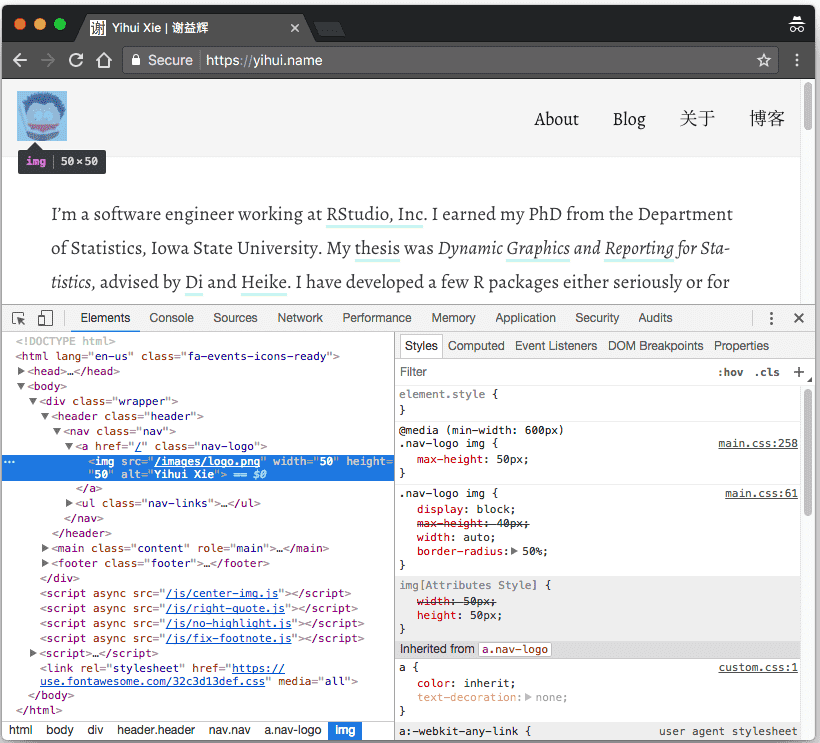
\includegraphics[width=1\linewidth]{images/chrome-devtools} 

}

\caption{Developer Tools in Google Chrome.}\label{fig:chrome-devtools}
\end{figure}

Typically you can also open the Developer Tools by right-clicking on a
certain element on the web page and selecting the menu item
\texttt{Inspect} (or \texttt{Inspect\ Element}). In Figure
\ref{fig:chrome-devtools}, I right-clicked on the profile image of my
website \url{https://yihui.name} and inspected it, and Chrome
highlighted its HTML source code
\texttt{\textless{}img\ src="..."\ ...\ /\textgreater{}} in the left
pane. You can also see the CSS styles associated with this \texttt{img}
element in the right pane. What is more, you can interactively change
the styles there if you know CSS, and see the (temporary) effects in
real time on the page! After you are satisfied with the new styles, you
can write the CSS code in files.

There are a lot of amazing features of Developer Tools, which make them
not only extremely useful for debugging and experimentation, but also
helpful for learning web development. These tools are indispensable to
me when I develop anything related to web pages. I learned a great deal
about CSS and JavaScript by playing with these tools.

\section{HTML}\label{html}

HTML\index{HTML} stands for Hyper Text Markup Language, and it is the
language behind most web pages you see. You can use the menu
\texttt{View\ -\textgreater{}\ View\ Source} or the context menu
\texttt{View\ Page\ Source} to see the full HTML source of a web page in
your browser. All elements on a page are represented by HTML tags. For
example, the tag \texttt{\textless{}p\textgreater{}} represents
paragraphs, and \texttt{\textless{}img\textgreater{}} represents images.

The good thing about HTML is that the language has only a limited number
of tags, and the number is not very big (especially the number of
commonly used tags). This means there is hope that you can master this
language fully and quickly.

Most HTML tags appear in pairs, with an opening tag and a closing tag,
e.g., \texttt{\textless{}p\textgreater{}\textless{}/p\textgreater{}}.
You write the content between the opening and closing tags, e.g.,
\texttt{\textless{}p\textgreater{}This\ is\ a\ paragraph.\textless{}/p\textgreater{}}.
There are a few exceptions, such as the
\texttt{\textless{}img\textgreater{}} tag, which can be closed by a
slash \texttt{/} in the opening tag, e.g.,
\texttt{\textless{}img\ src="foo.png"\ /\textgreater{}}. You can specify
attributes of an element in the opening tag using the syntax
\texttt{name=value} (a few attributes do not require \texttt{value}).

HTML documents often have the filename extension \texttt{.html} (or
\texttt{.htm}). Below is an overall structure of an HTML document:

\begin{Shaded}
\begin{Highlighting}[]
\KeywordTok{<html>}

  \KeywordTok{<head>}
  \KeywordTok{</head>}
  
  \KeywordTok{<body>}
  \KeywordTok{</body>}

\KeywordTok{</html>}
\end{Highlighting}
\end{Shaded}

Basically an HTML document consists a \texttt{head} section and
\texttt{body} section. You can specify the metadata and include assets
like CSS files in the \texttt{head} section. Normally the \texttt{head}
section is not visible on a web page. It is the \texttt{body} section
that holds the content to be displayed to a reader. Below is a slightly
richer example document:

\begin{Shaded}
\begin{Highlighting}[]
\DataTypeTok{<!DOCTYPE }\NormalTok{html}\DataTypeTok{>}
\KeywordTok{<html>}

  \KeywordTok{<head>}
    \KeywordTok{<meta}\OtherTok{ charset=}\StringTok{"utf-8"} \KeywordTok{/>}
    
    \KeywordTok{<title>}\NormalTok{Your Page Title}\KeywordTok{</title>}
    
    \KeywordTok{<link}\OtherTok{ rel=}\StringTok{"stylesheet"}\OtherTok{ href=}\StringTok{"/css/style.css"} \KeywordTok{/>}
  \KeywordTok{</head>}
  
  \KeywordTok{<body>}
    \KeywordTok{<h1>}\NormalTok{A First-level Heading}\KeywordTok{</h1>}
    
    \KeywordTok{<p>}\NormalTok{A paragraph.}\KeywordTok{</p>}
    
    \KeywordTok{<img}\OtherTok{ src=}\StringTok{"/images/foo.png"}\OtherTok{ alt=}\StringTok{"A nice image"} \KeywordTok{/>}
    
    \KeywordTok{<ul>}
      \KeywordTok{<li>}\NormalTok{An item.}\KeywordTok{</li>}
      \KeywordTok{<li>}\NormalTok{Another item.}\KeywordTok{</li>}
      \KeywordTok{<li>}\NormalTok{Yet another item.}\KeywordTok{</li>}
    \KeywordTok{</ul>}
    
    \KeywordTok{<script}\OtherTok{ src=}\StringTok{"/js/bar.js"}\KeywordTok{></script>}
  \KeywordTok{</body>}

\KeywordTok{</html>}
\end{Highlighting}
\end{Shaded}

In the head, we declare the character encoding of this page to be UTF-8
via a \texttt{\textless{}meta\textgreater{}} tag, specify the title via
the \texttt{\textless{}title\textgreater{}} tag, and include a
stylesheet via a \texttt{\textless{}link\textgreater{}} tag.

The body contains a first-level section heading
\texttt{\textless{}h1\textgreater{}},\footnote{There are six possible
  levels from \texttt{h1}, \texttt{h2}, \ldots{}, to \texttt{h6}.} a
paragraph \texttt{\textless{}p\textgreater{}}, an image
\texttt{\textless{}img\textgreater{}}, an unordered list
\texttt{\textless{}ul\textgreater{}} with three list items
\texttt{\textless{}li\textgreater{}}, and includes a JavaScript file in
the end via \texttt{\textless{}script\textgreater{}}.

There are much better tutorials on HTML than this section, such as those
offered by MDN and w3schools.com, so we are not going to make this
section a full tutorial. Instead, we just want to provide a few tips on
HTML:

\begin{itemize}
\item
  You may validate your HTML code via this service:
  \url{https://validator.w3.org}. This validator will point out
  potential problems of your HTML code. It actually works for XML and
  SVG documents, too.
\item
  Among all HTML attributes, file paths (the \texttt{src} attribute of
  some tags like \texttt{\textless{}img\textgreater{}}) and links (the
  \texttt{href} attribute of the \texttt{\textless{}a\textgreater{}}
  tag) may be the most confusing to beginners. Paths and links can be
  relative or absolute, and may come with or without the protocol and
  domain. You have to understand what a link or path exactly points to.
  A full link is of the form
  \texttt{http://www.example.com/foo/bar.ext}, where \texttt{http}
  specifies the protocol (it can be other protocols like \texttt{https}
  or \texttt{ftp}), \texttt{www.example.com} is the domain, and
  \texttt{foo/bar.ext} is the file under the root directory of the
  website.

  \begin{itemize}
  \item
    If you refer to resources on the same website (the same protocol and
    domain), we recommend that you omit the protocol and domain names,
    so that the links will continue to work even if you change the
    protocol or domain. For example, a link
    \texttt{\textless{}a\ href="/hi/there.html"\textgreater{}} on a page
    \texttt{http://example.com/foo/} refers to
    \texttt{http://example.com/hi/there.html}. It does not matter if you
    change \texttt{http} to \texttt{https}, or \texttt{example.com} to
    \texttt{another-domain.com}.
  \item
    Within the same website, a link or path can be relative or absolute.
    The meaning of an absolute path does not change no matter where the
    current HTML file is placed, but the meaning of a relative path
    depends on the location of the current HTML file. Suppose you are
    currently viewing the page \texttt{example.com/hi/there.html}:

    \begin{itemize}
    \item
      A absolute path \texttt{/foo/bar.ext} always means
      \texttt{example.com/foo/bar.ext}. The leading slash means the root
      directory of the website.
    \item
      A relative path \texttt{../images/foo.png} means
      \texttt{example.com/images/foo.png} (\texttt{..} means to go one
      level up). However, if the HTML file \texttt{there.html} is moved
      to \texttt{example.com/hey/again/there.html}, this path in
      \texttt{there.html} will refer to
      \texttt{example.com/hey/images/foo.png}.
    \item
      When deciding whether to use relative or absolute paths, here is
      the rule of thumb: if you will not move the resources referred or
      linked to from one subpath to another (e.g., from
      \texttt{example.com/foo/} to \texttt{example.com/bar/}), but only
      move the HTML pages that use these resources, use absolute paths;
      if you want to change the subpath of the URL of your website, but
      the relative locations of HTML files and the resources they use do
      not change, you may use relative links (e.g., you can move the
      whole website from \texttt{example.com/} to
      \texttt{example.com/foo/}).
    \item
      If the above concepts sound too complicated, a better way is to
      either think ahead carefully about the structure of your website
      and avoid moving files, or use rules of redirects if supported
      (such as 301 or 302 redirects).
    \end{itemize}
  \item
    If you link to a different website or web page, you have to include
    the domain in the link, but it may not be necessary to include the
    protocol, e.g., \texttt{//test.example.com/foo.css} is a valid path.
    The actual protocol of this path matches the protocol of the current
    page, e.g., if the current page is \texttt{https://example.com/},
    this link means \texttt{https://test.example.com/foo.css}. It may be
    beneficial to omit the protocol because HTTP resources cannot be
    embedded on pages served through HTTPS (for security reasons), e.g.,
    an image at \texttt{http://example.com/foo.png} cannot be embedded
    on a page \texttt{https://example.com/hi.html} via
    \texttt{\textless{}img\ src="http://example.com/foo.png"\ /\textgreater{}},
    but
    \texttt{\textless{}img\ src="//example.com/foo.png"\ /\textgreater{}}
    will work if the image can be accessed via HTTPS, i.e.,
    \texttt{https://example.com/foo.png}. The main drawback of not
    including the protocol is that such links and paths do not work if
    you open the HTML file locally without using a web server, e.g.,
    only double-click the HTML file in your file browser and show it in
    the browser.\footnote{That is because without a web server, an HTML
      file is viewed via the protocol \texttt{file}. For example, you
      may see a URL of the form \texttt{file://path/to/the/file.html} in
      the address bar of your browser. The path
      \texttt{//example.com/foo.png} will be interpreted as
      \texttt{file://example.com/foo.png}, which is unlikely to exist as
      a local file on your computer.}
  \item
    A very common mistake that people make is a link without the leading
    double slashes before the domain. You may think
    \texttt{www.example.com} is a valid link. It is not! At least it
    does not link to the website that you intend to link to. It works
    when you type it in the address bar of your browser because your
    browser will normally autocomplete it to
    \texttt{http://www.example.com}. However, if you write a link
    \texttt{\textless{}a\ href="www.example.com"\textgreater{}See\ this\ link\textless{}/a\textgreater{}},
    you will be in trouble. The browser will interpret this as a
    relative link, and it is relative to the URL of the current web
    page, e.g., if you are currently viewing
    \texttt{http://yihui.name/cn/}, the link \texttt{www.example.com}
    actually means \texttt{http://yihui.name/cn/www.example.com}! Now
    you should know the Markdown text
    \texttt{{[}Link{]}(www.example.com)} is typically a mistake, unless
    you really mean to link to a subdirectory of the current page or a
    file with literally the name \texttt{www.example.com}.
  \end{itemize}
\end{itemize}

\section{CSS}\label{css}

The Cascading Stylesheets\index{CSS} (CSS) language is used to describe
the look and formatting of documents written in HTML. CSS is responsible
for the visual style of your site. CSS is a lot of fun to play with, but
it can also easily steal your time.

In the Hugo framework
(\url{https://gohugo.io/tutorials/creating-a-new-theme/}), CSS is one of
the major ``non-content'' files that shapes the look and feel of your
site (the others are images, JavaScript, and Hugo templates). What does
the \href{https://en.wikipedia.org/wiki/Look_and_feel}{``look and
feel''} of a site mean? ``Look'' generally refers to static style
components including, but not limited to

\begin{itemize}
\tightlist
\item
  color palettes,
\item
  images,
\item
  layouts/margins, and
\item
  fonts.
\end{itemize}

whereas ``feel'' relates to dynamic components that the user interacts
with like

\begin{itemize}
\tightlist
\item
  dropdown menus,
\item
  buttons, and
\item
  forms.
\end{itemize}

There are 3 ways to define styles. The first is in line with HTML. For
example, this code

\begin{Shaded}
\begin{Highlighting}[]
\KeywordTok{<p>}\NormalTok{Marco! }\KeywordTok{<em>}\NormalTok{Polo!}\KeywordTok{</em></p>} 
\end{Highlighting}
\end{Shaded}

would produce text that looks like this: Marco! \emph{Polo!}

However, this method is generally not preferred for
\href{https://stackoverflow.com/q/12013532/559676}{numerous reasons.}

A second way is to internally define the CSS by placing a style section
in your HTML:

\begin{Shaded}
\begin{Highlighting}[]
\KeywordTok{<html>}
\KeywordTok{<style>} 
\FloatTok{#favorite} \KeywordTok{\{}
    \KeywordTok{font-style:} \DataTypeTok{italic}\KeywordTok{;}
\KeywordTok{\}}
\KeywordTok{</style>}
\KeywordTok{<ul}\OtherTok{ id=}\StringTok{"tea-list"}\KeywordTok{>}
  \KeywordTok{<li>}\NormalTok{Earl Grey}\KeywordTok{</li>}
  \KeywordTok{<li>}\NormalTok{Darjeeling}\KeywordTok{</li>}
  \KeywordTok{<li>}\NormalTok{Oolong}\KeywordTok{</li>}
  \KeywordTok{<li>}\NormalTok{Chamomile}\KeywordTok{</li>}
  \KeywordTok{<li}\OtherTok{ id=}\StringTok{"favorite"}\KeywordTok{>}\NormalTok{Chai}\KeywordTok{</li>}
\KeywordTok{</ul>}
\KeywordTok{</html>}
\end{Highlighting}
\end{Shaded}

In this example, only the last tea listed, \emph{Chai}, is italicized.

The third method is the most popular because it is more flexible and the
least repetitive. In this method, you define the CSS in an external file
that is then referenced as a link in your HTML:

\begin{Shaded}
\begin{Highlighting}[]
\KeywordTok{<html>}
    \KeywordTok{<link}\OtherTok{ rel=}\StringTok{"stylesheet"}\OtherTok{ href=}\StringTok{"/css/style.css"} \KeywordTok{/>}
\KeywordTok{</html>}
\end{Highlighting}
\end{Shaded}

What goes inside the linked CSS document is essentially a list of rules
(the same list could appear internally between the style tags, if you
are using the second method). Each rule must include both a selector or
group of selectors, and a declarations block within curly braces that
contains one or more \texttt{property:\ value;} pairs. Here is the
\href{https://developer.mozilla.org/en-US/docs/Web/CSS/Reference}{general
structure for a rule}:

\begin{Shaded}
\begin{Highlighting}[]
\CommentTok{/* CSS pseudo-code */}
\NormalTok{selectorlist }\KeywordTok{\{}
    \KeywordTok{property:}\NormalTok{ value}\KeywordTok{;}
    \CommentTok{/* more property: value; pairs*/}
\KeywordTok{\}}
\end{Highlighting}
\end{Shaded}

\href{https://developer.mozilla.org/en-US/docs/Web/CSS/Reference\#Selectors}{Selectors}
can be based on HTML element types or attributes, such as \texttt{id} or
\texttt{class} (and combinations of these attributes):

\begin{Shaded}
\begin{Highlighting}[]
\CommentTok{/* by element type */}
\NormalTok{li }\KeywordTok{\{} 
    \KeywordTok{color:} \DataTypeTok{yellow}\KeywordTok{;} \CommentTok{/* all <li> elements are yellow */}
\KeywordTok{\}}

\CommentTok{/* by ID with the # symbol */}
\FloatTok{#my-id} \KeywordTok{\{} 
    \KeywordTok{color:} \DataTypeTok{yellow}\KeywordTok{;} \CommentTok{/* elements with id = "my-id" are yellow */}
\KeywordTok{\}}

\CommentTok{/* by class with the . symbol */}
\FloatTok{.my-class} \KeywordTok{\{} 
    \KeywordTok{color:} \DataTypeTok{yellow}\KeywordTok{;} \CommentTok{/* elements with class = "my-class" are yellow  */}
\KeywordTok{\}}
\end{Highlighting}
\end{Shaded}

Because each HTML element may match several different selectors, the CSS
standard determines which set of rules has precedence for any given
element, and which properties to inherit. This is where the cascade
algorithm comes into play. For example, take a simple unordered list:

\begin{Shaded}
\begin{Highlighting}[]
\KeywordTok{<ul}\OtherTok{ id=}\StringTok{"tea-list"}\KeywordTok{>}
  \KeywordTok{<li>}\NormalTok{Earl Grey}\KeywordTok{</li>}
  \KeywordTok{<li>}\NormalTok{Darjeeling}\KeywordTok{</li>}
  \KeywordTok{<li>}\NormalTok{Oolong}\KeywordTok{</li>}
  \KeywordTok{<li>}\NormalTok{Chamomile}\KeywordTok{</li>}
  \KeywordTok{<li>}\NormalTok{Chai}\KeywordTok{</li>}
\KeywordTok{</ul>}
\end{Highlighting}
\end{Shaded}

Now, let's say we want to highlight our favorite teas again, so we'll
use a class attribute.

\begin{Shaded}
\begin{Highlighting}[]
\KeywordTok{<ul}\OtherTok{ id=}\StringTok{"tea-list"}\KeywordTok{>}
  \KeywordTok{<li>}\NormalTok{Earl Grey}\KeywordTok{</li>}
  \KeywordTok{<li}\OtherTok{ class=}\StringTok{"favorite"}\KeywordTok{>}\NormalTok{Darjeeling}\KeywordTok{</li>}
  \KeywordTok{<li>}\NormalTok{Oolong}\KeywordTok{</li>}
  \KeywordTok{<li>}\NormalTok{Chamomile}\KeywordTok{</li>}
  \KeywordTok{<li}\OtherTok{ class=}\StringTok{"favorite"}\KeywordTok{>}\NormalTok{Chai}\KeywordTok{</li>}
\KeywordTok{</ul>}
\end{Highlighting}
\end{Shaded}

We can use this class attribute as a selector in our CSS. Let's say we
want our favorite teas to be in bold and have a background color of
yellow, so our CSS would look like this:

\begin{Shaded}
\begin{Highlighting}[]
\FloatTok{.favorite} \KeywordTok{\{}
  \KeywordTok{font-weight:} \DataTypeTok{bold}\KeywordTok{;}
  \KeywordTok{background-color:} \DataTypeTok{yellow}\KeywordTok{;}
\KeywordTok{\}}
\end{Highlighting}
\end{Shaded}

Now, if you want every list item to be italicized with a white
background, you can set up another rule:

\begin{Shaded}
\begin{Highlighting}[]
\NormalTok{li }\KeywordTok{\{} 
  \KeywordTok{font-style:} \DataTypeTok{italic}\KeywordTok{;}
  \KeywordTok{background-color:} \DataTypeTok{white}\KeywordTok{;}
\KeywordTok{\}}
\end{Highlighting}
\end{Shaded}

If you play with this code (which you can do easily using sites like
\url{http://jsbin.com}, \url{https://jsfiddle.net}, or
\url{https://codepen.io/pen/}), you'll see that the two favorite teas
are still highlighted in yellow. This is because the CSS rule about
\texttt{.favorite} as a class is more specific than the rule about
\texttt{li} type elements. To override the \texttt{.favorite} rule, you
need to be as specific as you can be when choosing your group of
selectors:

\begin{Shaded}
\begin{Highlighting}[]
\NormalTok{ul}\FloatTok{#tea-list}\NormalTok{ li}\FloatTok{.favorite} \KeywordTok{\{}
  \KeywordTok{background-color:} \DataTypeTok{white}\KeywordTok{;}
\KeywordTok{\}}
\end{Highlighting}
\end{Shaded}

This example just scratches the surface of
\href{https://developer.mozilla.org/en-US/docs/Learn/CSS/Introduction_to_CSS/Cascade_and_inheritance}{cascade
and inheritance.}

For any Hugo theme that you install, you can find the CSS file in the
\texttt{themes/} folder. For example, the default lithium theme is
located in: \texttt{themes/hugo-lithium-theme/static/css/main.css}. Once
you are familiar with CSS, you can understand how each set of rules work
to shape the visual style of your website, and how to alter the rules.
For some themes (i.e., the
\href{https://github.com/gcushen/hugo-academic}{hugo-academic theme}),
you have the option of linking to a
\href{https://gist.github.com/gcushen/d5525a4506b9ccf83f2bce592a895495}{custom
CSS,} which you can use to further customize the visual style of your
site.

A few one-line examples illustrate how simple CSS rules can be used to
make dramatic changes:

\begin{itemize}
\item
  To make circular or rounded images, you may assign a class
  \texttt{img-circle} to images (e.g.,
  \texttt{\textless{}img\ class="img-circle"\ src="foo.png"\ /\textgreater{}})
  and define the CSS:

\begin{Shaded}
\begin{Highlighting}[]
\FloatTok{.img-circle} \KeywordTok{\{}
  \KeywordTok{border-radius:} \DataTypeTok{50%}\KeywordTok{;}
\KeywordTok{\}}
\end{Highlighting}
\end{Shaded}
\item
  To make striped tables, you can add background colors to odd or even
  rows of the table, e.g.,

\begin{Shaded}
\begin{Highlighting}[]
\NormalTok{tr}\DecValTok{:nth-child}\NormalTok{(even) }\KeywordTok{\{}
  \KeywordTok{background:} \DataTypeTok{#eee}\KeywordTok{;}
\KeywordTok{\}}
\end{Highlighting}
\end{Shaded}
\item
  You can append or prepend content to elements via pseudo-elements
  \texttt{::after} and \texttt{::before}. Here is an example of adding a
  period after section numbers:
  \url{https://github.com/rstudio/blogdown/issues/80}.
\end{itemize}

\section{JavaScript}\label{javascript}

It is way more challenging to briefly introduce
JavaScript\index{JavaScript} than HTML and CSS, since it is a
programming language. There are many books and tutorials about this
language. Anyway, we will try to scratch the surface for R users in this
section.

In a nutshell, JavaScript is a language that is typically used to
manipulate elements on a web page. An effective way to learn it is
through the JavaScript console in the Developer Tools of your web
browser (see Figure \ref{fig:chrome-devtools}), because you can
interactively type code in the console and execute it, which feels
similar to executing R code in the R console (e.g., in RStudio). You may
open any web page in your web browser (e.g., \url{https://yihui.name}),
then open the JavaScript console, and try the code below on any web
page:

\begin{Shaded}
\begin{Highlighting}[]
\VariableTok{document}\NormalTok{.}\VariableTok{body}\NormalTok{.}\VariableTok{style}\NormalTok{.}\AttributeTok{background} \OperatorTok{=} \StringTok{'orange'}\OperatorTok{;}
\end{Highlighting}
\end{Shaded}

It should change the background color of the page to orange, unless the
page has already defined background colors for certain elements.

To effectively use JavaScript, you have to learn both the basic syntax
of JavaScript and how to select elements on a page before you can
manipulate them. You may partially learn the former from the short
JavaScript snippet below:

\begin{Shaded}
\begin{Highlighting}[]
\KeywordTok{var}\NormalTok{ x }\OperatorTok{=} \DecValTok{1}\OperatorTok{;}  \CommentTok{// assignments}
\DecValTok{1} \OperatorTok{+} \DecValTok{2} \OperatorTok{-} \DecValTok{3} \OperatorTok{*} \DecValTok{4}\NormalTok{ / }\DecValTok{5}\OperatorTok{;}  \CommentTok{// arithmetic}

\ControlFlowTok{if}\NormalTok{ (x }\OperatorTok{<} \DecValTok{2}\NormalTok{) }\VariableTok{console}\NormalTok{.}\AttributeTok{log}\NormalTok{(x)}\OperatorTok{;}  \CommentTok{// "print" x}

\KeywordTok{var}\NormalTok{ y }\OperatorTok{=}\NormalTok{ [}\DecValTok{9}\OperatorTok{,} \DecValTok{1}\OperatorTok{,} \DecValTok{0}\OperatorTok{,} \DecValTok{2}\OperatorTok{,} \DecValTok{1}\OperatorTok{,} \DecValTok{4}\NormalTok{]}\OperatorTok{;}  \CommentTok{// array}

\CommentTok{// function}
\KeywordTok{var}\NormalTok{ sum }\OperatorTok{=} \KeywordTok{function}\NormalTok{(x) }\OperatorTok{\{}
  \KeywordTok{var}\NormalTok{ s }\OperatorTok{=} \DecValTok{0}\OperatorTok{;}
  \CommentTok{// a naive way to compute the sum}
  \ControlFlowTok{for}\NormalTok{ (}\KeywordTok{var}\NormalTok{ i}\OperatorTok{=}\DecValTok{0}\OperatorTok{;}\NormalTok{ i }\OperatorTok{<} \VariableTok{x}\NormalTok{.}\AttributeTok{length}\OperatorTok{;}\NormalTok{ i}\OperatorTok{++}\NormalTok{) }\OperatorTok{\{}
\NormalTok{    s }\OperatorTok{+=}\NormalTok{ x[i]}\OperatorTok{;}
  \OperatorTok{\}}
  \ControlFlowTok{return}\NormalTok{ s}\OperatorTok{;}
\OperatorTok{\};}

\AttributeTok{sum}\NormalTok{(y)}\OperatorTok{;}

\KeywordTok{var}\NormalTok{ y }\OperatorTok{=} \StringTok{"Hello World"}\OperatorTok{;}
\NormalTok{y }\OperatorTok{=} \VariableTok{y}\NormalTok{.}\AttributeTok{replace}\NormalTok{(}\StringTok{" "}\OperatorTok{,} \StringTok{", "}\NormalTok{)}\OperatorTok{;}  \CommentTok{// string manipulation}
\end{Highlighting}
\end{Shaded}

You may feel the syntax is similar to R to some degree. JavaScript is an
object-oriented language, and usually there are several methods that you
can apply to an object. The string manipulation above is a typical
example of the \texttt{Object.method()} syntax. To know the possible
methods on an object, you can type the object name in your JavaScript
console followed by a dot, and you should see all candidates.

R users have to be extremely cautious because JavaScript objects are
often mutable, meaning that an object could be modified anywhere. Below
is a quick example:

\begin{Shaded}
\begin{Highlighting}[]
\KeywordTok{var}\NormalTok{ x }\OperatorTok{=} \OperatorTok{\{}\StringTok{"a"}\OperatorTok{:} \DecValTok{1}\OperatorTok{,} \StringTok{"b"}\OperatorTok{:} \DecValTok{2}\OperatorTok{\};}  \CommentTok{// like a list in R}
\KeywordTok{var}\NormalTok{ f }\OperatorTok{=} \KeywordTok{function}\NormalTok{(z) }\OperatorTok{\{}
  \VariableTok{z}\NormalTok{.}\AttributeTok{a} \OperatorTok{=} \DecValTok{100}\OperatorTok{;}
\OperatorTok{\};}
\AttributeTok{f}\NormalTok{(x)}\OperatorTok{;}
\NormalTok{x}\OperatorTok{;}  \CommentTok{// modified! x.a is 100 now}
\end{Highlighting}
\end{Shaded}

There are many mature JavaScript libraries that can help you select and
manipulate elements on a page, and the most popular one may
be\index{jQuery} \href{https://jquery.com}{jQuery.} However, you should
know that sometimes you can probably do well enough without these
third-party libraries. There are some basic methods to select elements,
such as \texttt{document.getElementById()} and
\texttt{document.getElementsByClassName()}. For example, you can select
all paragraphs using
\texttt{document.querySelectorAll(\textquotesingle{}p\textquotesingle{})}.

Next we show a slightly advanced application, in which you will see
anonymous functions, selection of elements by HTML tag names, regular
expressions, and manipulation of HTML elements.

In Section \ref{how-to}, we mentioned how to enable
MathJax\index{MathJax} on a Hugo website. The easy part is to include
the script \texttt{MathJax.js} via a
\texttt{\textless{}script\textgreater{}} tag, and there are two hard
parts:

\begin{enumerate}
\def\labelenumi{\arabic{enumi}.}
\item
  How to protect the math content from the Markdown engine
  (Blackfriday), e.g., we need to make sure underscores in math
  expressions are not interpreted as
  \texttt{\textless{}em\textgreater{}\textless{}/em\textgreater{}}. This
  problem only exists in plain Markdown posts, and has been mentioned in
  Section \ref{output-format} without explaining the solution.
\item
  By default, MathJax does not recognize a pair of single dollar signs
  as the syntax for inline math expressions, but most users are perhaps
  more comfortable with the syntax \texttt{\$x\$} than
  \texttt{\textbackslash{}(x\textbackslash{})}.
\end{enumerate}

The easiest solution to the first problem may be adding backticks around
math expressions, e.g.,
\texttt{\textasciigrave{}\$x\_i\$\textasciigrave{}}, but the consequence
is that the math expression will be rendered in
\texttt{\textless{}code\textgreater{}\textless{}/code\textgreater{}},
and MathJax ignores \texttt{\textless{}code\textgreater{}} tags when
looking for math expressions on the page. We can force MathJax to search
for math expressions in \texttt{\textless{}code\textgreater{}}, but this
will still be problematic. For example, someone may want to display
inline R code \texttt{\textasciigrave{}list\$x\$y\textasciigrave{}}, and
\texttt{\$x\$} may be recognized as a math expression. MathJax ignores
\texttt{\textless{}code\textgreater{}} for good reasons. Even if you do
not have such expressions in \texttt{\textless{}code\textgreater{}}, you
may have some special CSS styles attached to
\texttt{\textless{}code\textgreater{}}, and these styles will be applied
to your math expressions, which can be undesired (e.g., a light gray
background).

To solve these problems, I have provided a solution in the JavaScript
code at \url{https://yihui.name/js/math-code.js}:

\begin{Shaded}
\begin{Highlighting}[]
\NormalTok{(}\KeywordTok{function}\NormalTok{() }\OperatorTok{\{}
  \KeywordTok{var}\NormalTok{ i}\OperatorTok{,}\NormalTok{ text}\OperatorTok{,}\NormalTok{ code}\OperatorTok{,}\NormalTok{ codes }\OperatorTok{=} \VariableTok{document}\NormalTok{.}\AttributeTok{getElementsByTagName}\NormalTok{(}\StringTok{'code'}\NormalTok{)}\OperatorTok{;}
  \ControlFlowTok{for}\NormalTok{ (i }\OperatorTok{=} \DecValTok{0}\OperatorTok{;}\NormalTok{ i }\OperatorTok{<} \VariableTok{codes}\NormalTok{.}\AttributeTok{length}\OperatorTok{;}\NormalTok{) }\OperatorTok{\{}
\NormalTok{    code }\OperatorTok{=}\NormalTok{ codes[i]}\OperatorTok{;}
    \ControlFlowTok{if}\NormalTok{ (}\VariableTok{code}\NormalTok{.}\VariableTok{parentNode}\NormalTok{.}\AttributeTok{tagName} \OperatorTok{!==} \StringTok{'PRE'} \OperatorTok{&&}
        \VariableTok{code}\NormalTok{.}\AttributeTok{childElementCount} \OperatorTok{===} \DecValTok{0}\NormalTok{) }\OperatorTok{\{}
\NormalTok{      text }\OperatorTok{=} \VariableTok{code}\NormalTok{.}\AttributeTok{textContent}\OperatorTok{;}
      \ControlFlowTok{if}\NormalTok{ (}\SpecialStringTok{/}\SpecialCharTok{^\textbackslash{}$[^$]}\SpecialStringTok{/}\NormalTok{.}\AttributeTok{test}\NormalTok{(text) }\OperatorTok{&&} \SpecialStringTok{/}\SpecialCharTok{[^$]\textbackslash{}$$}\SpecialStringTok{/}\NormalTok{.}\AttributeTok{test}\NormalTok{(text)) }\OperatorTok{\{}
\NormalTok{        text }\OperatorTok{=} \VariableTok{text}\NormalTok{.}\AttributeTok{replace}\NormalTok{(}\SpecialStringTok{/}\SpecialCharTok{^\textbackslash{}$}\SpecialStringTok{/}\OperatorTok{,} \StringTok{'}\SpecialCharTok{\textbackslash{}\textbackslash{}}\StringTok{('}\NormalTok{).}\AttributeTok{replace}\NormalTok{(}\SpecialStringTok{/}\SpecialCharTok{\textbackslash{}$$}\SpecialStringTok{/}\OperatorTok{,} \StringTok{'}\SpecialCharTok{\textbackslash{}\textbackslash{}}\StringTok{)'}\NormalTok{)}\OperatorTok{;}
        \VariableTok{code}\NormalTok{.}\AttributeTok{textContent} \OperatorTok{=}\NormalTok{ text}\OperatorTok{;}
      \OperatorTok{\}}
      \ControlFlowTok{if}\NormalTok{ (}\SpecialStringTok{/}\SpecialCharTok{^\textbackslash{}\textbackslash{}\textbackslash{}((}\SpecialStringTok{.}\SpecialCharTok{|\textbackslash{}s)+\textbackslash{}\textbackslash{}\textbackslash{})$}\SpecialStringTok{/}\NormalTok{.}\AttributeTok{test}\NormalTok{(text) }\OperatorTok{||}
          \SpecialStringTok{/}\SpecialCharTok{^\textbackslash{}\textbackslash{}\textbackslash{}[(}\SpecialStringTok{.}\SpecialCharTok{|\textbackslash{}s)+\textbackslash{}\textbackslash{}\textbackslash{}]$}\SpecialStringTok{/}\NormalTok{.}\AttributeTok{test}\NormalTok{(text) }\OperatorTok{||}
          \SpecialStringTok{/}\SpecialCharTok{^\textbackslash{}$(}\SpecialStringTok{.}\SpecialCharTok{|\textbackslash{}s)+\textbackslash{}$$}\SpecialStringTok{/}\NormalTok{.}\AttributeTok{test}\NormalTok{(text) }\OperatorTok{||}
          \SpecialStringTok{/}\SpecialCharTok{^\textbackslash{}\textbackslash{}}\SpecialStringTok{begin}\SpecialCharTok{\textbackslash{}\{([^\}]+)\textbackslash{}\}(}\SpecialStringTok{.}\SpecialCharTok{|\textbackslash{}s)+\textbackslash{}\textbackslash{}}\SpecialStringTok{end}\SpecialCharTok{\textbackslash{}\{[^\}]+\textbackslash{}\}$}\SpecialStringTok{/}\NormalTok{.}\AttributeTok{test}\NormalTok{(text)) }\OperatorTok{\{}
        \VariableTok{code}\NormalTok{.}\AttributeTok{outerHTML} \OperatorTok{=} \VariableTok{code}\NormalTok{.}\AttributeTok{innerHTML}\OperatorTok{;}  \CommentTok{// remove <code></code>}
        \ControlFlowTok{continue}\OperatorTok{;}
      \OperatorTok{\}}
    \OperatorTok{\}}
\NormalTok{    i}\OperatorTok{++;}
  \OperatorTok{\}}
\OperatorTok{\}}\NormalTok{)()}\OperatorTok{;}
\end{Highlighting}
\end{Shaded}

It is not a perfect solution, but it should be very rare that you run
into problems. This solution identifies possible math expressions in
\texttt{\textless{}code\textgreater{}}, and strips the
\texttt{\textless{}code\textgreater{}} tag, e.g., replaces
\texttt{\textless{}code\textgreater{}\$x\$\textless{}/code\textgreater{}}
with \texttt{\textbackslash{}(x\textbackslash{})}. After this script is
executed, we load the MathJax script. This way, we do not need to force
MathJax to search for math expressions in
\texttt{\textless{}code\textgreater{}} tags, and your math expressions
will not inherit any styles from \texttt{\textless{}code\textgreater{}}.
The JavaScript code above is not too long, and should be
self-explanatory. The trickiest part is \texttt{i++}. I will leave it to
readers to figure out why the \texttt{for} loop is not the usual form
\texttt{for\ (i\ =\ 0;\ i\ \textless{}\ codes.length;\ i++)}. It took me
quite a few minutes to realize my mistake when I wrote the loop in the
usual form.

\section{Useful resources}\label{useful-resources}

\subsection{File optimization}\label{file-optimization}

Although\index{Optimization} static websites are fast in general, you
can certainly further optimize them. You may search for ``CSS and
JavaScript minifier,'' and these tools can compress your CSS and
JavaScript files, so that they can be loaded faster. Since there are a
lot of tools, I will not recommend any here.

You can also optimize images on your website. I frequently use a
command-line tool named
\href{http://optipng.sourceforge.net}{\texttt{optipng}} to optimize PNG
images. It is a lossless optimizer, meaning that it reduces the file
size of a PNG image without loss of quality. From my experience, it
works very well on PNG images generated from R, and can reduce the file
size by at least 30\% (sometimes even more than 50\%). Personally I also
use online tools like \url{http://optimizilla.com} to optimize PNG and
JPEG images. For GIF images, I often use
\url{https://ezgif.com/optimize} to reduce the file sizes if they are
too big.

Note that Netlify has provided the optimization features on the server
side for free at the moment, so you may just want to enable them there
instead of doing all the hard work by yourself.

\subsection{Helping people find your
site}\label{helping-people-find-your-site}

Once your site is up and running, you probably want people to find it.
SEO --- Search Engine Optimization --- is the art of making a website
easy for search engines like Google to understand. And, hopefully, if
the search engine knows what you are writing about, it will present
links to your site high in results when someone searches for topics you
cover.

Entire books have been written about SEO, not to mention the many
companies that are in the business of offering (paid) technical and
strategic advice to help get sites atop search-engine rankings. If you
are interested in finding out more, a good place to start is the Google
Search Engine Optimization Starter Guide
(\url{http://bit.ly/google-seo-starter}). Below are a few key points:

\begin{enumerate}
\def\labelenumi{\arabic{enumi}.}
\item
  The title that you select for each page and post is a very important
  signal to Google and other search engines telling them what that page
  is about.
\item
  Description tags are also critical to explain what a page is about. In
  HTML documents,
  \href{https://www.w3schools.com/tags/tag_meta.asp}{description tags}
  are one way to provide metadata about the page. Using
  \textbf{blogdown}, the description may end up as text under the page
  title in a search-engine result. If your page's YAML does not include
  a description, you can add one like
  \texttt{description:\ "A\ brief\ description\ of\ this\ page."}; the
  HTML source of the rendered page would have a
  \texttt{\textless{}meta\textgreater{}} tag in
  \texttt{\textless{}head\textgreater{}} like
  \texttt{\textless{}meta\ name="description"\ content="A\ brief\ description\ of\ this\ page."\textgreater{}}.
  Not all themes support adding the description to your HTML page
  (although they should!)
\item
  URL structure also matters. You want your post's slug to have
  informative keywords, which gives another signal of what the page is
  about. Have a post with interesting things to do in San Francisco?
  \texttt{san-francisco-events-calendar} might be a better slug than
  \texttt{my-guide-to-fun-things-to-do}.
\end{enumerate}

\chapter{Domain Name}\label{domain-name}

While you can use the free subdomain names\index{Domain Name} like those
provided by GitHub or Netlify, it may be a better idea to own a domain
name of your own. The cost of an apex domain is minimal (typically the
yearly cost is about US\$10), and you will enter a much richer world
after you purchase a domain name. For example, you are free to point
your domain to any web servers, you can create as many subdomain names
as you want, and you can even set up your own email accounts using the
domain or subdomains. In this appendix, we will explain some basic
concepts of domain names, and mention a few (free) services to help you
configure your domain name.

Before we dive into the details, we want to outline the big picture of
how a URL works in your web browser. Suppose you typed or clicked a link
\texttt{http://www.example.com/foo/index.html} in your web browser. What
happens behind the scenes before you see the actual web page?

First, the domain name has to be resolved through the nameservers
associated with it. A nameserver knows the DNS (Domain Name System)
records of a domain. Typically it will look up the ``A records'' to
point the domain to the IP address of a web server. There are several
other types of DNS records, and we will explain them later. Once the web
server is reached, the server will look for the file
\texttt{foo/index.html} under a directory associated with the domain
name, and return its content in the response. That is basically how you
can see a web page.

\section{Registration}\label{registration}

You can purchase a domain name from many domain name registrars. To stay
neutral, we are not going to make recommendations here. You can use your
search engine to find a registrar by yourself, or ask your friends for
recommendations. However, we would like to remind you of a few things
that you should pay attention to when looking for a domain name
registrar:

\begin{itemize}
\item
  You should have the freedom to transfer your domain from the current
  registrar to other registrars, i.e., they should not lock you in their
  system. To transfer a domain name, you should be given a code known as
  the ``Transfer Auth Code'' or ``Auth Code'' or ``Transfer Key'' or
  something like that.
\item
  You should be able to customize the nameservers (see Section
  \ref{nameservers}) of your domain. By default, each registrar will
  assign their own nameservers to you, and these nameservers typically
  work very well. However, there are some special nameservers that
  provide services more than just DNS records, and you may be interested
  in using them.
\item
  Other people can freely look up your personal information, such as
  your email or postal address, after you register a domain and submit
  this information to the registrar. This is called the ``WHOIS
  Lookup.'' You may want to protect your privacy, but your registrar may
  require an extra payment.
\end{itemize}

\section{Nameservers}\label{nameservers}

The main reason why we need nameservers\index{Nameservers} is that we
want to use domains instead of IP addresses, although a domain is not
strictly necessary for you to be able to access a website. You could use
the IP address if you have your own server with a public IP, but there
are many problems with this approach. For example, IP addresses are
limited (in particular IPv4), not easy to memorize, and you can only
host one website per IP address (without using other ports).

A nameserver is an engine that directs the DNS records of your domain.
The most common DNS record is the A record, which maps a domain to an IP
address, so that the hosting server can be found via its IP address when
a website is accessed through a domain. We will introduce two more types
of DNS records in Section \ref{dns-records}: CNAME and MX records.

In most cases, the default nameservers provided by your domain registrar
should suffice, but there is a special technology missing in most
nameservers: CNAME flattening. You only need this technology if you want
to set a CNAME record for your apex domain. The only use case to my
knowledge is when you host your website via Netlify, but want to use the
apex domain instead of the \texttt{www} subdomain, e.g., you want to use
\texttt{example.com} instead of \texttt{www.example.com}. To make use of
this technology, you could consider
\href{https://www.cloudflare.com}{Cloudflare,} which provides this DNS
feature for free. Basically, all you need to do is to point the
nameservers of your domain to the nameservers provided by Cloudflare (of
the form \texttt{*.ns.cloudflare.com}).

\section{DNS records}\label{dns-records}

There are many types of DNS\index{DNS Records} records, and you may see
a full list on
\href{https://en.wikipedia.org/wiki/List_of_DNS_record_types}{Wikipedia.}
The most commonly used types may be A, CNAME, and MX records. Figure
\ref{fig:cloudflare-dns} shows a subset of DNS records of my domain
\texttt{yihui.name} on Cloudflare, which may give you an idea of what
DNS records look like. You may query DNS records using command-line
tools such as
\href{https://en.wikipedia.org/wiki/Dig_(command)}{\texttt{dig}} or an
app provided by Google: \url{https://toolbox.googleapps.com/apps/dig/}.

\begin{figure}

{\centering 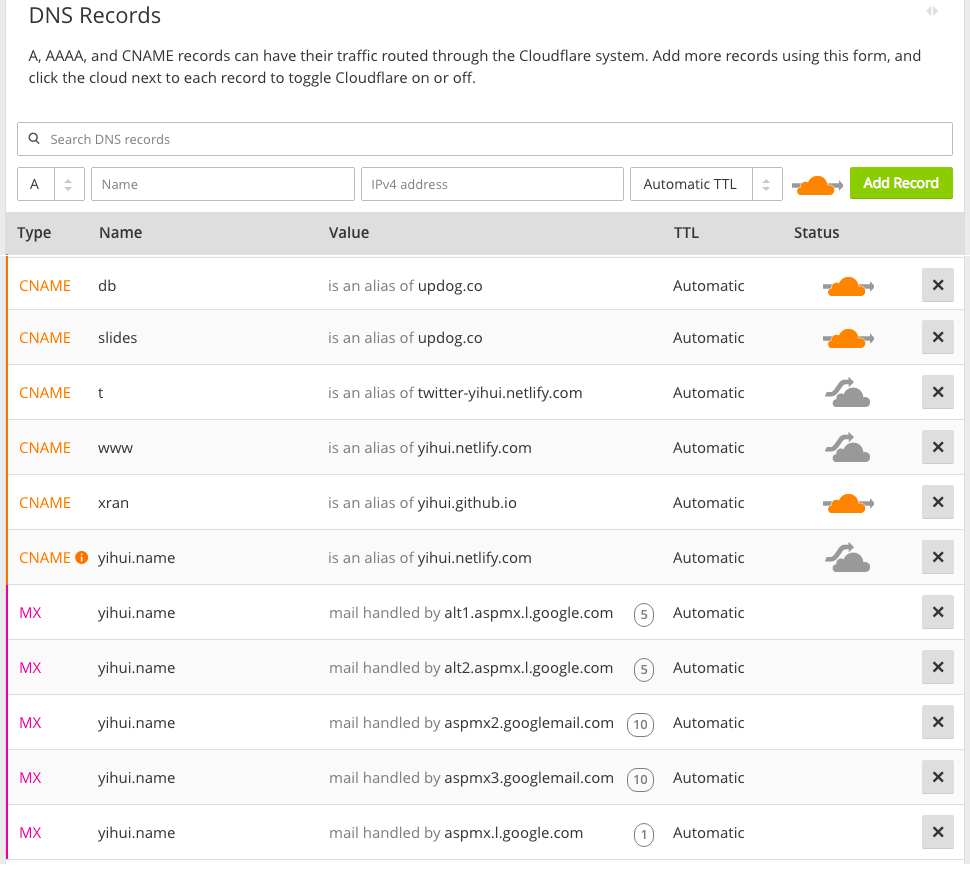
\includegraphics[width=1\linewidth]{images/cloudflare-dns} 

}

\caption{Some DNS records of the domain yihui.name on Cloudflare.}\label{fig:cloudflare-dns}
\end{figure}

An apex domain can have any number of subdomains. You can set DNS
records for the apex domain and any subdomains. You can see from Figure
\ref{fig:cloudflare-dns} that I have several subdomains, e.g.,
\texttt{slides.yihui.name} and \texttt{xran.yihui.name}.

As we have mentioned, an A record points a domain or subdomain to an IP
address of the host server. I did not use any A records for my domains
since all services I use, such as Updog, GitHub Pages, and Netlify,
support CNAME records well. A CNAME\index{CNAME Record} record is an
alias, pointing one domain to another domain. The advantage of using
CNAME over A is that you do not have to tie a domain to a fixed IP
address. For example, the CNAME record for \texttt{t.yihui.name} is
\texttt{twitter-yihui.netlify.com}. The latter domain is provided by
Netlify, and I do not need to know where they actually host the website.
They are free to move the host of \texttt{twitter-yihui.netlify.com},
and I will not need to update my DNS record. Every time someone visits
the website \texttt{t.yihui.name}, the web browser will route the
traffic to the domain set in the CNAME record. Note that this is
different from redirection, i.e., the URL \texttt{t.yihui.name} will not
be explicitly redirected to \texttt{twitter-yihui.netlify.com} (you
still see the former in the address bar of your browser).

Normally, you can set any DNS records for the apex domain except CNAME,
but I set a CNAME record for my apex domain \texttt{yihui.name}, and
that is because Cloudflare supports CNAME flattening. For more
information on this topic, you may read the post
\href{https://www.netlify.com/blog/2017/02/28/to-www-or-not-www/}{``To
WWW or not WWW,''} by Netlify. Personally, I prefer not using the
subdomain \texttt{www.yihui.name} to keep my URLs short, so I set a
CNAME record for both the apex domain \texttt{yihui.name} and the
\texttt{www} subdomain, and Netlify will automatically redirect the
\texttt{www} subdomain to the apex domain. That said, if you are a
beginner, it may be a little easier to configure and use the
\texttt{www} subdomain, as suggested by Netlify. Note \texttt{www} is a
conventional subdomain that sounds like an apex domain, but really is
not; you can follow this convention or not as you wish.

For email services, I was an early enough
\href{https://en.wikipedia.org/wiki/Netizen}{``netizen'',} and when I
registered my domain name, Google was still offering free email services
to custom domain owners. That is how I can have a custom mailbox
\texttt{xie@yihui.name}. Now you will have to pay for
\href{https://gsuite.google.com}{G Suite.} In Figure
\ref{fig:cloudflare-dns} you can see I have set some MX (stands for
``mail exchange'') records that point to some Google mail servers. Of
course, Google is not the only possible choice when it comes to custom
mailboxes. \href{https://www.migadu.com}{Migadu} claims to be the ``most
affordable email hosting.'' You may try its free plan and see if you
like it. Unless you are going to use your custom mailbox extensively and
for professional purposes, the free plan may suffice. In fact, you may
create an alias address on Migadu to forward emails to your other email
accounts (such as Gmail) if you do not care about an actual custom
mailbox. Migadu has provided detailed instructions on how to set the MX
records for your domain.

\chapter{Advanced Topics}\label{advanced-topics}

In this appendix, we talk about a few advanced topics that may be of
interest to developers and advanced users.

\section{More global options}\label{more-global-options}

There are a few more advanced global options\index{Global Options} in
addition to those introduced in Section \ref{global-options}, and they
are listed in Table \ref{tab:global-options2}.

\begin{table}

\caption{\label{tab:global-options2}A few more advanced global options.}
\centering
\begin{tabular}[t]{lll}
\toprule
Option name & Default & Meaning\\
\midrule
blogdown.hugo.dir &  & The directory of the Hugo executable\\
blogdown.method & html & The building method for R Markdown\\
blogdown.publishDir &  & The publish dir for local preview\\
blogdown.widgetsID & TRUE & Incremental IDs for HTML widgets?\\
\bottomrule
\end{tabular}
\end{table}

If you want to install Hugo to a custom path, you can set the global
option \texttt{blogdown.hugo.dir} to a directory to store the Hugo
executable before you call \texttt{install\_hugo()}, e.g.,
\texttt{options(blogdown.hugo.dir\ =\ \textquotesingle{}\textasciitilde{}/Downloads/hugo\_0.20.1/\textquotesingle{})}.
This may be useful for you to use a specific version of Hugo for a
specific website,\footnote{You can set this option per project. See
  Section \ref{global-options} for details.} or store a copy of Hugo on
a USB Flash drive along with your website.

The option \texttt{blogdown.method} is explained in Section
\ref{methods}.

When your website project is under version control in the RStudio IDE,
continuously previewing the site can be slow, if it contains hundreds of
files or more. The default publish directory is \texttt{public/} under
the project root directory, and whenever you make a change in the source
that triggers a rebuild, RStudio will be busy tracking file changes in
the \texttt{public/} directory. The delay before you see the website in
the RStudio Viewer can be 10 seconds or even longer. That is why we
provide the option \texttt{blogdown.publishDir}. You may set a temporary
publish directory to generate the website, and this directory should not
be under the same RStudio project, e.g.,
\texttt{options(blogdown.publishDir\ =\ \textquotesingle{}../public\_site\textquotesingle{})},
which means the website will be generated to the directory
\texttt{public\_site/} under the parent directory of the current
project.

The option \texttt{blogdown.widgetsID} is only relevant if your website
source is under version control and you have HTML widgets on the
website. If this option is \texttt{TRUE} (default), the random IDs of
HTML widgets will be changed to incremental IDs in the HTML output, so
these IDs are unlikely to change every time you recompile your website;
otherwise, every time you will get different random IDs.

\section{LiveReload}\label{livereload}

As we briefly mentioned\index{LiveReload} in Section
\ref{a-quick-example}, you can use \texttt{blogdown::serve\_site()} to
preview a website, and the web page will be automatically rebuilt and
reloaded in your web browser when the source file is modified and saved.
This is called ``LiveReload.''

We have provided two approaches to LiveReload. The default approach is
through \texttt{servr::httw()}, which will continuously watch the
website directory for file changes, and rebuild the site when changes
are detected. This approach has a few drawbacks:

\begin{enumerate}
\def\labelenumi{\arabic{enumi}.}
\item
  It is relatively slow because the website is fully regenerated every
  time. This may not be a real problem for Hugo, because Hugo is often
  fast enough: it takes about a millisecond to generate one page, so a
  website with a thousand pages may only take about one second to be
  fully regenerated.
\item
  The daemonized server (see Section \ref{global-options}) may not work.
\end{enumerate}

If you are not concerned about the above issues, we recommend that you
use the default approach, otherwise you can set the global option
\texttt{options(blogdown.generator.server\ =\ TRUE)} to use an
alternative approach to LiveReload, which is based on the native support
for LiveReload from the static site generator. At the moment, this has
only been tested against Hugo-based websites. It does not work with
Jekyll and we were not successful with Hexo, either.

This alternative approach requires two additional R packages to be
installed: \textbf{processx} \citep{R-processx} and \textbf{later}
\citep{R-later}. You may use this approach when you primarily work on
plain Markdown posts instead of R Markdown posts, because it can be much
faster to preview Markdown posts using the web server of Hugo. The web
server can be stopped by \texttt{blogdown::stop\_server()}, and it will
always be stopped when the R session is ended, so you can restart your R
session if \texttt{stop\_server()} fails to stop the server for some
reason.

The web server is established via the command \texttt{hugo\ server} (see
\href{https://gohugo.io/commands/hugo_server/}{its documentation} for
details). You can pass command-line arguments via the global option
\texttt{blogdown.hugo.server}. The default value for this option is
\texttt{c(\textquotesingle{}-D\textquotesingle{},\ \textquotesingle{}-F\textquotesingle{})},
which means to render draft and future posts in the preview. We want to
highlight a special argument \texttt{-\/-navigateToChanged} in a recent
version of Hugo, which asks Hugo to automatically navigate to the
changed page. For example, you can set the options:

\begin{Shaded}
\begin{Highlighting}[]
\KeywordTok{options}\NormalTok{(}\DataTypeTok{blogdown.hugo.server =} \KeywordTok{c}\NormalTok{(}\StringTok{'-D'}\NormalTok{, }\StringTok{'-F'}\NormalTok{, }\StringTok{'--navigateToChanged'}\NormalTok{))}
\end{Highlighting}
\end{Shaded}

Then, when you edit a source file under \texttt{content/}, Hugo will
automatically show you the corresponding output page in the web browser.

Note that Hugo renders and serves the website from memory by default, so
no files will be generated to \texttt{public/}. If you need to publish
the \texttt{public/} folder manually, you will have to manually build
the website via \texttt{blogdown::hugo\_build()} or
\texttt{blogdown::build\_site()}.

\section{Building a website for local preview}\label{local-preview}

The function\index{blogdown::build\_site()}
\texttt{blogdown::build\_site()} has an argument \texttt{local} that
defaults to \texttt{FALSE}, which means building the website for
publishing instead of local previewing. The mode \texttt{local\ =\ TRUE}
is primarily for \texttt{blogdown::serve\_site()} to serve the website
locally. There are three major differences between
\texttt{local\ =\ FALSE} and \texttt{TRUE}. When
\texttt{local\ =\ TRUE}:

\begin{itemize}
\item
  The \texttt{baseurl} option in \texttt{config.toml} is temporarily
  overridden by \texttt{"/"} even if you have set it to a full URL like
  \texttt{"http://www.example.com/"}.\footnote{If your \texttt{baseurl}
    contains a subdirectory, it will be overridden by the subdirectory
    name. For example, for
    \texttt{baseurl\ =\ "http://www.example.com/project/"},
    \texttt{build\_site(local\ =\ TRUE)} will temporarily remove the
    domain name and only use the value \texttt{/project/}.} This is
  because when a website is to be previewed locally, links should refer
  to local files. For example, \texttt{/about/index.html} should be used
  instead of the full link
  \texttt{http://www.example.com/about/index.html}; the function
  \texttt{serve\_site()} knows that \texttt{/about/index.html} means the
  file under the \texttt{public/} directory, and can fetch it and
  display the content to you, otherwise your browser will take you to
  the website \texttt{http://www.example.com} instead of displaying a
  local file.
\item
  Draft and future posts are always rendered when
  \texttt{local\ =\ TRUE}, but not when \texttt{local\ =\ FALSE}. This
  is for you to preview draft and future posts locally. If you know the
  \href{https://gohugo.io/commands/hugo/}{Hugo command line,} it means
  the \texttt{hugo} command is called with the flags \texttt{-D\ -F}, or
  equivalently, \texttt{-\/-buildDrafts\ -\/-buildFuture}.
\item
  There is a caching mechanism to speed up building your website: an Rmd
  file will not be recompiled when its \texttt{*.html} output file is
  newer (in terms of file modification time). If you want to force
  \texttt{build\_site(local\ =\ TRUE)} to recompile the Rmd file even if
  it is older than the HTML output, you need to delete the HTML output,
  or edit the Rmd file so that its modification time will be newer. This
  caching mechanism does not apply to \texttt{local\ =\ FALSE}, i.e.,
  \texttt{build\_site(local\ =\ FALSE)} will always recompile all Rmd
  files, because when you want to publish a site, you may need to
  recompile everything to make sure the site is fully regenerated. If
  you have time-consuming code chunks in any Rmd files, you have to use
  either of these methods to save time:

  \begin{itemize}
  \item
    Turn on \textbf{knitr}'s caching for time-consuming code chunks,
    i.e., the chunk option \texttt{cache\ =\ TRUE}.
  \item
    Do not call \texttt{build\_site()}, but
    \texttt{blogdown::hugo\_build()}
    instead\index{blogdown::hugo\_build()}. The latter does not compile
    any Rmd files, but simply runs the \texttt{hugo} command to build
    the site. Please use this method only if you are sure that your Rmd
    files do not need to be recompiled.
  \end{itemize}
\end{itemize}

You do not need to worry about these details if your website is
automatically generated from source via a service like Netlify, which
will make use of \texttt{baseurl} and not use \texttt{-D\ -F} by
default. If you manually publish the \texttt{public/} folder, you need
to be more careful:

\begin{itemize}
\item
  If your website does not work without the full \texttt{baseurl}, or
  you do not want the draft or future posts to be published, you should
  not publish the \texttt{public/} directory generated by
  \texttt{serve\_site()}. Always run \texttt{blogdown::build\_site()} or
  \texttt{blogdown::hugo\_build()} before you upload this directory to a
  web server.
\item
  If your drafts and future posts contain (time-)sensitive information,
  you are strongly recommended to delete the \texttt{/public/} directory
  before you rebuild the site for publishing every time, because Hugo
  never deletes it, and your sensitive information may be rendered by a
  certain \texttt{build\_site(local\ =\ TRUE)} call last time and left
  in the directory. If the website is really important, and you need to
  make sure you absolutely will not screw up anything every time you
  publish it, put the \texttt{/public/} directory under version control,
  so you have a chance to see which files were changed before you
  publish the new site.
\end{itemize}

\section{Functions in the blogdown package}\label{functions}

There are about 20 exported functions\index{Functions} in the
\textbf{blogdown} package, and many more non-exported functions.
Exported functions are documented and you can use them after
\texttt{library(blogdown)} (or via \texttt{blogdown::}). Non-exported
functions are not documented, but you can access them via
\texttt{blogdown:::} (the triple-colon syntax). This package is not very
complicated, and consists of only about 1800 lines of R code (the number
is given by the word-counting command \texttt{wc}):

You may take a look at the source code
(\url{https://github.com/rstudio/blogdown}) if you want to know more
about a non-exported function. In this section, we selectively list some
exported and non-exported functions in the package for your reference.

\subsection{Exported functions}\label{exported-functions}

Installation: You can install Hugo with \texttt{install\_hugo()}, update
Hugo with \texttt{update\_hugo()}, and install a Hugo theme with
\texttt{install\_theme()}.

Wrappers of Hugo commands: \texttt{hugo\_cmd()} is a general wrapper of
\texttt{system2(\textquotesingle{}hugo\textquotesingle{},\ ...)}, and
all later functions execute specific Hugo commands based on this general
wrapper function; \texttt{hugo\_version()} executes the command
\texttt{hugo\ version} (i.e.,
\texttt{system2(\textquotesingle{}hugo\textquotesingle{},\ \textquotesingle{}version\textquotesingle{})}
in R); \texttt{hugo\_build()} executes \texttt{hugo} with optional
parameters; \texttt{new\_site()} executes \texttt{hugo\ new\ site};
\texttt{new\_content()} executes \texttt{hugo\ new} to create a new
content file, and \texttt{new\_post()} is a wrapper based on
\texttt{new\_content()} to create a new blog post with appropriate YAML
metadata and filename; \texttt{hugo\_convert()} executes
\texttt{hugo\ convert}; \texttt{hugo\_server()} executes
\texttt{hugo\ server}.

Output format: \texttt{html\_page()} is the only R Markdown output
format function in the package. It inherits from
\texttt{bookdown::html\_document2()}, which in turn inherits from
\texttt{rmarkdown::html\_document()}. You need to read the documentation
of these two functions to know the possible arguments. Section
\ref{output-format} has more detailed information about it.

Helper functions: \texttt{shortcode()} is a helper function to write a
Hugo shortcode \texttt{\{\{\%\ \%\}\}} in an Rmd post;
\texttt{shortcode\_html()} writes out
\texttt{\{\{\textless{}\ \textgreater{}\}\}}.

Serving a site: \texttt{serve\_site()} starts a local web server to
build and preview a site continuously; you can stop the server via
\texttt{stop\_server()}, or restart your R session.

Dealing with YAML metadata: \texttt{find\_yaml()} can be used to find
content files that contain a specified YAML field with specified values;
\texttt{find\_tags()} and \texttt{find\_categories()} are wrapper
functions based on \texttt{find\_yaml()} to match specific tags and
categories in content files, respectively; \texttt{count\_yaml()} can be
used to calculate the frequencies of specified fields.

\subsection{Non-exported functions}\label{non-exported-functions}

Some functions are not exported in this package because average users
are unlikely to use them directly, and we list a subset of them below:

\begin{itemize}
\item
  You can find the path to the Hugo executable via
  \texttt{blogdown:::find\_hugo()}. If the executable can be found via
  the \texttt{PATH} environment variable, it just returns
  \texttt{\textquotesingle{}hugo\textquotesingle{}}.
\item
  The helper function \texttt{modify\_yaml()} can be used to modify the
  YAML metadata of a file. It has a \texttt{...} argument that takes
  arbitrary YAML fields, e.g.,
  \texttt{blogdown:::modify\_yaml(\textquotesingle{}foo.md\textquotesingle{},\ author\ =\ \textquotesingle{}Frida\ Gomam\textquotesingle{},\ date\ =\ \textquotesingle{}2015-07-23\textquotesingle{})}
  will change the \texttt{author} field in the file \texttt{foo.md} to
  \texttt{Frida\ Gomam}, and \texttt{date} to \texttt{2015-07-23}. We
  have shown the advanced usage of this function in Section
  \ref{from-jekyll}.
\item
  We have also mentioned a series of functions to clean up Markdown
  posts in Section \ref{from-jekyll}. They include
  \texttt{process\_file()}, \texttt{remove\_extra\_empty\_lines()},
  \texttt{process\_bare\_urls()}, \texttt{normalize\_chars()},
  \texttt{remove\_highlight\_tags()}, and \texttt{fix\_img\_tags()}.
\item
  In Section \ref{local-preview}, we mentioned a caching mechanism based
  on the file modification time. It is implemented in
  \texttt{blogdown:::require\_rebuild()}, which takes two arguments of
  filenames. The first file is the output file, and the second is the
  source file. When the source file is older than the output file, or
  the output file does not exist or is empty, this function returns
  \texttt{TRUE}.
\item
  The function \texttt{blogdown:::Rscript()} is a wrapper function to
  execute the command \texttt{Rscript}, which basically means to execute
  an R script in a new R session. We mentioned this function in Chapter
  \ref{other-generators}.
\end{itemize}

\section{Paths of figures and other dependencies}\label{dep-path}

One of the most challenging tasks in developing the \textbf{blogdown}
package is to properly handle dependency files\index{Dependency Files}
of web pages. If all pages of a website were plain text without
dependencies like images or JavaScript libraries, it would be much
easier for me to develop the \textbf{blogdown} package.

After \textbf{blogdown} compiles each Rmd document to HTML, it will try
to detect the dependencies (if there are any) from the HTML source and
copy them to the \texttt{static/} folder, so that Hugo will copy them to
\texttt{public/} later. The detection depends on the paths of
dependencies. By default, all dependencies, like R plots and libraries
for HTML widgets, are generated to the \texttt{foo\_files/} directory if
the Rmd is named \texttt{foo.Rmd}. Specifically, R plots are generated
to \texttt{foo\_files/figure-html/} and the rest of files under
\texttt{foo\_files/} are typically from HTML widgets.

R plots under \texttt{content/*/foo\_files/figure-html/} are copied to
\texttt{static/*/foo\_files/figure-html/}, and the paths in HTML tags
like
\texttt{\textless{}img\ src="foo\_files/figure-html/bar.png"\ /\textgreater{}}
are substituted with \texttt{/*/foo\_files/figure-html/bar.png}. Note
the leading slash indicates the root directory of the published website,
and the substitution works because Hugo will copy
\texttt{*/foo\_files/figure-html/} from \texttt{static/} to
\texttt{public/}.

Any other files under \texttt{foo\_files/} are treated as dependency
files of HTML widgets, and will be copied to
\texttt{static/rmarkdown-libs/}. The original paths in HTML will also be
substituted accordingly, e.g., from
\texttt{\textless{}script\ src="foo\_files/jquery/jquery.min.js"\textgreater{}}
to
\texttt{\textless{}script\ src="/rmarkdown-libs/jquery/jquery.min.js"\textgreater{}}.
It does not matter whether these files are generated by HTML widgets or
not. The links on the published website will be correct and typically
hidden from the readers of the pages.\footnote{For example, a reader
  will not see the \texttt{\textless{}script\textgreater{}} tag on a
  page, so it does not really matter what its \texttt{src} attribute
  looks like as long as it is a path that actually exists.}

You should not modify the \textbf{knitr} chunk option \texttt{fig.path}
or \texttt{cache.path} unless the above process is completely clear to
you, and you want to handle dependencies by yourself.

In the rare cases when \textbf{blogdown} fails to detect and copy some
of your dependencies (e.g., you used a fairly sophisticated HTML widget
package that writes out files to custom paths), you have two possible
choices:

\begin{itemize}
\item
  Do not ignore \texttt{\_files\$} in the option \texttt{ignoreFiles} in
  \texttt{config.toml}, do not customize the \texttt{permalinks} option,
  and set the option \texttt{uglyURLs} to \texttt{true}. This way,
  \textbf{blogdown} will not substitute paths that it cannot recognize,
  and Hugo will copy these files to \texttt{public/}. The relative file
  locations of the \texttt{*.html} file and its dependencies will remain
  the same when they are copied to \texttt{public/}, so all links will
  continue to work.
\item
  If you choose to ignore \texttt{\_files\$} or have customized the
  \texttt{permalinks} option, you need to make sure \textbf{blogdown}
  can recognize the dependencies. One approach is to use the path
  returned by the helper function \texttt{blogdown::dep\_path()} to
  write out additional dependency files. Basically this function returns
  the current \texttt{fig.path} option in \textbf{knitr}, which defaults
  to \texttt{*\_files/figure-html/}. For example, you can generate a
  plot manually under \texttt{dep\_path()}, and \textbf{blogdown} will
  process it automatically (copy the file and substitute the image path
  accordingly).
\end{itemize}

If you do not understand all these technical details, we recommend that
you use the first choice, and you will have to sacrifice custom
permanent links and clean URLs (e.g., \texttt{/about.html} instead of
\texttt{/about/}). With this choice, you can also customize the
\texttt{fig.path} option for code chunks if you want.

\section{HTML widgets}\label{html-widgets}

We do not recommend that you use different HTML
widgets\index{HTML Widgets} from many R packages on the same page,
because it is likely to cause conflicts in JavaScript. For example, if
your theme uses the jQuery library, it may conflict with the jQuery
library used by a certain HTML widget. In this case, you can
conditionally load the theme's jQuery\index{jQuery} library by setting a
parameter in the YAML metadata of your post and revising the Hugo
template that loads jQuery. Below is the example code to load jQuery
conditionally in a Hugo template:

\begin{Shaded}
\begin{Highlighting}[]
\NormalTok{\{\{ if not .Params.exclude_jquery\}\}}
\KeywordTok{<script}\OtherTok{ src=}\StringTok{"path/to/jquery.js"}\KeywordTok{></script>}
\NormalTok{\{\{ end \}\}}
\end{Highlighting}
\end{Shaded}

Then if you set \texttt{exclude\_jquery:\ true} in the YAML metadata of
a post, the theme's jQuery will not be loaded, so there will not be
conflicts when your HTML widgets also depend on jQuery.

Another solution is the
\href{https://github.com/bhaskarvk/widgetframe}{\textbf{widgetframe}
package} \citep{R-widgetframe}. It solves this problem by embedding HTML
widgets in
\texttt{\textless{}iframe\textgreater{}\textless{}/iframe\textgreater{}}.
Since an iframe is isolated from the main web page on which it is
embedded, there will not be any JavaScript conflicts.

A widget is typically not of full width on the page. To set its width to
100\%, you can use the chunk option \texttt{out.width\ =\ "100\%"}.

\section{Version control}\label{version-control}

If your website source files are under version
control\index{Version Control}, we recommend that you add at least these
two folder names to your \texttt{.gitignore} file:

\begin{Shaded}
\begin{Highlighting}[]
\ExtensionTok{blogdown}
\ExtensionTok{public}
\end{Highlighting}
\end{Shaded}

The \texttt{blogdown/} directory is used to store cache files, and they
are most likely to be useless to the published website. Only
\textbf{knitr} may use them, and the published website will not depend
on these files.

The \texttt{public/} directory should be ignored if your website is to
going to be automatically (re)built on a remote server such as Netlify.

As we mentioned in Section \ref{dep-path}, R plots will be copied to
\texttt{static/}, so you may see new files in GIT after you render an
Rmd file that has graphics output. You need to add and commit these new
files in GIT, because the website will use them.

Although it is not relevant to \textbf{blogdown}, macOS users should
remember to ignore \texttt{.DS\_Store} and Windows users should ignore
\texttt{Thumbs.db}.

If you are relatively familiar with GIT\index{GIT Submodules}, there is
a special technique that may be useful for you to manage Hugo themes,
which is called ``GIT submodules.'' A submodule in GIT allows you to
manage a particular folder of the main repository using a different
remote repository. For example, if you used the default
\texttt{hugo-lithium-theme} from my GitHub repository, you might want to
sync it with my repository occasionally, because I may update it from
time to time. You can add the GIT submodule via the command line:

\begin{Shaded}
\begin{Highlighting}[]
\FunctionTok{git}\NormalTok{ submodule add \textbackslash{}}
\NormalTok{  https://github.com/yihui/hugo-lithium-theme.git \textbackslash{}}
\NormalTok{  themes/hugo-lithium-theme}
\end{Highlighting}
\end{Shaded}

If the folder \texttt{themes/hugo-lithium-theme} exists, you need to
delete it before adding the submodule. Then you can see a SHA string
associated with the ``folder'' \texttt{themes/hugo-lithium-theme} in the
GIT status of your main repository indicating the version of the
submodule. Note that you will only see the SHA string instead of the
full content of the folder. Next time when you want to sync with my
repository, you may run the command:

\begin{Shaded}
\begin{Highlighting}[]
\FunctionTok{git}\NormalTok{ submodule update --recursive --remote}
\end{Highlighting}
\end{Shaded}

In general, if you are happy with how your website looks, you do not
need to manage the theme using GIT submodules. Future updates in the
upstream repository may not really be what you want. In that case, a
physical and fixed copy of the theme is more appropriate for you.

\section{The default HTML template}\label{default-template}

As we mentioned in Section \ref{output-format}, the default output
format for an Rmd document in \textbf{blogdown} is
\texttt{blogdown::html\_page}. This format passes a minimal HTML
template to Pandoc\index{Pandoc} by default:

\begin{Shaded}
\begin{Highlighting}[]
\NormalTok{$for(header-includes)$}
\NormalTok{$header-includes$}
\NormalTok{$endfor$}
\NormalTok{$if(highlighting-css)$}
\KeywordTok{<style}\OtherTok{ type=}\StringTok{"text/css"}\KeywordTok{>}
\NormalTok{$highlighting-css$}
\KeywordTok{</style>}
\NormalTok{$endif$}
\NormalTok{$for(css)$}
  \KeywordTok{<link}\OtherTok{ rel=}\StringTok{"stylesheet"}\OtherTok{ href=}\StringTok{"$css$"}\OtherTok{ type=}\StringTok{"text/css"} \KeywordTok{/>}
\NormalTok{$endfor$}

\NormalTok{$for(include-before)$}
\NormalTok{$include-before$}
\NormalTok{$endfor$}
\NormalTok{$if(toc)$}
\KeywordTok{<div}\OtherTok{ id=}\StringTok{"$idprefix$TOC"}\KeywordTok{>}
\NormalTok{$toc$}
\KeywordTok{</div>}
\NormalTok{$endif$}

\NormalTok{$body$}

\NormalTok{$for(include-after)$}
\NormalTok{$include-after$}
\NormalTok{$endfor$}
\end{Highlighting}
\end{Shaded}

You can find this template file via
\texttt{blogdown:::pkg\_file(\textquotesingle{}resources\textquotesingle{},\ \textquotesingle{}template-minimal.html\textquotesingle{})}
in R, and this file path is the default value of the \texttt{template}
argument of \texttt{html\_page()}. You may change this default template,
but you should understand what this template is supposed to do first.

If you are familiar with Pandoc templates, you should realize that this
is not a complete HTML template, e.g., it does not have the tags
\texttt{\textless{}html\textgreater{}},
\texttt{\textless{}head\textgreater{}}, or
\texttt{\textless{}body\textgreater{}}. That is because we do not need
or want Pandoc to return a full HTML document to us. The main thing we
want Pandoc to do is to convert our Markdown document to HTML, and give
us the body of the HTML document, which is in the template variable
\texttt{\$body\$}. Once we have the body, we can further pass it to
Hugo, and Hugo will use its own template to embed the body and generate
the full HTML document. Let's explain this by a minimal example. Suppose
we have an R Markdown document \texttt{foo.Rmd}:

\begin{Shaded}
\begin{Highlighting}[]
\NormalTok{---}
\NormalTok{title: "Hello World"}
\NormalTok{author: "Yihui Xie"}
\NormalTok{---}

\NormalTok{I found a package named **blogdown**.}
\end{Highlighting}
\end{Shaded}

It is first converted to an HTML file \texttt{foo.html} through
\texttt{html\_page()}, and note that YAML metadata are ignored for now:

\begin{Shaded}
\begin{Highlighting}[]
\NormalTok{I found a package named }\KeywordTok{<strong>}\NormalTok{blogdown}\KeywordTok{</strong>}\NormalTok{.}
\end{Highlighting}
\end{Shaded}

Then \textbf{blogdown} will read the YAML metadata of the Rmd source
file, and insert the metadata into the HTML file so it becomes:

\begin{Shaded}
\begin{Highlighting}[]
\NormalTok{---}
\NormalTok{title: "Hello World"}
\NormalTok{author: "Yihui Xie"}
\NormalTok{---}

\NormalTok{I found a package named }\KeywordTok{<strong>}\NormalTok{blogdown}\KeywordTok{</strong>}\NormalTok{.}
\end{Highlighting}
\end{Shaded}

This is the file to be picked up by Hugo and eventually converted to an
HTML page of a website. Since the Markdown body has been processed to
HTML by Pandoc, Hugo will basically use the HTML. That is how we bypass
Hugo's Markdown engine BlackFriday.

Besides \texttt{\$body\$}, you may have noticed other Pandoc template
variables like \texttt{\$header-includes\$}, \texttt{\$css\$},
\texttt{\$include-before\$}, \texttt{\$toc\$}, and
\texttt{\$include-after\$}. These variables make it possible to
customize the \texttt{html\_page} format. For example, if you want to
generate a table of contents, and apply an additional CSS stylesheet to
a certain page, you may set \texttt{toc} to \texttt{true} and pass the
stylesheet path to the \texttt{css} argument of \texttt{html\_page()},
e.g.,

\begin{Shaded}
\begin{Highlighting}[]
\OtherTok{---}
\FunctionTok{title:}\AttributeTok{ }\StringTok{"Hello World"}
\FunctionTok{author:}\AttributeTok{ }\StringTok{"Yihui Xie"}
\FunctionTok{output:}
  \FunctionTok{blogdown:}\AttributeTok{:html_page:}
    \FunctionTok{toc:}\AttributeTok{ true}
    \FunctionTok{css:}\AttributeTok{ }\StringTok{"/css/my-style.css"}
\OtherTok{---}
\end{Highlighting}
\end{Shaded}

\section{Different building methods}\label{methods}

If your website does not contain any Rmd files, it is very
straightforward to render it --- just a system call to the \texttt{hugo}
command. When your website contains Rmd files, \textbf{blogdown} has
provided two rendering methods to compile these Rmd files. A website can
be built using the function \texttt{blogdown::build\_site()}:

\begin{Shaded}
\begin{Highlighting}[]
\KeywordTok{build_site}\NormalTok{(}\DataTypeTok{local =} \OtherTok{FALSE}\NormalTok{, }\DataTypeTok{method =} \KeywordTok{c}\NormalTok{(}\StringTok{"html"}\NormalTok{, }\StringTok{"custom"}\NormalTok{),}
  \DataTypeTok{run_hugo =} \OtherTok{TRUE}\NormalTok{)}
\end{Highlighting}
\end{Shaded}

As mentioned in Section \ref{global-options}, the default value of the
\texttt{method} argument is determined by the global option
\texttt{blogdown.method}, and you can set this option in
\texttt{.Rprofile}.

For \texttt{method\ =\ \textquotesingle{}html\textquotesingle{}},
\texttt{build\_site()} renders \texttt{*.Rmd} to \texttt{*.html}, and
\texttt{*.Rmarkdown} to \texttt{*.markdown}, and keeps the
\texttt{*.html}/\texttt{*.markdown} output files under the same
directory as \texttt{*.Rmd}/\texttt{*.Rmarkdown} files.

An Rmd file may generate two directories for figures
(\texttt{*\_files/}) and cache (\texttt{*\_cache/}), respectively, if
you have plot output or HTML widgets \citep{R-htmlwidgets} in your R
code chunks, or enabled the chunk option \texttt{cache\ =\ TRUE} for
caching. In the figure directory, there will be a subdirectory
\texttt{figure-html/} that contains your plot output files, and possibly
other subdirectories containing HTML dependencies from HTML widgets
(e.g., \texttt{jquery/}). The figure directory is moved to
\texttt{/static/}, and the cache directory is moved to
\texttt{/blogdown/}.

After you run \texttt{build\_site()}, your website is ready to be
compiled by Hugo. This gives you the freedom to use deploying services
like Netlify (Chapter \ref{deployment}), where neither R nor
\textbf{blogdown} is available, but Hugo is.

For \texttt{method\ =\ \textquotesingle{}custom\textquotesingle{}},
\texttt{build\_site()} will not process any R Markdown files, nor will
it call Hugo to build the site. No matter which method you choose to
use, \texttt{build\_site()} will always look for an R script
\texttt{/R/build.R} and execute it if it exists. This gives you the
complete freedom to do anything you want for the website. For example,
you can call \texttt{knitr::knit()} to compile Rmd to Markdown
(\texttt{*.md}) in this R script instead of using
\texttt{rmarkdown::render()}. This feature is designed for advanced
users who are really familiar with the \textbf{knitr} package\footnote{Honestly,
  it was originally designed for Yihui himself to build his own website,
  but he realized this feature could actually free users from Hugo. For
  example, it is possible to use Jekyll (another popular static site
  generator) with \textbf{blogdown}, too.} and Hugo or other static
website generators (see Chapter \ref{other-generators}).

When \texttt{R/build.R} exists and
\texttt{method\ =\ \textquotesingle{}html\textquotesingle{}}, the R
Markdown files are knitted first, then the script \texttt{R/build.R} is
executed, and lastly Hugo is called to build the website.

\chapter{Personal Experience}\label{personal-experience}

I started blogging at blogchina.com in 2005, moved to blog.com.cn, then
MSN Space, and finally purchased my own domain \texttt{yihui.name} and a
virtual host. I first used a PHP application named Bo-Blog, then
switched to WordPress, and then Jekyll. Finally I moved to Hugo.
Although I have moved several times, all my posts have been preserved,
and you can still see my first post in Chinese in 2005. I often try my
best not to introduce broken links (which lead to the 404 page) every
time I change the backend of my website. When it is too hard to preserve
the original links of certain pages, I will redirect the broken URLs to
the new URLs. That is why it is important for your system to support
redirections, and in particular, 301 redirections (Netlify does a nice
job here). Here are some of my redirection rules:
\url{https://github.com/rbind/yihui/blob/master/static/_redirects}. For
example, \texttt{http://yihui.name/en/feed/} was the RSS feed of my old
WordPress and Jekyll blogs in English, and Hugo generates the RSS feed
to \texttt{/en/index.xml} instead, so I need to redirect
\texttt{/en/feed/} to \texttt{/en/index.xml}.

Google has provided several tools to help you know more information
about your website. For example,
\href{https://analytics.google.com}{Google Analytics} can collect
visitor statistics and give speed suggestions for your website.
\href{https://www.google.com/webmasters/}{Google Webmasters} can show
you the broken links it finds. I use these tools frequently by myself.

I firmly believe in the value of writing. Over the years, I have written
more than 1000 posts in Chinese and English. Some are long, and most are
short. The total size of these text files is about 5 Mb. In retrospect,
most posts are probably not valuable to general readers (some are random
thoughts, and some are my rants), but I feel I benefitted a lot from
writing in two aspects:

\begin{enumerate}
\def\labelenumi{\arabic{enumi}.}
\item
  If I sit down and focus on writing a small topic for a while, I often
  feel my thoughts will become clearer. A major difference between
  writing and talking is that you can always reorganize things and
  revise them when writing. I do not think writing on social media
  counts. 140 characters may well be thoughtful, but I feel there is so
  much chaos there. It is hard to lay out systematic thoughts only
  through short messages, and these quick messages are often quickly
  forgotten.
\item
  I know some bloggers are very much against comments, so they do not
  open comments to the public. I have not had a very negative experience
  with comments yet. On the contrary, I constantly find inspirations
  from comments. For example,
  \href{https://yihui.name/en/2013/04/travis-ci-for-r/}{I was thinking}
  if it was possible to automatically check R packages on the cloud
  through Travis CI. At that time (April 2013), I believe not many
  people in the R community had started using Travis CI, although I'm
  not sure if I was the first person experimenting with this idea. I
  felt Travis CI could be promising, but it did not support R back then.
  Someone named Vincent Arel-Bundock (I still do not know him) told me a
  hack in a comment, which suddenly lit up my mind and I quickly figured
  out a solution. In October 2013, Craig Citro started more solid work
  on the R support on Travis CI. I do not know if he saw my blog post.
  Anyway, I think Travis CI has made substantial impact on R package
  developers, which is a great thing for the R community.
\end{enumerate}

Yet another relatively small benefit is that I often go to my own posts
to learn some technical stuff that I have forgotten. For example, I find
it difficult to remember the syntax of different types of zero-width
assertions in Perl-like regular expressions: \texttt{(?=...)},
\texttt{(?!...)}, \texttt{(?\textless{}=...)}, and
\texttt{(?\textless{}!...)}. So I wrote a short blog post and gave
myself a few minimal examples. After going back to that post a few
times, finally I can remember how to use these regular expressions.

\bibliography{book.bib,packages.bib}

\backmatter
\printindex

\end{document}
